\documentclass{article}
\usepackage{geometry}
\usepackage{amssymb}
\usepackage{amsmath}
\usepackage{xcolor}
\usepackage{booktabs}
\usepackage{graphicx}
\usepackage{float}
\usepackage{caption}
\usepackage[italian]{babel}

\setcounter{page}{0}

\geometry{
	left=.7in,  
	right=.7in, 
	top=.7in,   
	bottom=.7in,
}


\title{Synthetic Chemistry}
\author{Alessio Cimma}

\begin{document}

\maketitle

\begin{center}
	\includegraphics*[width=0.22\linewidth]{../images/logo.png}
\end{center}

\tableofcontents
\newpage

\section{30/9/24}

\subsection{[$\checkmark$] Introduction to quantum mechanic}

\paragraph{Examples:} Transistors, LASERs, atomic clocks, NMR (medical), Quantum computers, Superconductors

\paragraph{What led to discrepancies:} Before quantum mechanics, there was classical physics (electro-magnetism). The emission spectra put scientist in front of a problem that could not be explained called "Ultraviolet catastrophy"

\paragraph{Formulas:} The emission lines for Hydrogen are discrete and obtained using: $\frac{1}{\lambda} = Ry \left( \frac{1}{m^2} - \frac{1}{n^2} \right)$ where $Ry = 11 * 10^6 \text{ m}^{-1}$ is the Rydberg constant.

\paragraph{Duality of light:} Many experiments reveal that light is both a particle (photon) and a wave.

\paragraph{Experiments we will analyze:} 
\begin{itemize}
	\item Double-slit experiment
	\item Photoelectric effect
\end{itemize}

\hrulefill

\subsection{[$\checkmark$] Maxwell's equation}

\paragraph{Generic case of Wave equation in the void:} $$\frac{\partial^2}{\partial t^2} \vec{E} (\vec{r}, t) = c^2 \nabla ^ 2 \vec{E} (\vec{r}, t)$$

\paragraph{Case 1D:} $$\frac{\partial^2}{\partial t^2} \vec{E} (x, t) = c^2 \frac{\partial^2}{\partial x^2} \vec{E} (x, t)$$ The general solution of a \textit{monochromatic wave} would be: $$E(x, t) = F(x-ct)+G(x+ct)$$ Where $F$ and $G$ are arbitrary functions describing a \textit{progressive wave} and \textit{regressive wave}. It is our interest to study a set of stationary waves, the periodic waves (signals). These are great because we can analyze them using Fourier's transform, obtaining something like: $$\text{A} \cos(kx - \omega t + \phi) = \text{A} \cos\left(k \left[x - \frac{\omega}{k}t\right] + \phi\right)$$ $$\text{A} \sin(kx - \omega t + \phi)$$ Where: 
\begin{itemize}
	\item k: wave number
	\item $\omega$: angular frequency $\rightarrow \omega = \text{k} c$
	\item $\phi$: phase shift 
	\item $A$: amplitude of the wave
\end{itemize} 

\paragraph{Symbols you should remember:}
\begin{itemize}
	\item $\lambda$ : wavelenght (also equal to $\frac{2\pi}{k}$)
	\item $\nu$ : frequency (also equal to $\frac{1}{T} = \frac{\omega}{2\pi}$)
	\item T : time period
\end{itemize}

\paragraph{Superposition Principle:} If you have 2 solution (both true but with different wave numbers) that propagates with the same speed, we can sum them and obtain a correct solution. $|\vec{k}|c = \omega$ and $|\vec{k'}|c = \omega'$

\paragraph{Interference:} If in a single point 2 waves collide, the result of their sum will generate interferences, which can be \textit{positive} or \textit{negative}.

\hrulefill

\paragraph{Useful notation:} Using complex numbers to represent monochromatic waves, like this: $$A e^{i (\vec{k} \vec{x} - \omega t + \phi)}$$ Remembering the Euler's formula: $$e^{i\alpha} = \cos(\alpha) + i \sin(\alpha)$$

\subsection{[$\checkmark$] Interference}

$$ A_1 * e^{i(\vec{k}\vec{x} - \omega t + \phi_1)} + A_2 * e^{i(\vec{k}\vec{x} - \omega t + \phi_2)} = A_{1 + 2} * e^{i(\vec{k}\vec{x} - \omega t + \phi_3)}$$

To obtain $A_{1 + 2}$ we must solve $A^{2}_{1 + 2} = | A_1 e^{ia_1} + A_2 e^{ia_2} | ^ 2 = A^2_1 + A^2_2 + 2A_1A_2 \cos(a_2 - a_1)$

\begin{figure}[ht]
    \centering
    \includegraphics[width=.4\textwidth]{../images/diff_phase.png}
    \caption{Plot of phase difference}
    \label{fig:diff_phase}
\end{figure}

\subsection{[$\checkmark$] Double - slit experiment}

\begin{figure}[ht]
	\centering
	\includegraphics[width=.8\textwidth]{../images/double_slit.png}
	\caption{Double split experiment}
	\label{fig:double_slit}
\end{figure}

Phase difference: $k (\Delta l)$ and $\Delta l = d \sin(\theta) = d \frac{x}{L}$.

\vspace{10pt}

Intensity: $|A_{1+2}|^2$ and $A_1^2 (2 + 2\cos(k\Delta l))$. This means that $I = A_1^2 (2 + 2\cos(k \frac{xd}{L}))$

\subsection{[$\checkmark$] Photoelectric effect}

\begin{figure}[ht]
	\centering
	\includegraphics[width=.33\textwidth]{../images/photoele_eff.png}
	\caption{Photoelectric experiment}
	\label{fig:photoele_eff}
\end{figure}

What is interesting is that it doesn't matter how much tension we apply or the intensity of light. Below a certain $\nu$ electrons are NOT extracted. 
We must then assume that light is made of photons that are bound by the formula $E = h\nu$ where $h$ is known as Planck constant. Once it is reached then there's enough energy to extract an electron and separate it from its atom. This is known as the $W$ work function $\rightarrow h\nu \geq W$

\vspace{10pt}

The maximum energy of the photon will then be: $h\nu - W = E_{kin}$. In the experiment we can generate an electric field that generates an equal and opposite force ($eV_{stop} = E_{kin, max}$), to obtain the value of $E_{kin}$.

\hrulefill

We can then extract our result remembering that: $h\nu - W = E_{kin} = eV_{stop}$ and discover that the slope will always be the same equals to $h$, and the intercept is equal to $W$. Remember that $h$ is equal to: $6.626 * 10^{-34} \text{Js}$

\begin{figure}[ht]
	\centering
	\includegraphics[width=.6\textwidth]{../images/photo_func.png}
	\caption{Photoelectric function result}
	\label{fig:photo_func}
\end{figure}

\subsection{[$\checkmark$] Wave - Particle Duality}

Particle momentum: $\frac{h\nu}{c} = \frac{h}{\lambda}$, since photons have no mass and move at speed of light: $E = |\vec{p}|c$.

\vspace{10pt}

Debroglie relation: $\vec{p} = \frac{h}{2\pi}\vec{k}$.

\vspace{10pt}

This informations, gives us everything we need to know for translating it into a wave equation: $$\Psi(\vec{r}, t) = A e^{i(\vec{k}{r} - \omega t + \phi)} = A e^{i\phi}e^{i(\frac{\vec{p}\vec{x} - Et}{\hbar})}$$

\section{2/10/24}

\subsection{[$\checkmark$] Diffraction}

Best instrument to differentiate between for example $TiO_2$ (\textit{Anatase, Brookite, Rutile})

\subsection{[$\checkmark$] Ternary compounds}

\subsubsection{Perovskite, $ABO_3$}

\begin{figure}[ht]
    \centering
    \includegraphics[width=.9\textwidth]{../images/perovskite.png}
    \caption{Crystalline structure of Perovskite}
    \label{fig:perovskite}
\end{figure}

\begin{itemize}
    \item A is a big cation (for example alkalyne and alkalyne terr.)
    \item B is a small cation with big charge (for example from $TiO_2 \rightarrow Ti^{4+}$)
    \item C is Oxygen 
\end{itemize}
%
The mother of all Perovskite is $CaTiO_3$, where the big cation can be $Ca$ or $Sr$, with maximum number of coordination: 12.

Another type of perovskite for example is $La_2CuO_4$ which is a high temperature Superconductor. In this case it's more a stacked structure (sandwich $ABA^{-1}$). It's important to remember that a stacked perovskite exists for the future.

\subsubsection{New-Perovskite, $Pb$}

This is a type of Perovskite based on $Pb^{2+}$ as a small cation, a big organic cation $CH_3NH_3^+$ and instead of the Oxygen we have an alogen $X^-$ ($I$, $Br$, $Cl$). It not very good, since $Pb$ is dangerous, we should be avoiding it. In addition, since they are very sensible towards water, it's very difficult to create solar panles based on them, beacause it can dissolve itself in the nature.

\subsubsection{Perovskite Superconductors}

An example of them is the $YBa_2Cu_3O_7$

\subsubsection{Spinels: $[A]^{th}[B_2]^{oh}O_4$ and inverse-Spinels: $[B]^{td} [A,B]^{oh} O_4$ }

The most important is the $MgAl_2O_4$ where again A and B are cations, but this time B is interstial.

In the inverse case, we have an example of $Fe_3O_4$ which can have 2 different types of configuration inside the same structure $\rightarrow [Fe^{3+}]^{td}[Fe^{2+}, Fe^{3+}]^{oh}O_4$

\subsubsection{Crystalline Field Theory}

The theory behind transition metal that transfer electrons to the atoms around them, based on the electronic configuration and form of the orbitals we can obtain different shapes and consequentely different energies. This theory can be applied to solids also, as if the crystal serves as a solvent.

\begin{figure}[ht]
    \centering
    \includegraphics[width=.9\textwidth]{../images/CFT.png}
    \caption{Scheme of Crystalline Field Theory}
    \label{fig:CFT}
\end{figure}
\section{4/10/24 $\rightarrow$ Skipped}

Something about the eigenvalues and properties of Hermitian Operators and initial superposition conditions.

\vspace{10pt}

An eigenvector can be seen as a state where a system can collapse. If you can collapse a state and describe it with 2 operators simultaneously it means that the operators can commute.
\section{9/10/24}

\subsection{[$\checkmark$] Colloids and Sol-Gel}

Formation of an oxide network through polycondensation.

\paragraph{Definition of colloids: } Mix of 2 materials (a scattering and a scattered) where one of them is so small (nanoparticles) that not even gravity affects them. It will not generate a precipitation. Examples can be: Foam, Aerosol, Emulsion, Smoke, Sol. A colloid can be detected using the Tyndall effect.

\paragraph{Sol-Gel method parameters}
\begin{itemize}
    \item Kind of solvent (polar solvent helps getting the product faster)
    \item Temperature
    \item pH (controls the speed of the reaction)
    \item Concentration of solvent
    \item Steric factor of the ligands
\end{itemize}

\paragraph{GEL} The most diffuse type of GEL is the chemical Gel, obtained using the polimerization of metallorganic monomer in alchoolic solution or in water solution, this is an irreversible reaction. Through hydrolysis we can split the metal from the organic part (which forms an $-OH$ and an $-M(OR)$) and then using condensation we can bound them together (see later).

\paragraph{PRO - CONS}

PRO:
\begin{itemize}
    \item Cheap
    \item Low temperature
    \item High purity (of the product material)
    \item molecular structure control
    \item High homogeneity (similar size)
    \item Different shapes
    \item Nanostructures
\end{itemize}

CONS:
\begin{itemize}
    \item Expensive reagents
    \item Shrinkage during essication
    \item Residual pores and impurities (from the matrix)
    \item Long time process
\end{itemize}

\paragraph{hydrolysis and condensation:} Mi fido, the key difference is that in acidic environments we can shift the reaction's balance towards the product, facilitating the hydrolysis of the $SiOR$. It's a true catalyst, since we obtained it as a product ($H^+$). While using a basic environment the condensation is facilitated. The catalyst is once again obtained as a product.

\paragraph{Difference between Acid / Basic catalyzed reaction: }
The morphology changes, depending on the final need:
\begin{itemize}
    \item Acid: more straight chains
    \item Basic: more branched networks
\end{itemize}

\paragraph{$TiO_2$ preparation: } It is prepared in acidic solution. We combine $Ti(OC_3H_7)_4$ in isopropylic alchool. To remove the solvent, it is sufficient to dry at $70^{\circ}C$ one night and 2 hours at $500^{\circ}C$ to eliminate the remaining organic part.

\subsection{[$\checkmark$] Film Formation}

You can do it by dip coating (la sai), spin coating (la sai), sputtering (la sai) and chemical vapor deposition (la sai).

\section{14/10/24}

\subsection{[$\checkmark$] Microwaves}

\paragraph{Advantages}
\begin{itemize}
    \item Rapid
    \item Cheap
    \item Clean
    \item Suitable for many materials
\end{itemize}

\paragraph{Group of materials}

\begin{itemize}
    \item Reflectant (conductors)
    \item Transparent (everything that can't absorb)
    \item Absorber (water, but depends on the $\nu$)
\end{itemize}

\paragraph{Heating:} The way microwaves heat is the opposite of the traditional thermal exchange, this is because microwave heating starts from the center. The heating can happen in two different ways:

\begin{itemize}
    \item Joule effect: movement of charged particles (conductors only)
    \item Dipol moment: particles that interact with the electric field, the rotation it generates to alingn creates heat. In solids it happens too, but the oscillation must be slower. This is why we use microwaves and not for example ultraviolet. 
\end{itemize}

\paragraph{Energy of the microwave:} It's very little, since they are in the range of $10^{-6} - 10^{-4} eV$, while even a C-H bond is $4.51 eV$. Nonetheless it's enough to heat these compounds.

\paragraph{Usages:} $SiC$, and Perovskites

\subsection{[$\checkmark$] Sintering process}

\paragraph{What is it?:} it's the result of thermal treatmant beyond the fusion temperature, it increases the density and diminuish the porosity. This happens because it's a spontaneous process that lead to the lowering of the system free energy (surface energy) that leads to a lower surface area. It's considered a transportation mechanism.

\paragraph{How does it occour?} It happens by generating a neck between particles that keep growing. But sometimes some porosity remains enclosed. In the final phase, the particles start growing into the inside, pushing away any remaining porosity. The particles get closer initially because of the difference of free energy. The best shape ia 6 side polyedron.

\paragraph{Shape matters:} Based on the shape we can predict the crystallographic orientation, concavity and if a small particle gets "eaten" by a bigger one.

\paragraph{Pores:} If they are on the grain boundary can be easily removed, if the boundary is moving fast, cannot be removed because it gets trapped. Slower reaction (temperature) more dense material. This is why the grains cannot grow that much in general, because to do this, porosity are much more propense to get trapped.

\subsection{[$\checkmark$] Structure}

\paragraph{postulate:} The most probable structures will be those in which the most economical use of space is made. The nature itself tries to lower it as much as possible. 


Influences:

\begin{itemize}
    \item the bond type will be based o the element nature: 
    \begin{itemize}
        \item metal $\rightarrow$ non directional
        \item covalent crystals $\rightarrow$ directional bonding
        \item ionic crystals $\rightarrow$ non directional between polar elements.
    \end{itemize}
    \item Electronic configuration
    \item Atomic dimensions
\end{itemize}
%
For example, between $SrO$ $BaO$, $HgO$ is not ionic, even if based on the electronegativity could lead to ionic state. This is because of the electronic state, that leads to a hybridization, and not an electronic exchange.

\vspace*{10pt}

\noindent Another example is based on the size: looking at the ``alogenuri" we see that the bond type goes from strongly ionic to covalent.
\section{16/10/24}

\subsection{[$\checkmark$] Group work}
coordination number vs ionic radius:
Alcaline have only one electron in the outer shell (s1) so how can they have different coordination numbers? For instance, sodium cation can be in interaction with different anion sizes! The key is the ratio between the two radius.
In general, we can observe a linear proportionality between coordination number ad  ionic radius, but with sodium and silver  and potassium, we see a certain curvature due to different
numbers of oxidation.

Charge map: it's a map of electronic density. Things that can observe:
\begin{itemize}
    \item Of course the anion is bigger then the cation. 
    \item Electronic transfer from anion to cation.
    \item Different shapes: the rigid spheres model is a first approximation that doesn't work if we go deeper inside the observations. The rigid spheres work for the general rule: in order to have coordination, ions must touch with each other.
    \item The shape of the smaller ion seems to try reaching for the center of the bigger ion. This aggressive behaviour is observed more with ions with charge +1.
\end{itemize}

\subsection{[$\checkmark$] Rules}

\paragraph{Initial claims: }

\begin{itemize}
    \item Ions are spherical [False].
    \item Ions may be regarder as two different parts (core concentrated, outer zone small charge density) [False].
    \item Assignment of radii is difficult [True].
\end{itemize}

\paragraph{More modern version: }

\begin{itemize}
    \item For s and p elements radii increases with the atomic number.
    \item In isoelectronic series cations decreases with increasing charge.
    \item Same ion with different oxidation stat the cationc radius decreases.
    \item If more coordination numbers allowed, the radius increases with it.
    \item Strange behaviour in lanthanids.
\end{itemize}

\paragraph{More rules for ionic structures}

\begin{itemize}
    \item Consider the spheres as elastic and polarizable spheres, not rigid.
    \item High simmetry, next nearer neighbour interactions are repulsive.
    \item There's lots of void: local electroneutrality prevails. This also means that vacancies usually go in pairs.
    \item Useless 1.
    \item Useless 2.
\end{itemize}

\paragraph{Pauling's Rules (1929)}

\begin{itemize}
    \item Around each cation, a coordination polyhedron of anions is formed. The distance of the the ions distance is the radius sums, and the coordination number is determined by the radius ratio.
    \item A structure is stable as long as each ion is surrended a number of ions of the opposite charge that can equilibrate the starting ion. (Electroneutrality and Stechiometry)
    \item Shared edges and faces of same charge polyedra destabilize the crystal structure.
    \item If different cations present, the one with high valency and small coordination number tend not to share polyhedral elements (no shared edges or faces)
    \item There's a small number of different kinds of elements.
\end{itemize}

\subsection{[$\checkmark$] Exercise}

Consider a spinel as a ionic system, the electroneutrality is preserved, so we can calculate the Electrostatic Bond Strenght (EBS):

\begin{itemize}
    \item EBS = Cation charge / number of Anions
    \item $\sum$ m/n = Anion charge
\end{itemize}

Solution:

\begin{itemize}
    \item $M^{m+} + n X^{x-}$
    \item $Al^{3+} (Oh) \text{ EBS } = \frac{3}{6} = \frac{1}{2}$
    \item $Mg^{2+} (Td) \text{ EBS } = \frac{2}{4} = \frac{1}{2}$
    \item $\sum{\text{EBS}} = \frac{1}{2} + 3\frac{1}{2} = 2$
\end{itemize}

This is beacuse each Mg connects to 2 oxygen and each Al connects to 6 oxygen, considering that each oxygen connects to 1 Mg and to 2 Al. This brings us to this result.
\section{14/10/24}

\subsection{[$\checkmark$] Continuazione effetto tunnel}

The transmission coefficient is equal to the ratio between $\Psi$ before the wall and the $\Psi$ after the wall and it's equal to: $e^{-2\beta L}$

\vspace{10pt}

\noindent In the general case where there's a generic potential and not a well defined wall. The claim is that $\Psi(x) = \Psi(x_1) e^{-\int_{x_1}^{x}dx'K(x')}$ is an approx. solution to Schrodinger's equation.

To do this we just need to check if $\Psi'(x) = -K(x)\Psi(x)$ and $\Psi''(x) = K^2(x)\Psi(x) - K'(x)\Psi(x)$.

Whenever i can neglect the term $-K'\Psi$ with respect to $K^2\Psi''$, than the claim is true. This is named as WKB approximation.

\vspace{10pt}
\textit{Immagine sul caso generale della barriera.}
\vspace{10pt}

What does that mean? The smoother the potential varies, the more accurate we can approximate the tunnel effect.

\paragraph{WKB approximation:} So what is the tunnelling rate is $t(E) = \frac{|\Psi(x_2)|^2}{|\Psi(x_1)|^2}$, so it's the exponential part: 

$$e^{-2 \int_{x_1}^{x_2} dx \frac{\sqrt{2m(V(x) - E)}}  {\hbar}   }$$

In the special case where $V(x) = V_0$ and $x_2-x_1=L$ then $t(E) = e^{-2 \frac{\sqrt{2m(V_0 -E)}}{\hbar}L}$

\subsection{[$\checkmark$] APPLICATION 1: $\alpha$ - decay}

\vspace{10pt}
\textit{Immagine sul decadimento $\alpha$.}
\vspace{10pt}

Facciamo il calcolo, shall we?

Definisco:

$$t(E) = exp \left[ -2 \frac{\sqrt{2m}}{\hbar} \int_{x_1}^{x_2} dx \sqrt{V(x) - E} \right]$$

$$m = m_{\alpha} \sim 4m_p$$
$$x_1 = R$$
$$x_2 = \frac{Z_1Z_2e^2}{4\pi\varepsilon_0 E} \longrightarrow V(x_2) = E$$
$$\text{Max height of the potential } E_c = V(R) = \frac{Z_1Z_2e^2}{4\pi\varepsilon_0 R}$$

$$\beta \equiv \frac{R}{\hbar} \sqrt{E_cm} = \left( \frac{Z_1Z_2 e^2 mR}{4\pi\varepsilon_0R} \right)^{1/2}$$

Sostituendo:

$$t(E) = exp \left[ -2\sqrt{2} \beta \int_{1}^{E_c/E} dy \left(\frac{1}{y} - \frac{E}{E_c}\right)^{1/2} \right]$$

$$\text{if }E_c \gg E \rightarrow t(E) \sim exp \left[ -2\sqrt{2} \beta \left( \frac{\pi}{2} \sqrt{\frac{E_c}{E}} - 2  \right) \right]$$

The mean lifetime of mother nucleous $\tau$ is $\propto \frac{1}{t(E)}$, meaning that $ln(\tau) \propto \alpha - ln(t(E))$.

We also remember that:

\begin{itemize}
    \item $R \propto Z_1^{1/3}$
    \item $E_c = \frac{Z_1}{R} = \frac{Z_1}{Z_1^{1/3}} = Z_1^{2/3}$
\end{itemize}

So we can conclude that:

$$ \beta \propto R\sqrt{E_c} \propto Z_1^{1/3}Z_1^{1/3} = Z_1^{2/3} $$

WHICH MEANS THAT: 

$$ln(\tau) \propto \beta \left(\frac{\pi}{2} \sqrt{\frac{E_c}{E}} -2\right) \propto Z_1^{2/3} \left(\frac{\pi}{2}\frac{Z_1^{1/3}}{\sqrt{E}}-2\right)$$

$$ln(\tau) \propto \left(\frac{Z_1}{E} - Z_1^{1/3}\right) \longrightarrow \text{Geiger - Nutall, 1928}$$

This explains the fusion of an atom or the $\alpha$ - decay. (inverse processes), $\beta$ controls the energy required to fusion for example hydrogen. This is why they use light materials, to minimize $\beta$, diminuishing the energy required.

\subsection{[$\checkmark$] APPLICATION 2: Cold emission of electrons}

Considering for example a material like a metal.

\vspace{10pt}
\textit{Immagine sulla cold emission.}
\vspace{10pt}
\section{21/10/24}

\subsection{[$\checkmark$] Data - dump of crystalline terminology and constant}
\section{21/10/24}

\subsection{[$\checkmark$] Periodic $\delta$ - Potential (Kronig - Penney)}
\subsubsection{Math base model: }

Starting with:
$$V(x) = -LV_0\sum_{n=-\infty}^{\infty} \delta (x - nL)$$

\noindent We want to find the states of the electron with positive energy $E > 0$, so:
$$(n-1)L < x < nL \longrightarrow \Psi_n'' = - \frac{2mE}{\hbar^2}\Psi_n$$

$$\Psi_n(x) = a_ne^{ikx} + b_ne^{-ikx} \text{ with } K = \sqrt{2mE / \hbar}$$

\noindent This means that increasing $n$ nothing changes, because it is periodic. This helps us, because we only care resolving the equation in a limited range $(L)$.

\vspace{10pt}

\noindent Introducing: $\Theta (a < x < b)$, \textit{(Immagine di una funzione quadra, ovvero tutti 0 fuori dal range e 1 nel range)}

$$\Psi(x) = \sum_{n=-\infty}^{\infty} \Psi_n(x) \Theta ((n-1)L < x < nL)$$

\noindent Which means that the $V(x+L) = V(x)$ and $|\Psi(x+L)|^2 = |\Psi(x)|^2$. We can write the most general equation as $\Psi(x+L) = e^{i\alpha}\Psi(x)$

\vspace{10pt}
\noindent We can combine the functions by rewriting one range in function of the other, so we can substitute the 2 expression with each other. Fa un sacco di trucchetti continuando a cambiare nome tra $i$, $j$ e $n$ fino ad arrivare a: 

$$\Psi(x+L) = \sum_{n=-\infty}^{\infty} \Psi_{n+1}(x+L)\Theta((n-1)L < x < nL)$$

\noindent To conlcude we can rewrite the original $\Psi$ in using the progressive and regressive wave with the increasing coefficients.

$$\Psi_n(x + L) = a_ne^{ikx}e^{ikL} + b_ne^{-ikx}e^{-ikL} $$

\subsubsection{Physics impositions: } Continuity in $x = nL \rightarrow \Psi_n(nL) = \Psi_{n+1}(nL) \rightarrow (a_n - a_{n+1})e^{iknL} = (b_{n+1} -b_n)e^{-iknL}$.

\vspace{10pt}

\noindent Remember that there's the periodicity, continuity of $\Psi$ and discontinuity of $\Psi'$.

\subsubsection{The final agglomerate:}

$$ \cos(\alpha) = \cos(KL) - \frac{mV_0L}{K\hbar^2} \sin(KL) $$

\section{[$\checkmark$] (INTRO) Angular momentum $\lambda$}

It is usually a vector: $$\vec{L} = \hat{\vec{x}} \times \hat{\vec{p}} \rightarrow -i\hbar \vec{x} \times  \vec{\nabla} = L_x \text{ for example: } -i\hbar \left( y\frac{\partial}{\partial z} - z\frac{\partial}{\partial y} \right) $$

$$ \left[ \vec{x}_i, \vec{p}_j \right] = i\hbar\delta_{i,j} \rightarrow \left[ L_x, L_y \right] = i\hbar L_z $$

\noindent We can also verify that:

$$\left[ L_i, \hat{\vec{x}}^2 \right] = \left[ L_i, \hat{\vec{p}}^2 \right] = \left[ L_i, \vec{L}^2 \right] = 0$$
\section{25/10/24}

\subsection{[$\checkmark$] Solid state DSSC $\rightarrow$ Phototherapy 2.0 Appunti Fra}


\section{30/10/24}

\subsection{[$\checkmark$] Bioconjugation}

Is the usage of functional groups to link togehter different molecules. Difference between peptide and protein is the size (more than 2000 atoms is protein).


\section{18/11/24}

\subsection{[$\checkmark$] LAB part}

\subsubsection{E1}

Use SCI FINDER, WEB OF SCIENCE, REAXYS, SCOPUS to collect info about:

\begin{itemize}
    \item Type
    \item Absorbtion
    \item Evaluation of Stock shift
    \item NMR
\end{itemize}

\subsubsection{E2}

Again an analyzis of a reaction with microwaves

\subsubsection{E3}

Again an analyzis of a reaction of a sulfactant

\subsubsection{E4}

Somthing with Perovskites.


\subsection{Research metrics}

\begin{itemize}
    \item Journal
    \item Author
    \item Article
\end{itemize}

H-index, carino, è il numero di pubblicazioni che sono state citate almeno lo stesso numero di volte.
\section{11/11/24}

\subsection{[$\checkmark$] Zeeman 2.0}

There's difference between analyzing a single crystal, a liquid solution and polycrystalline structure. The changes are in the center of the spectrum and the separation of te hyperline.
\section{Part I: Barbero}


\subsection{E1}
\begin{figure}[H]
	\centering
	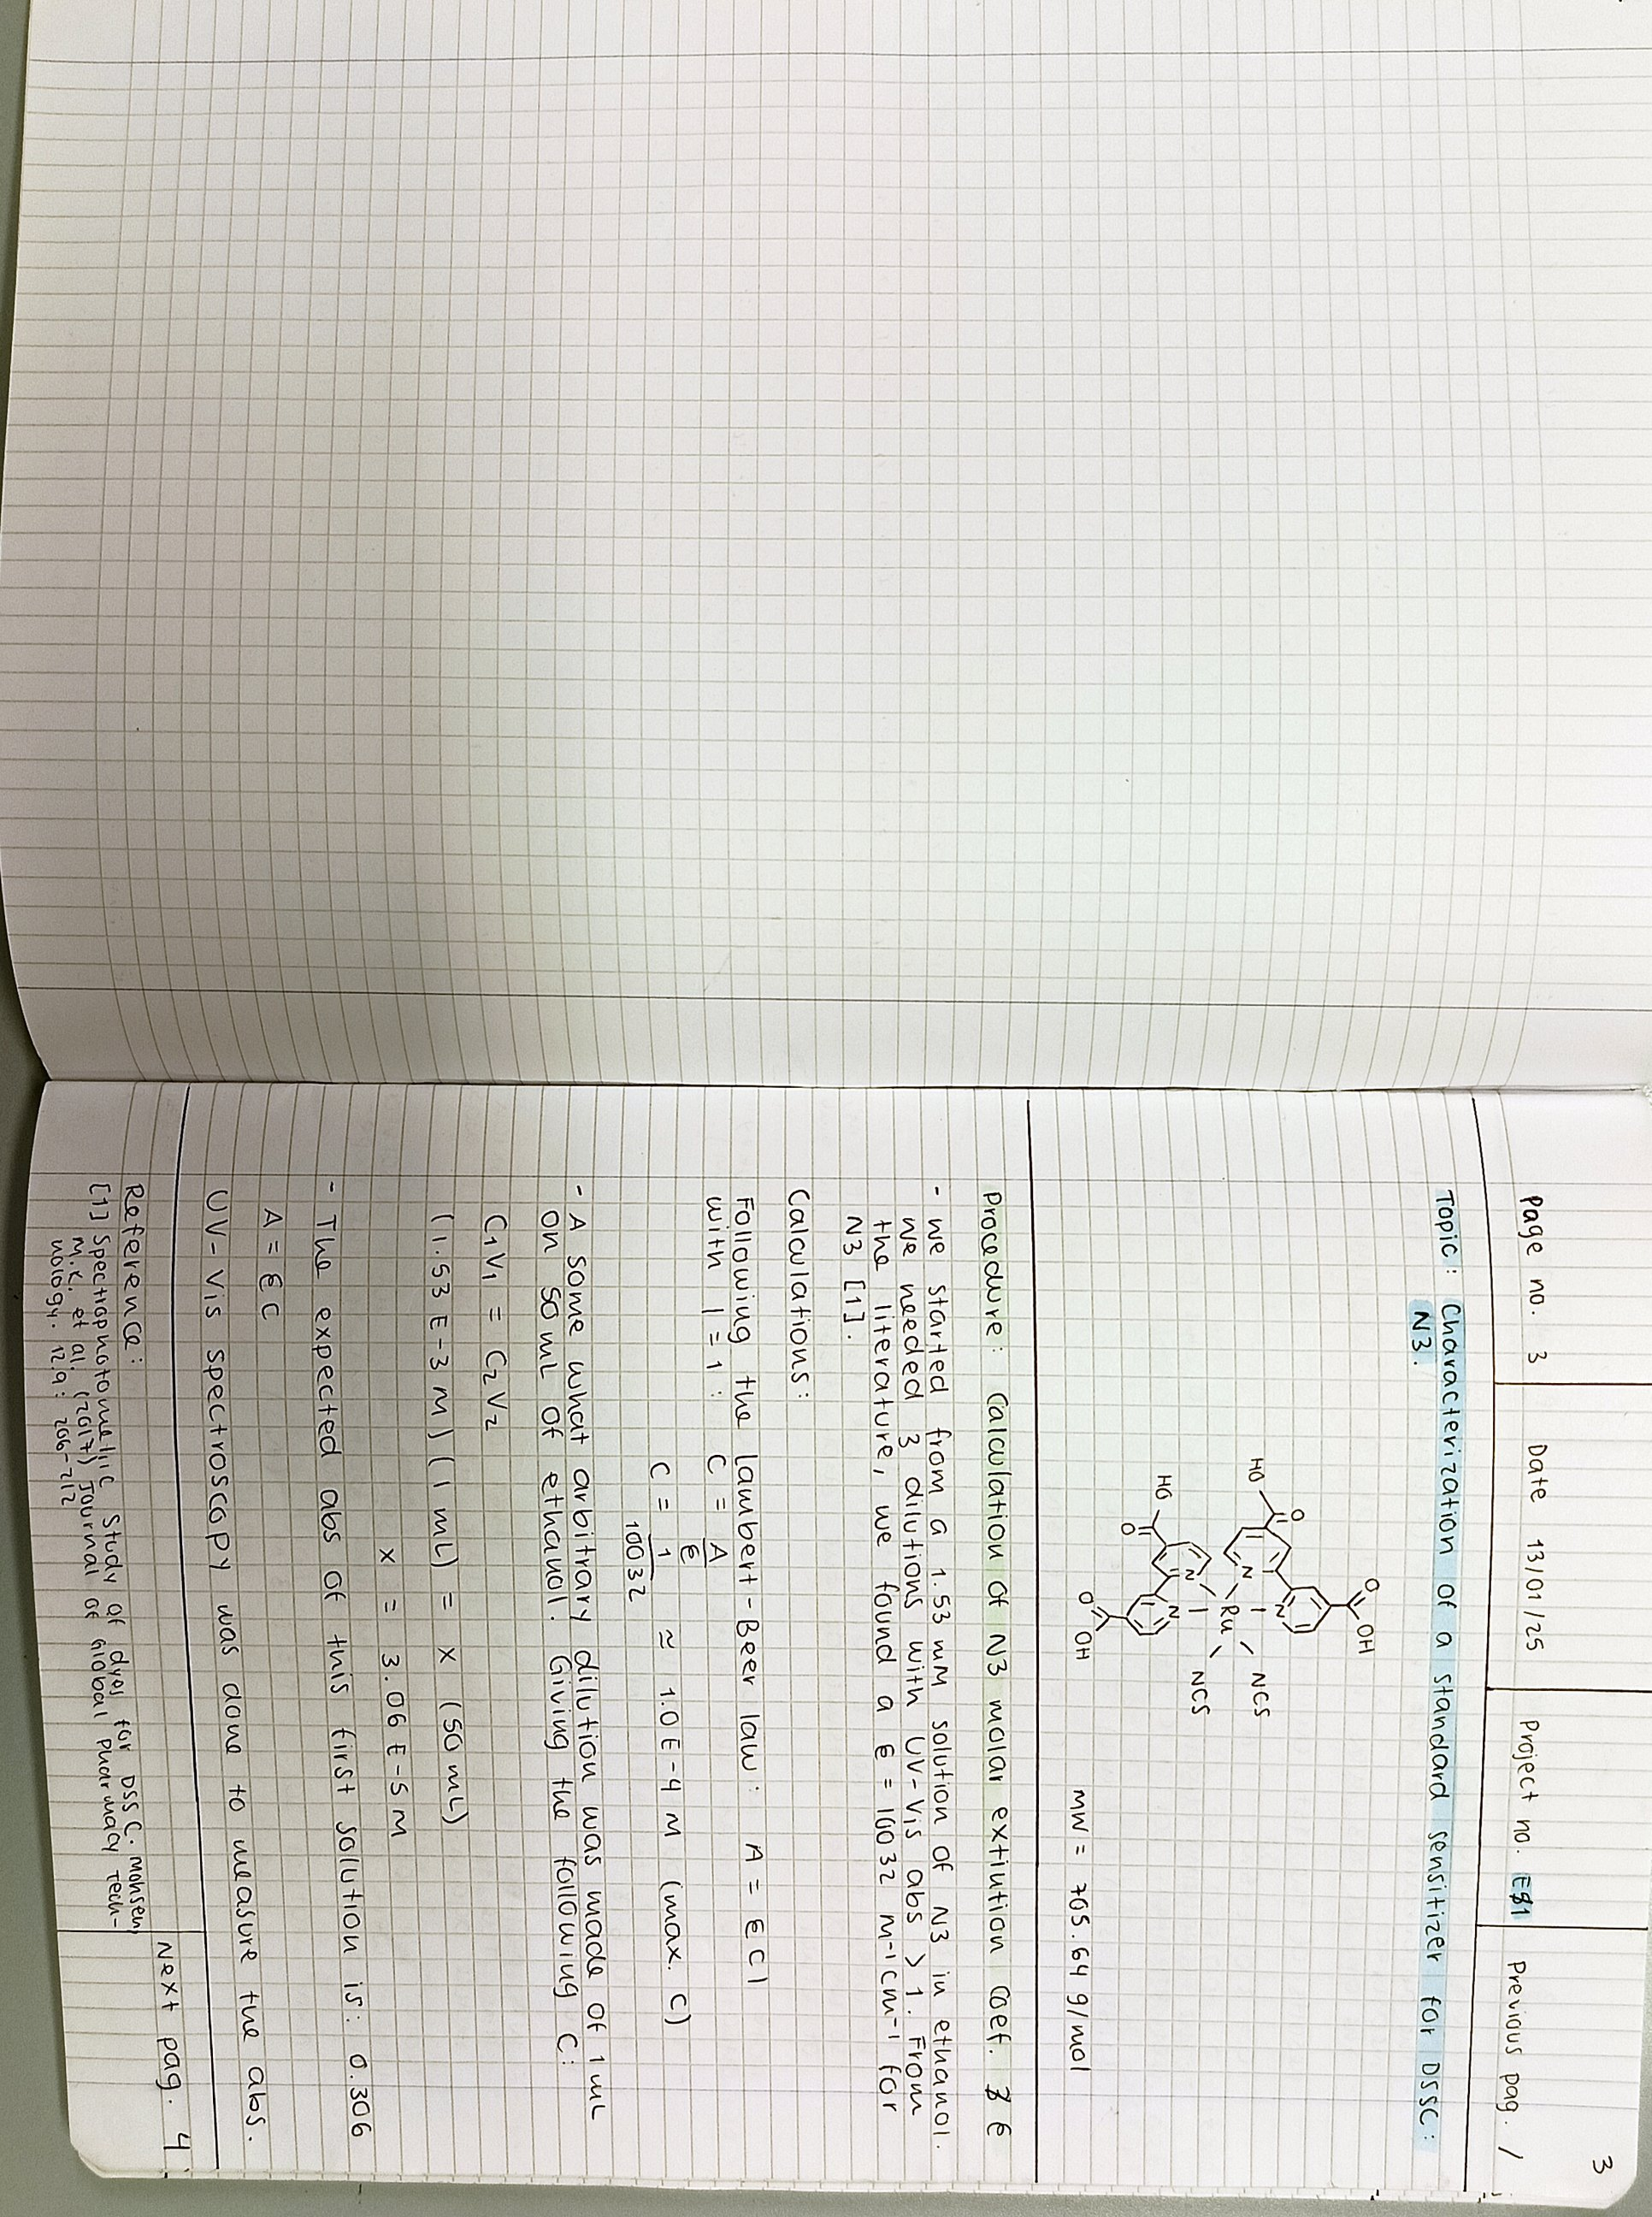
\includegraphics[width=0.6\linewidth, angle=90]{../images/compressed/IMG20250123172849.jpg}
\end{figure}
\begin{figure}[H]
	\centering
	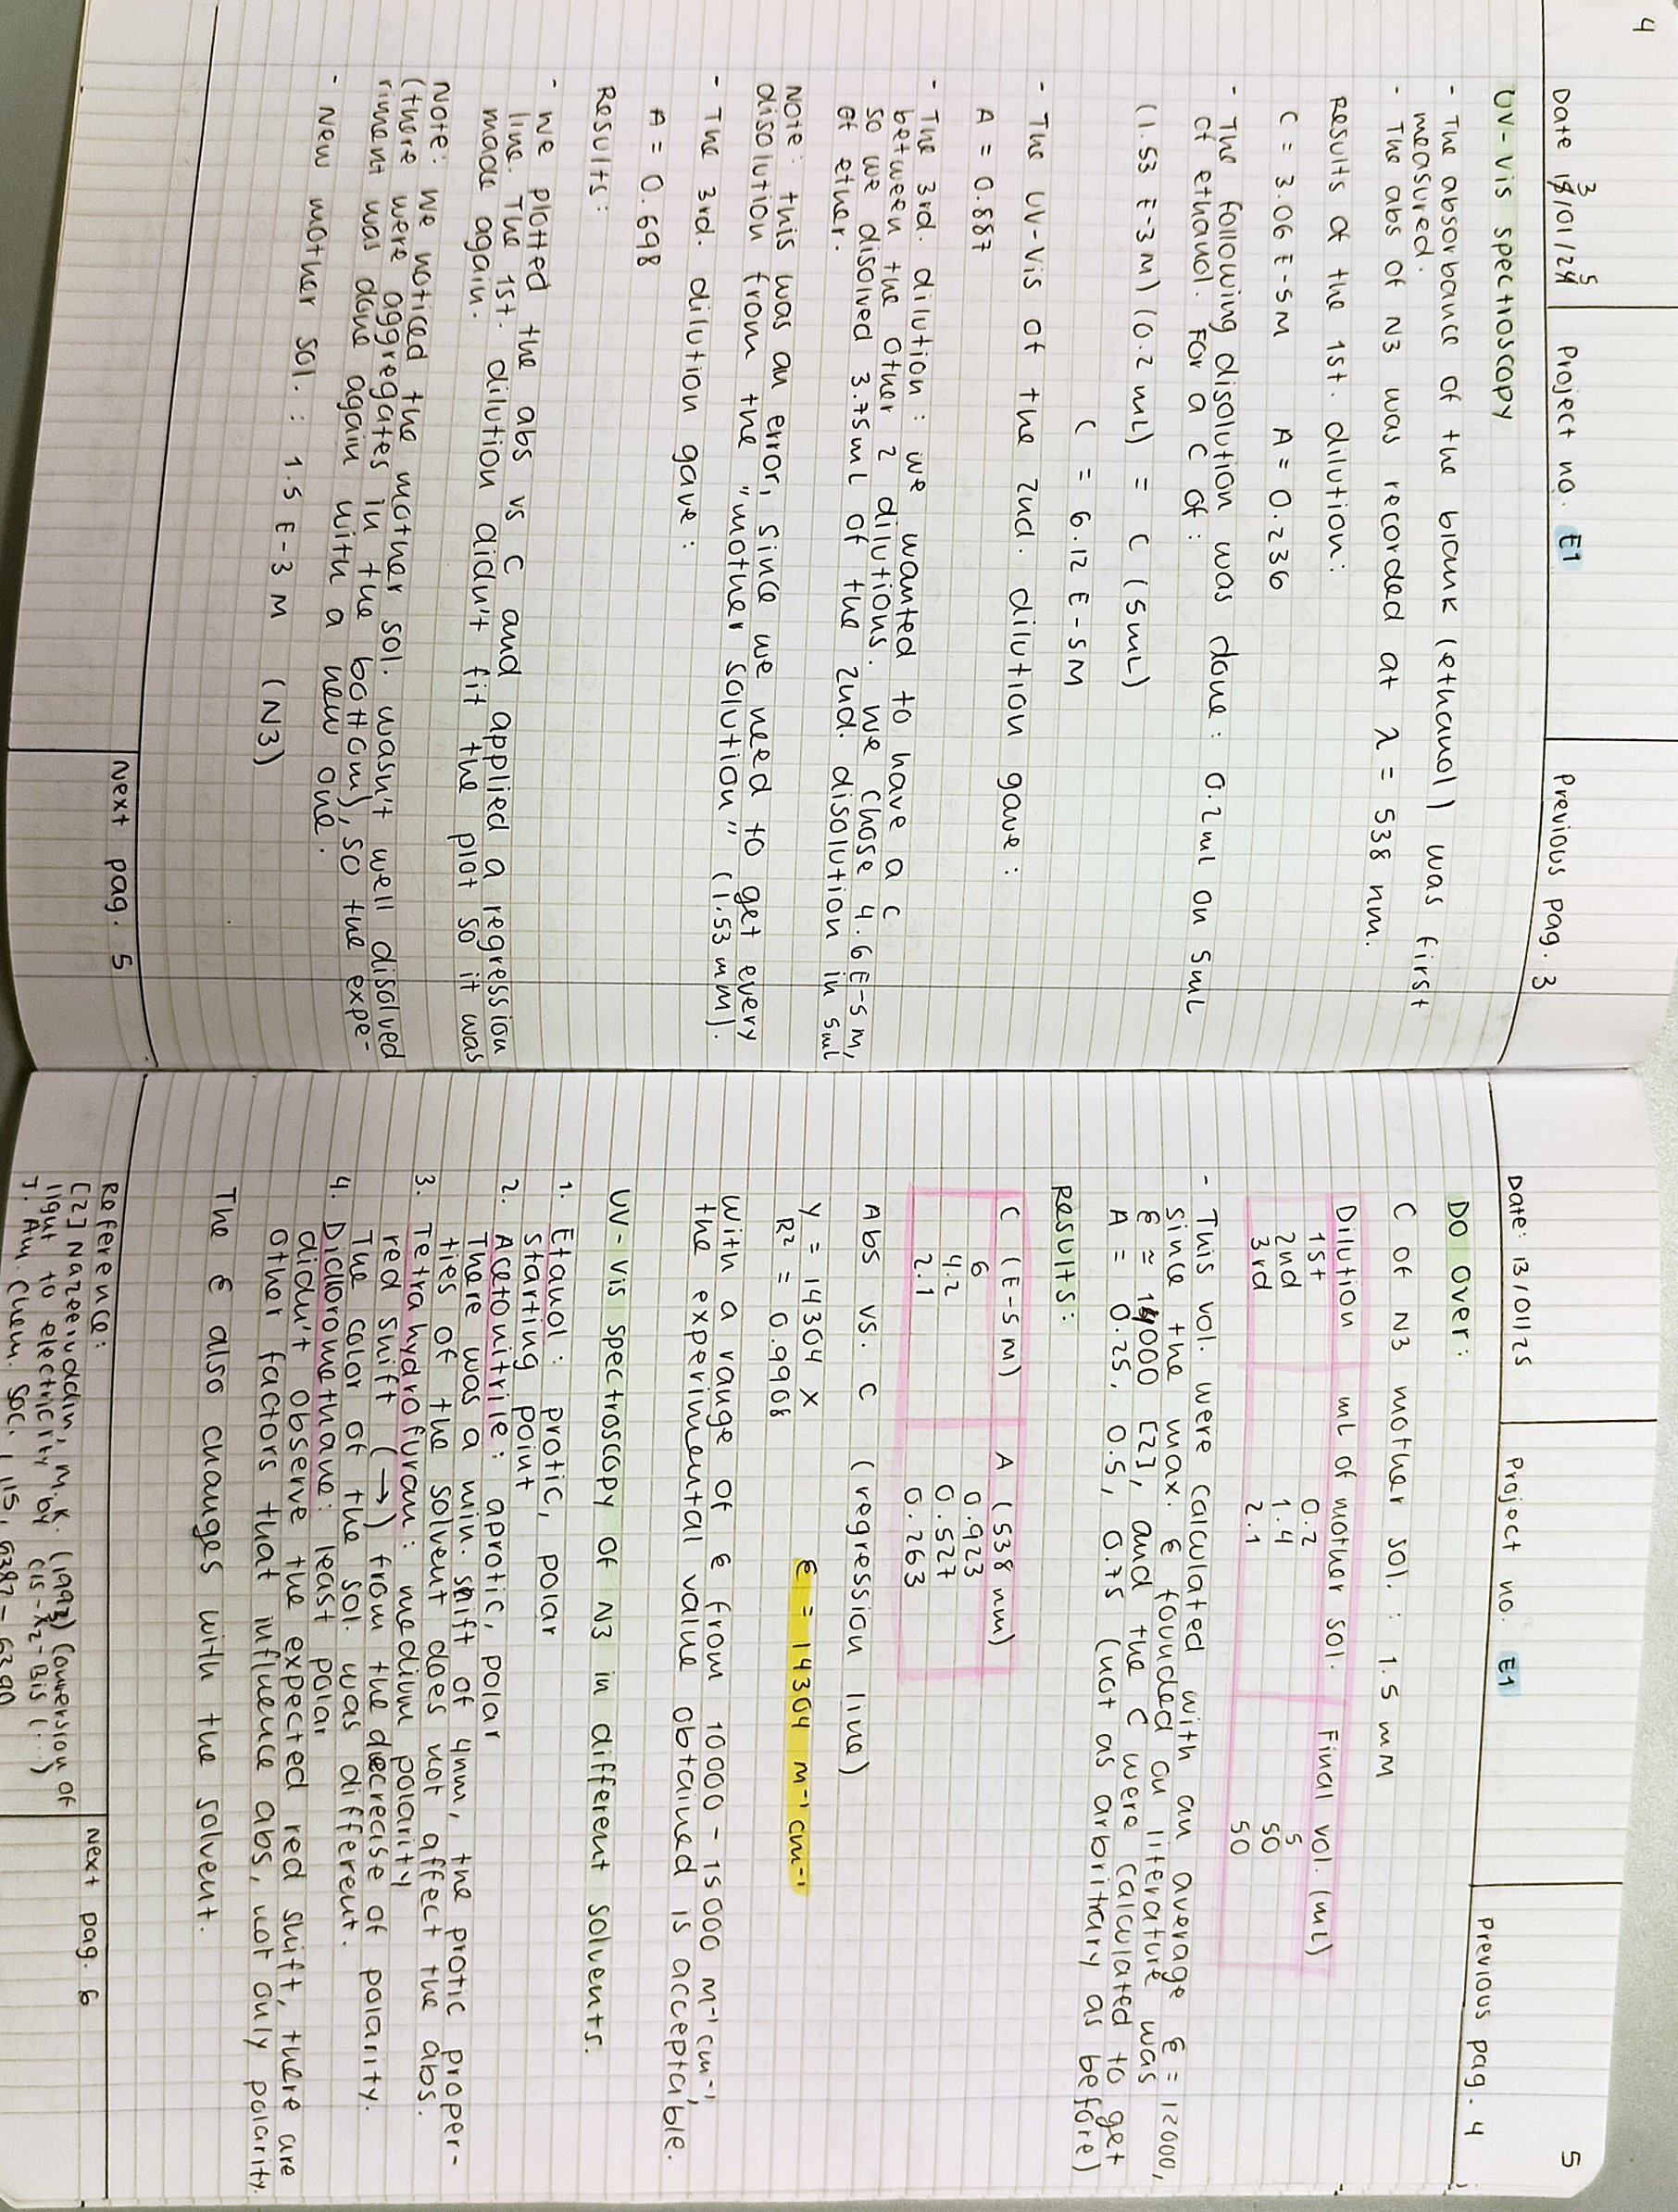
\includegraphics[width=0.6\linewidth, angle=90]{../images/compressed/IMG20250123172905.jpg}
\end{figure}


\subsection{E4}
\begin{figure}[H]
	\centering
	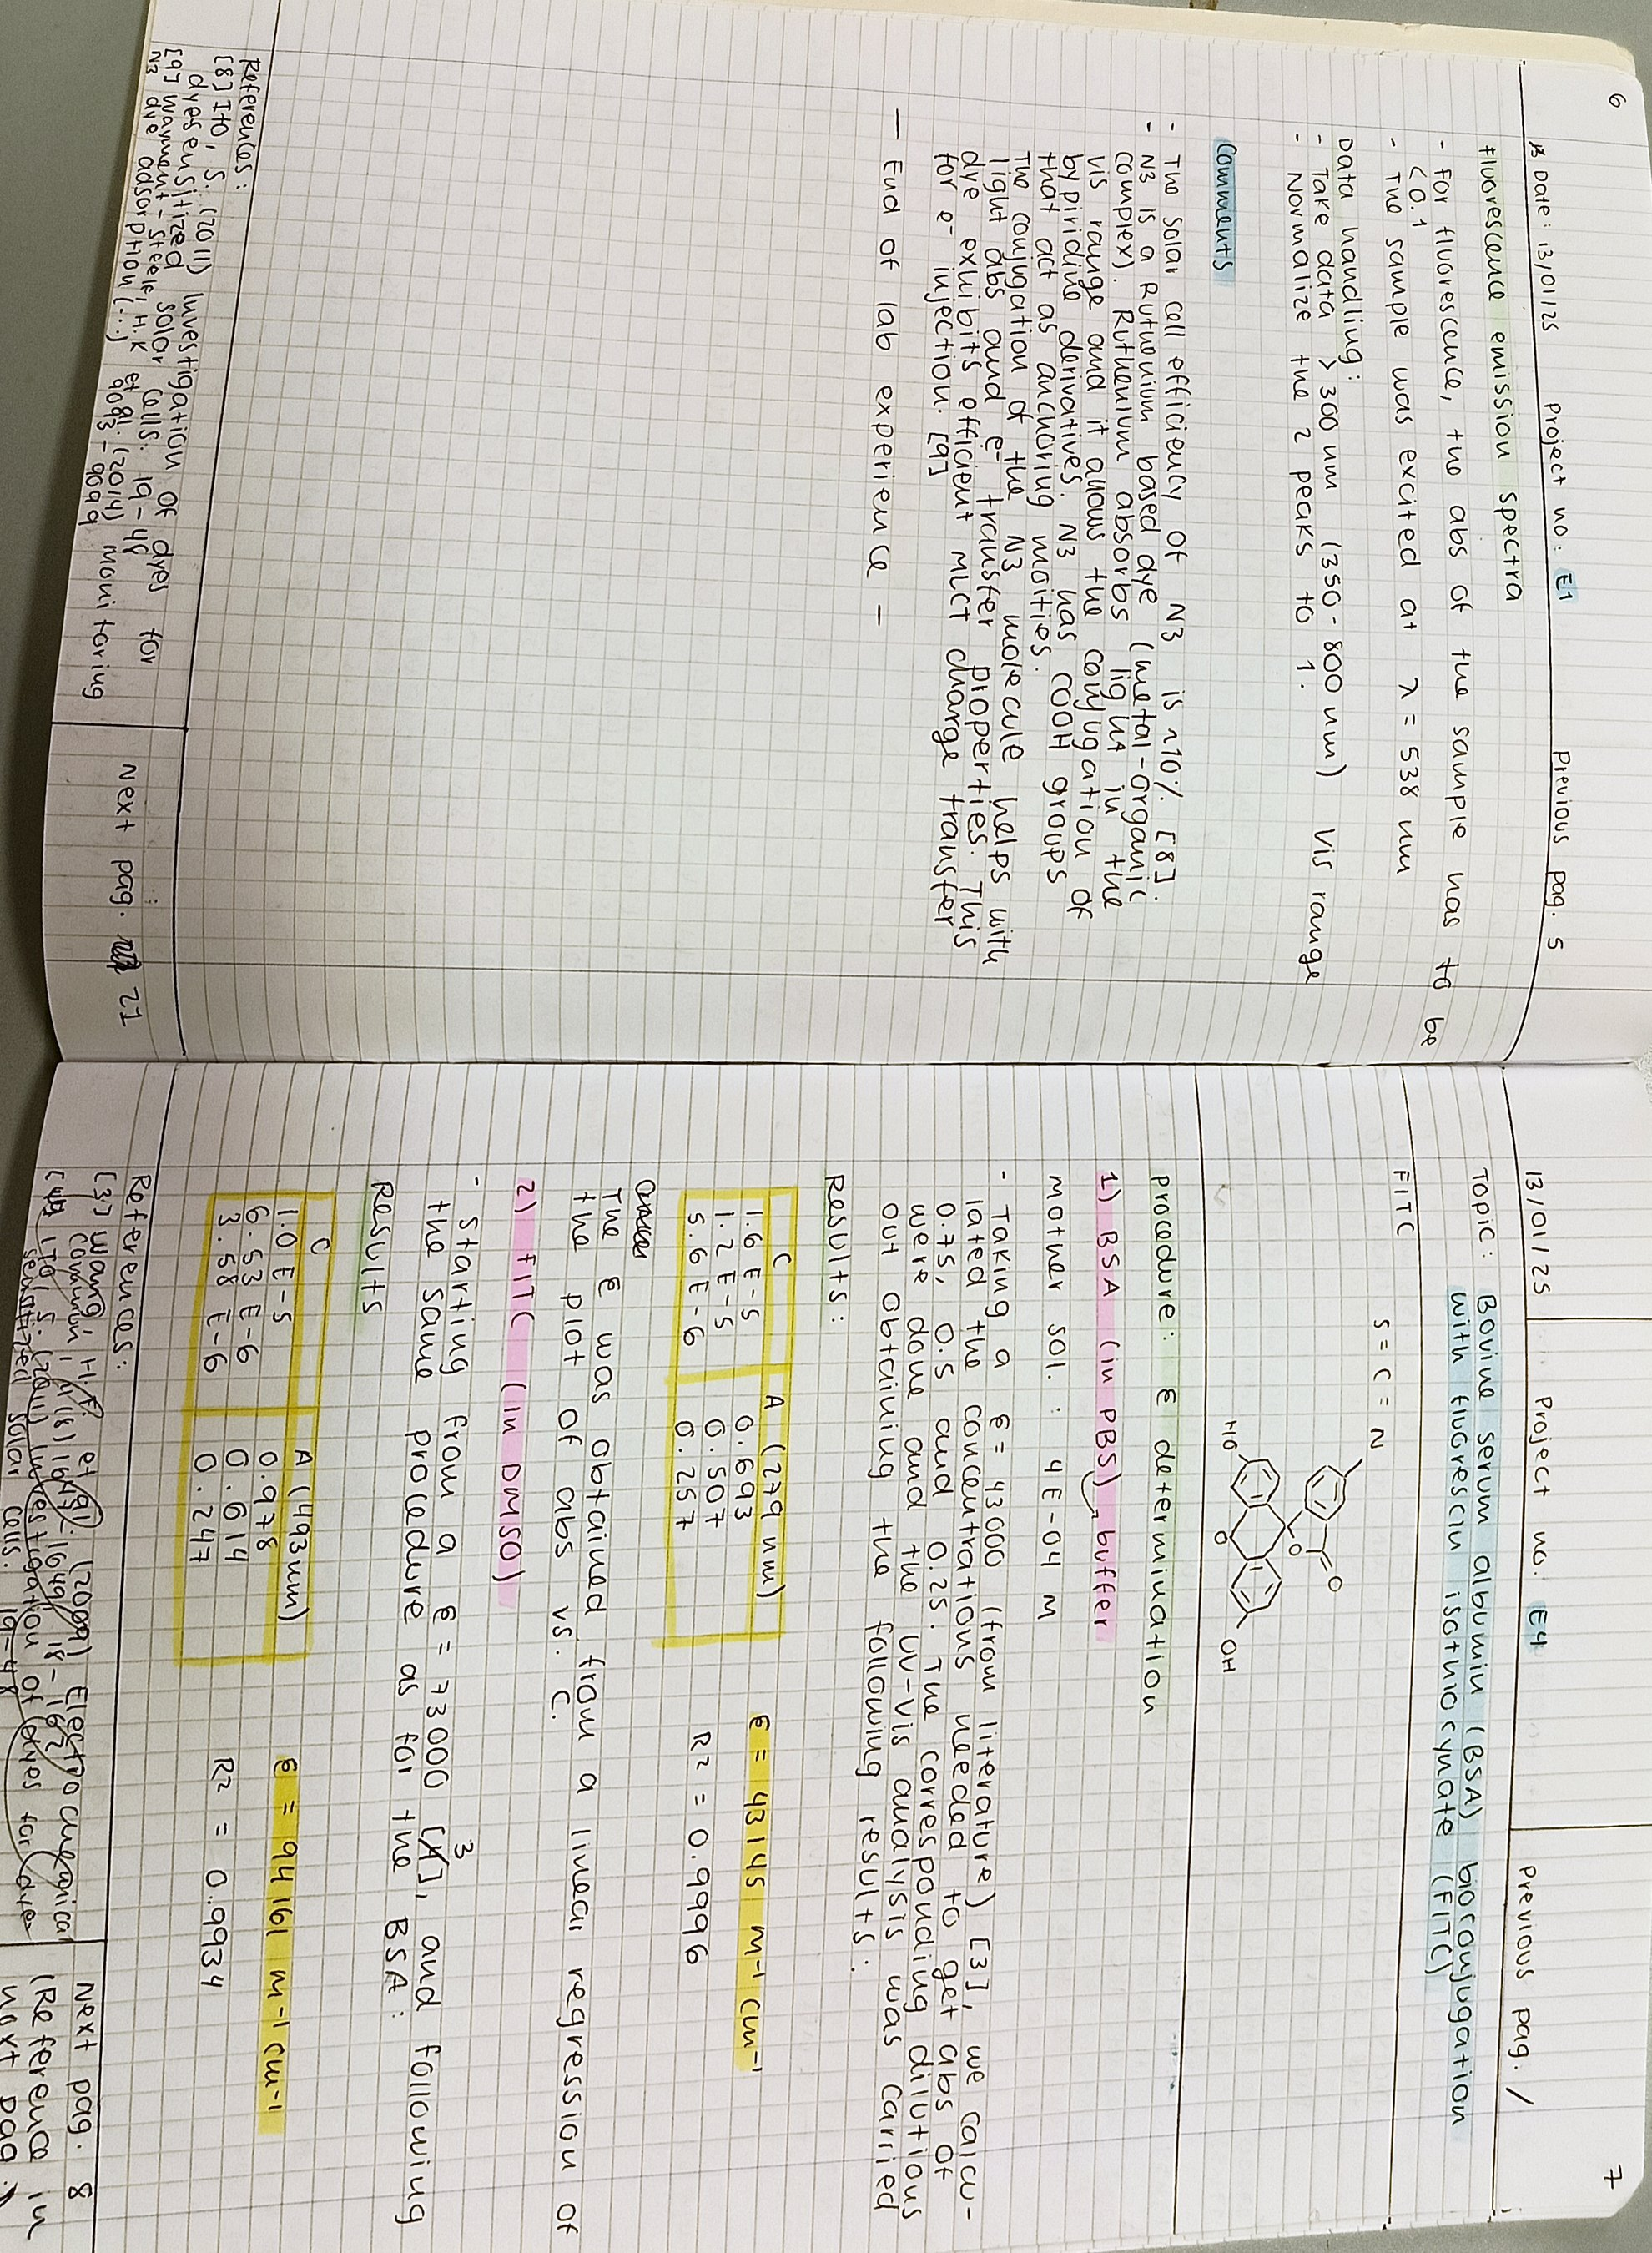
\includegraphics[width=0.6\linewidth, angle=90]{../images/compressed/IMG20250123172914.jpg}
\end{figure}
\begin{figure}[H]
	\centering
	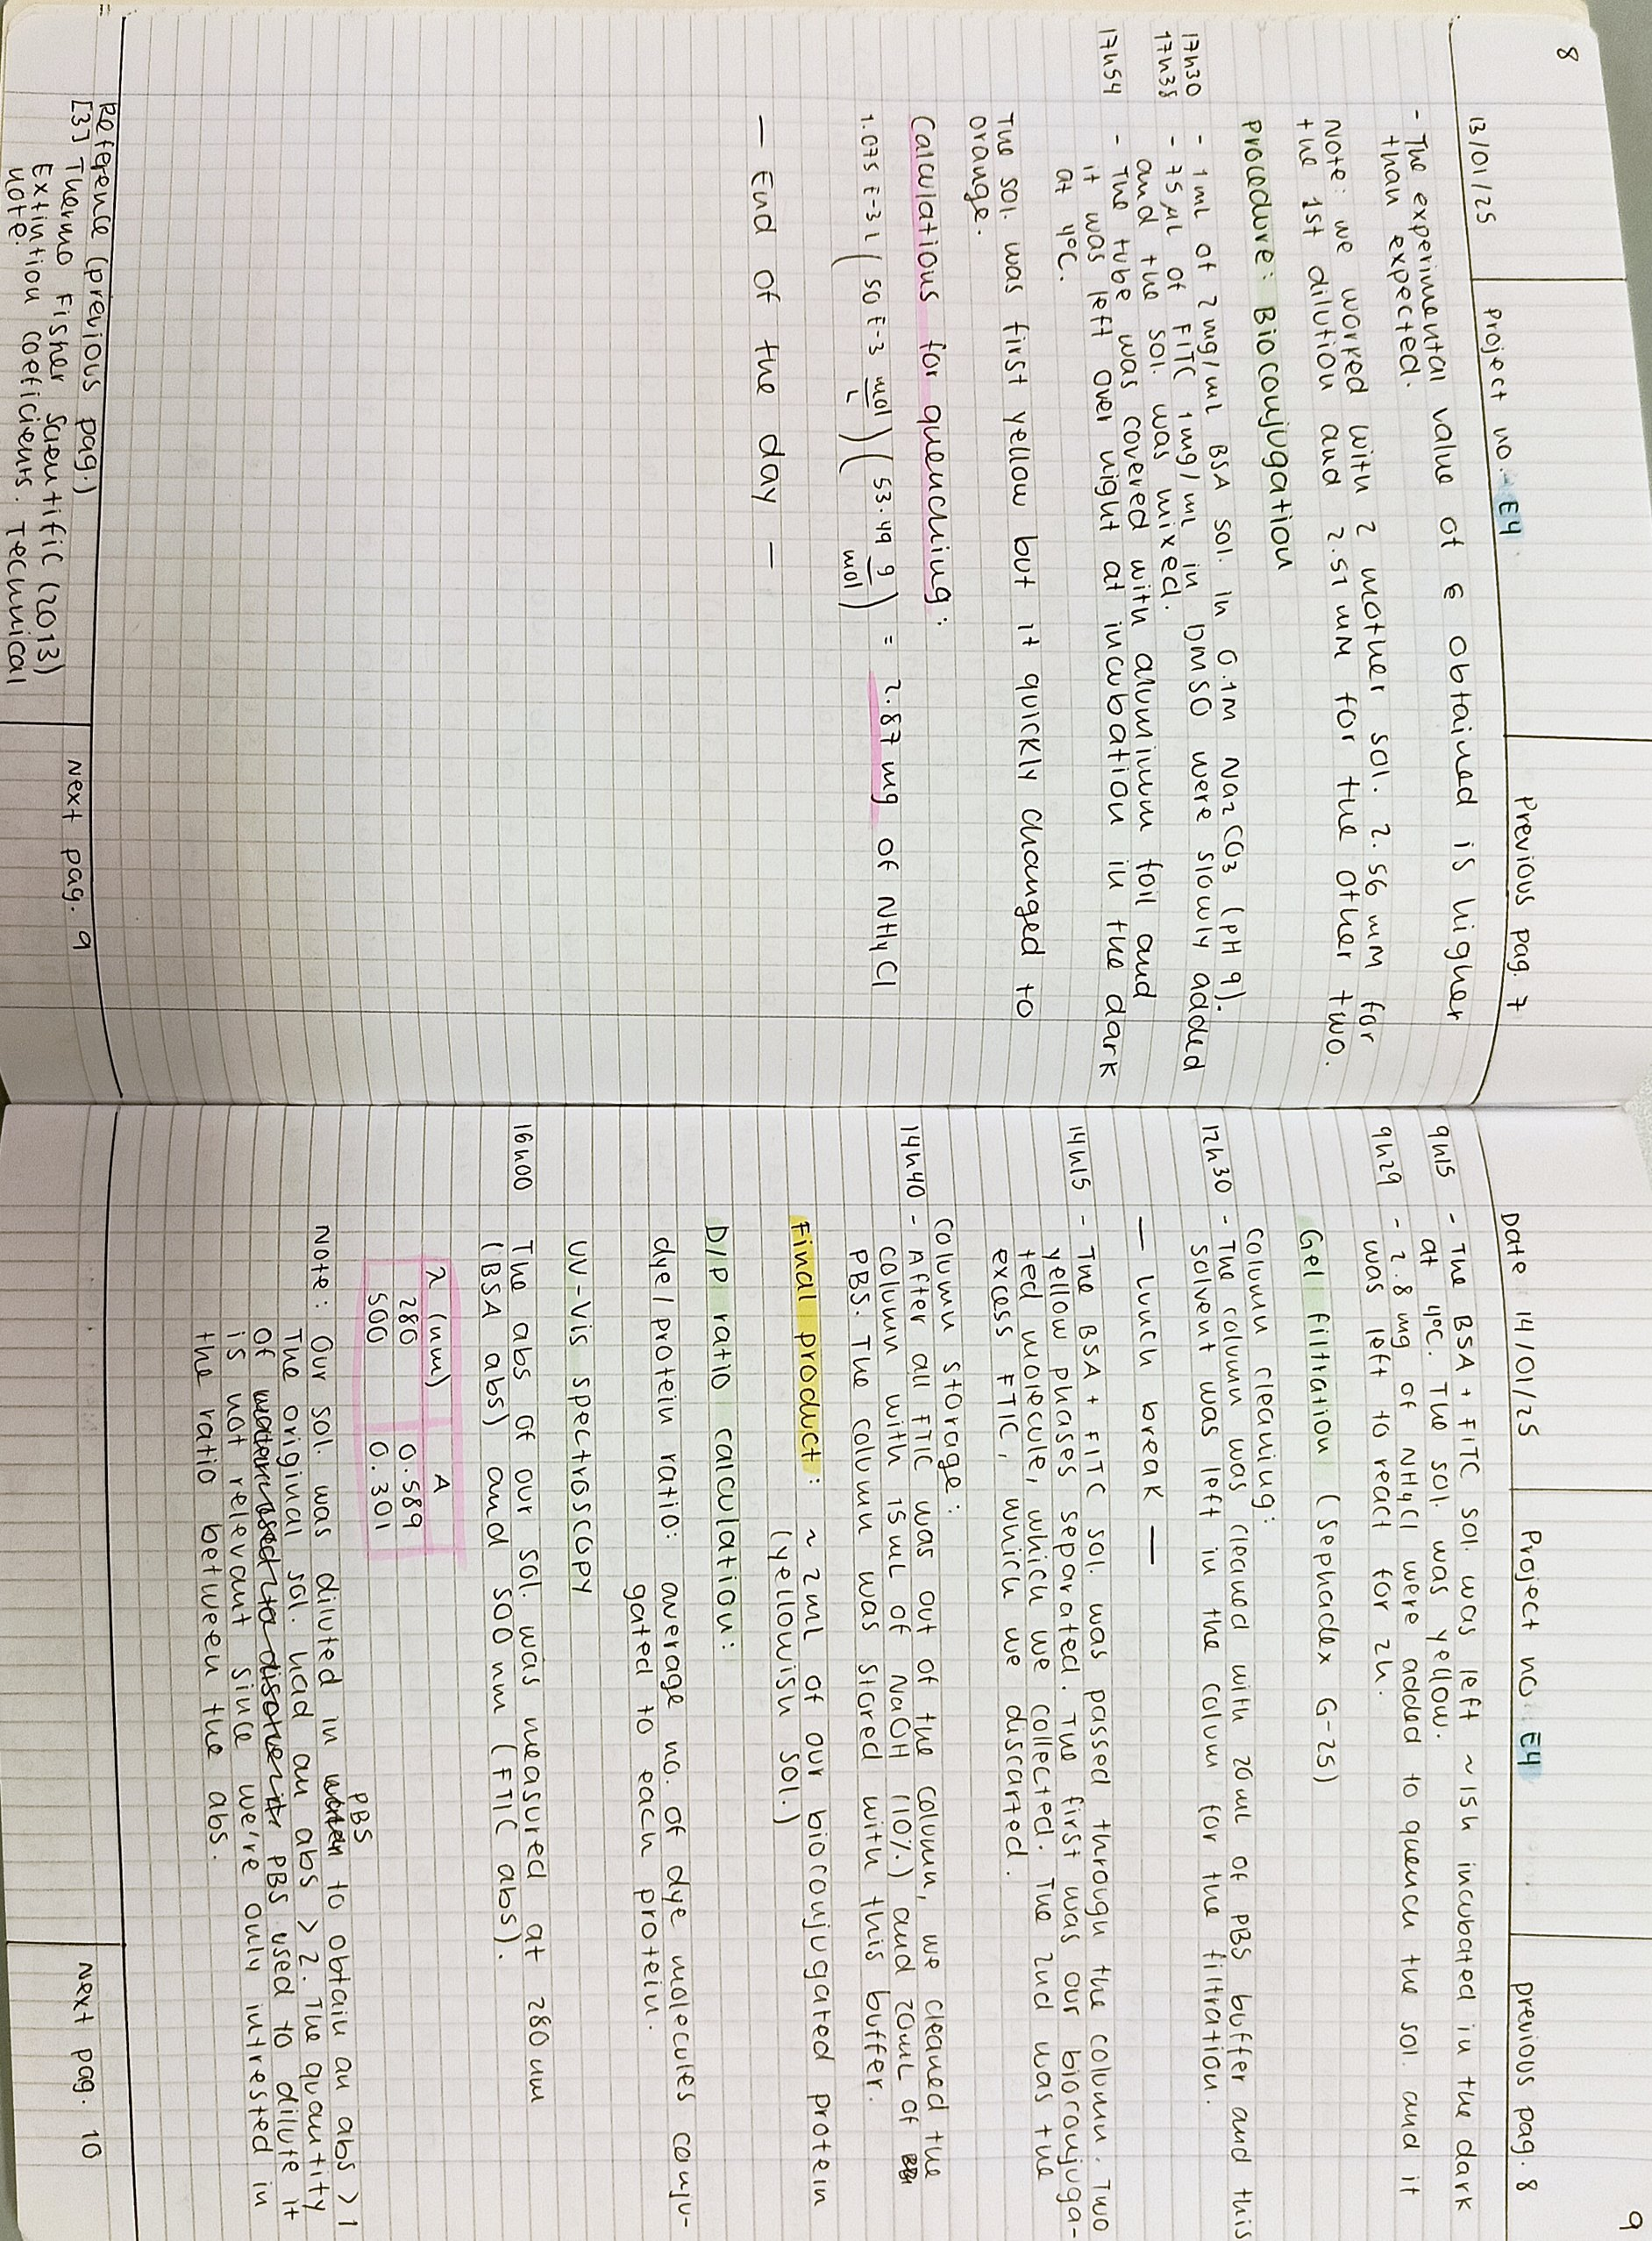
\includegraphics[width=0.6\linewidth, angle=90]{../images/compressed/IMG20250123172932.jpg}
\end{figure}


\subsection{E3}
\begin{figure}[H]
	\centering
	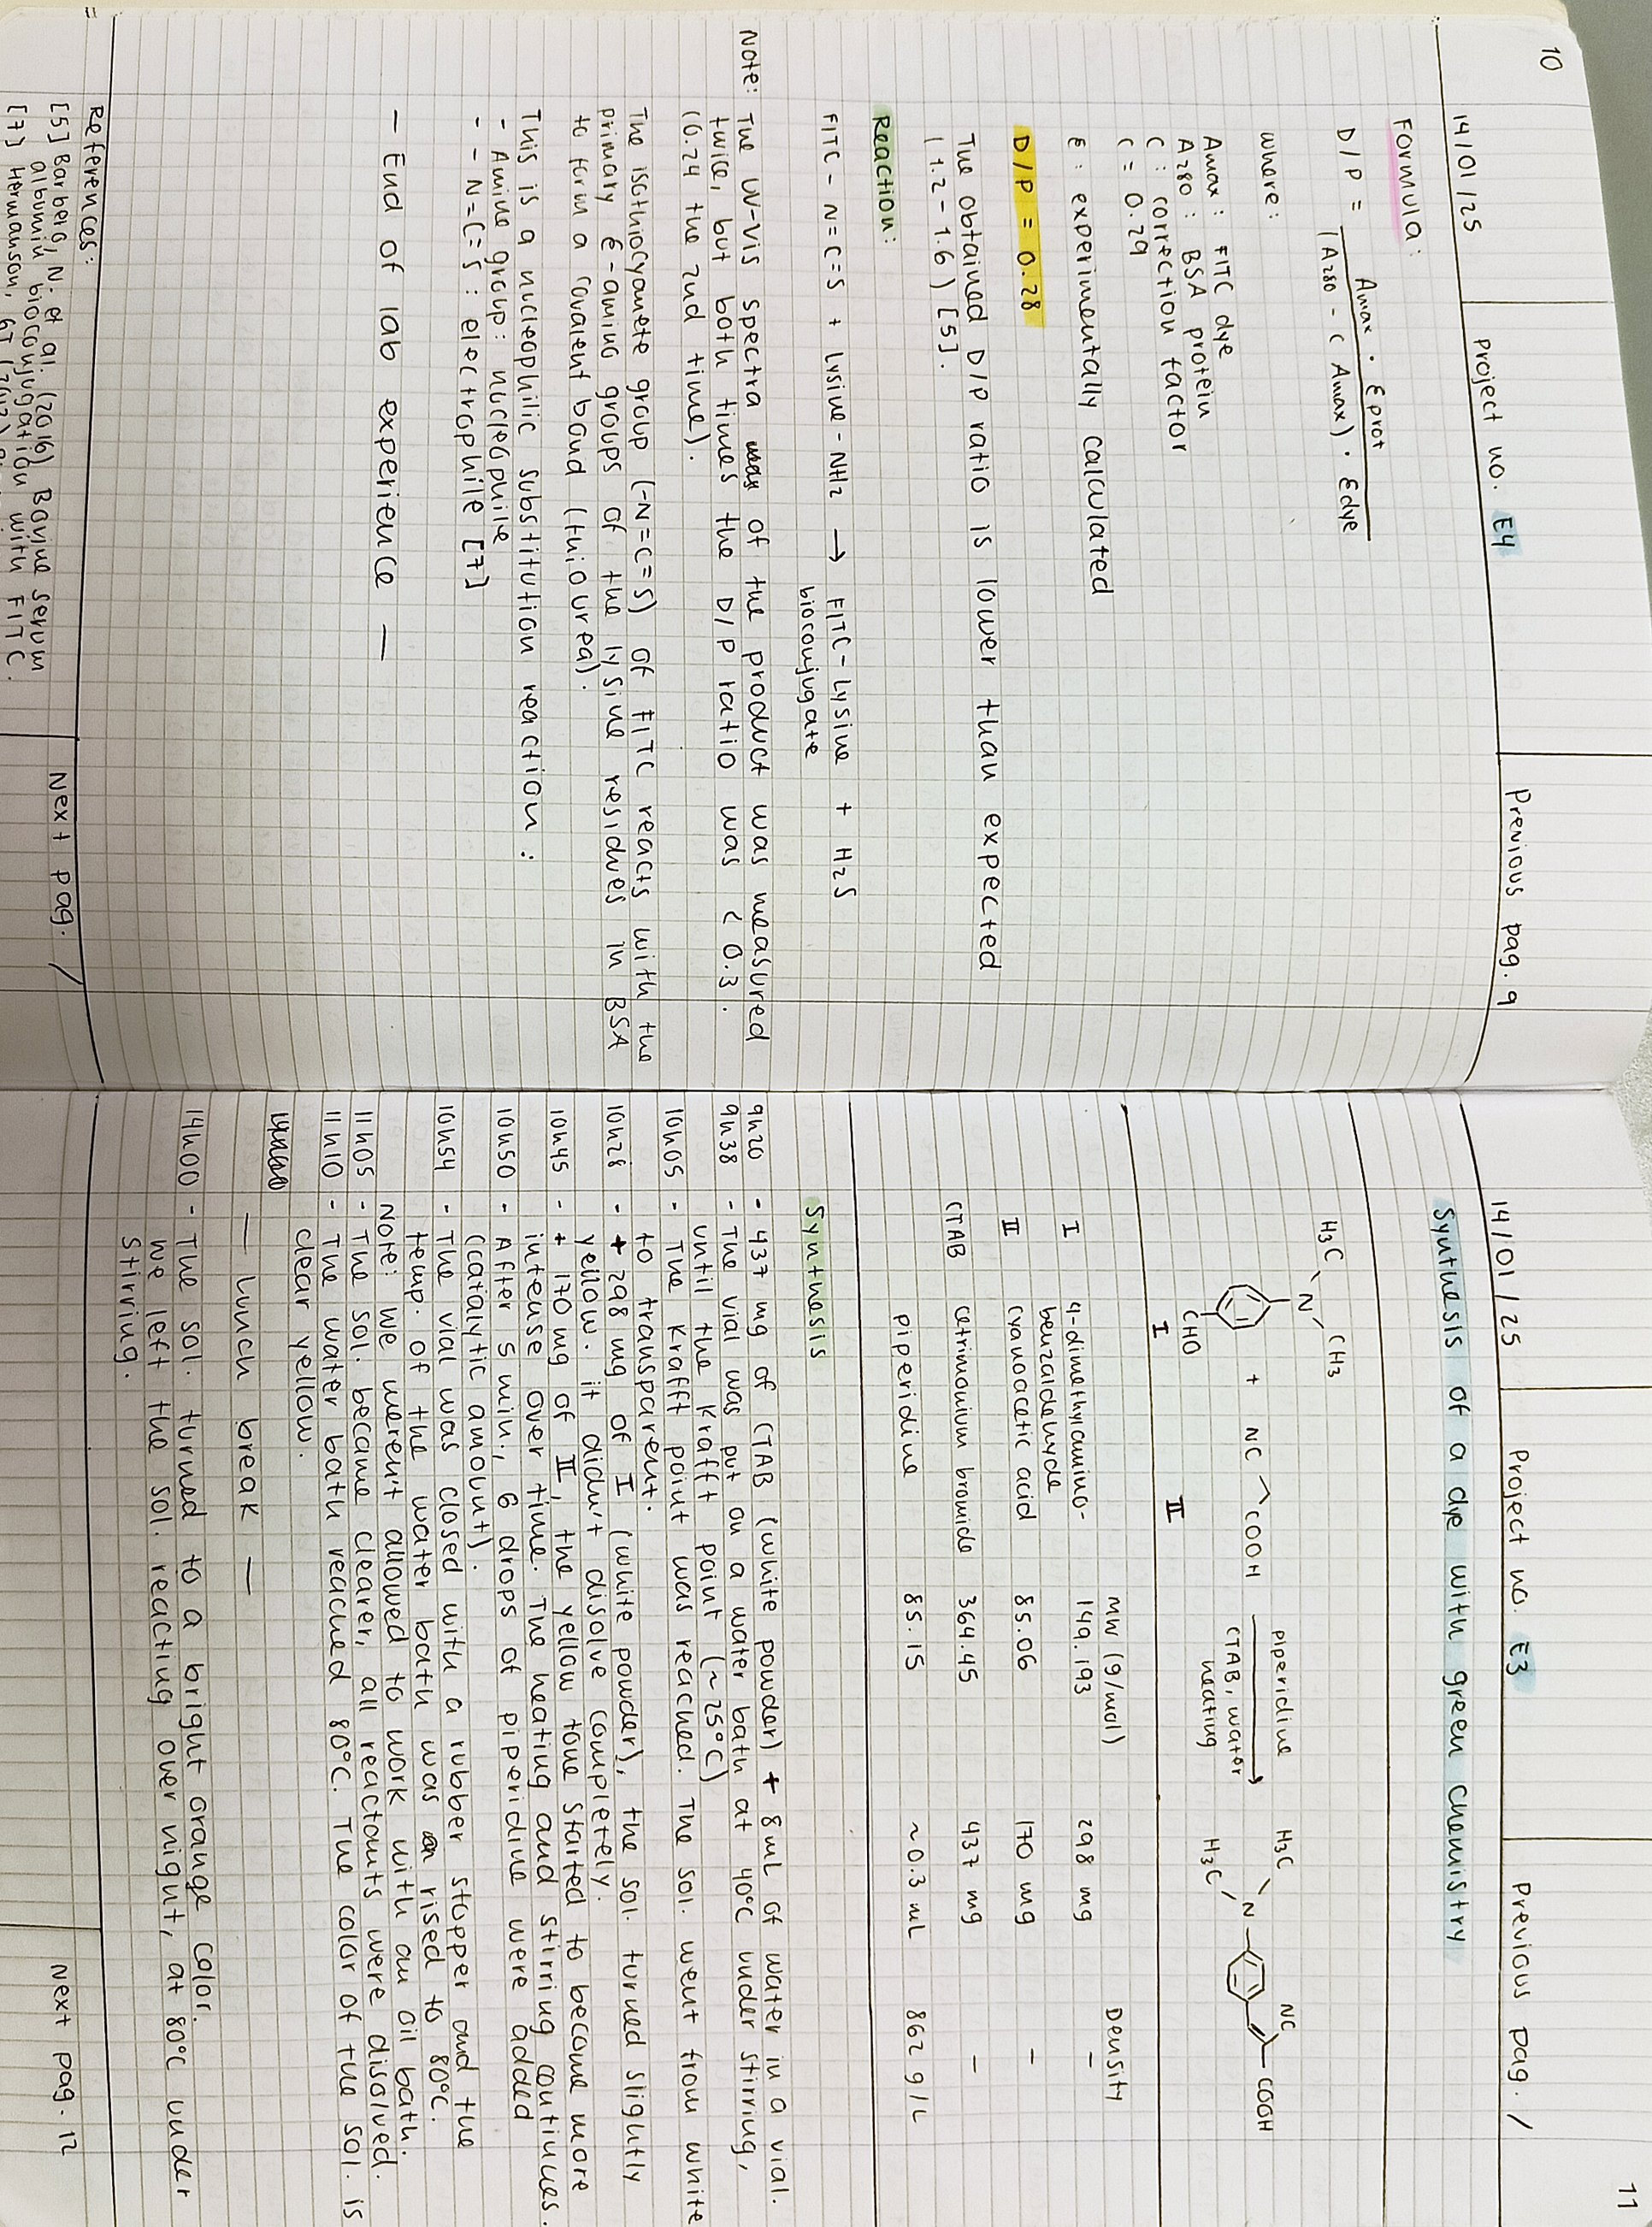
\includegraphics[width=0.6\linewidth, angle=90]{../images/compressed/IMG20250123172939.jpg}
\end{figure}
\begin{figure}[H]
	\centering
	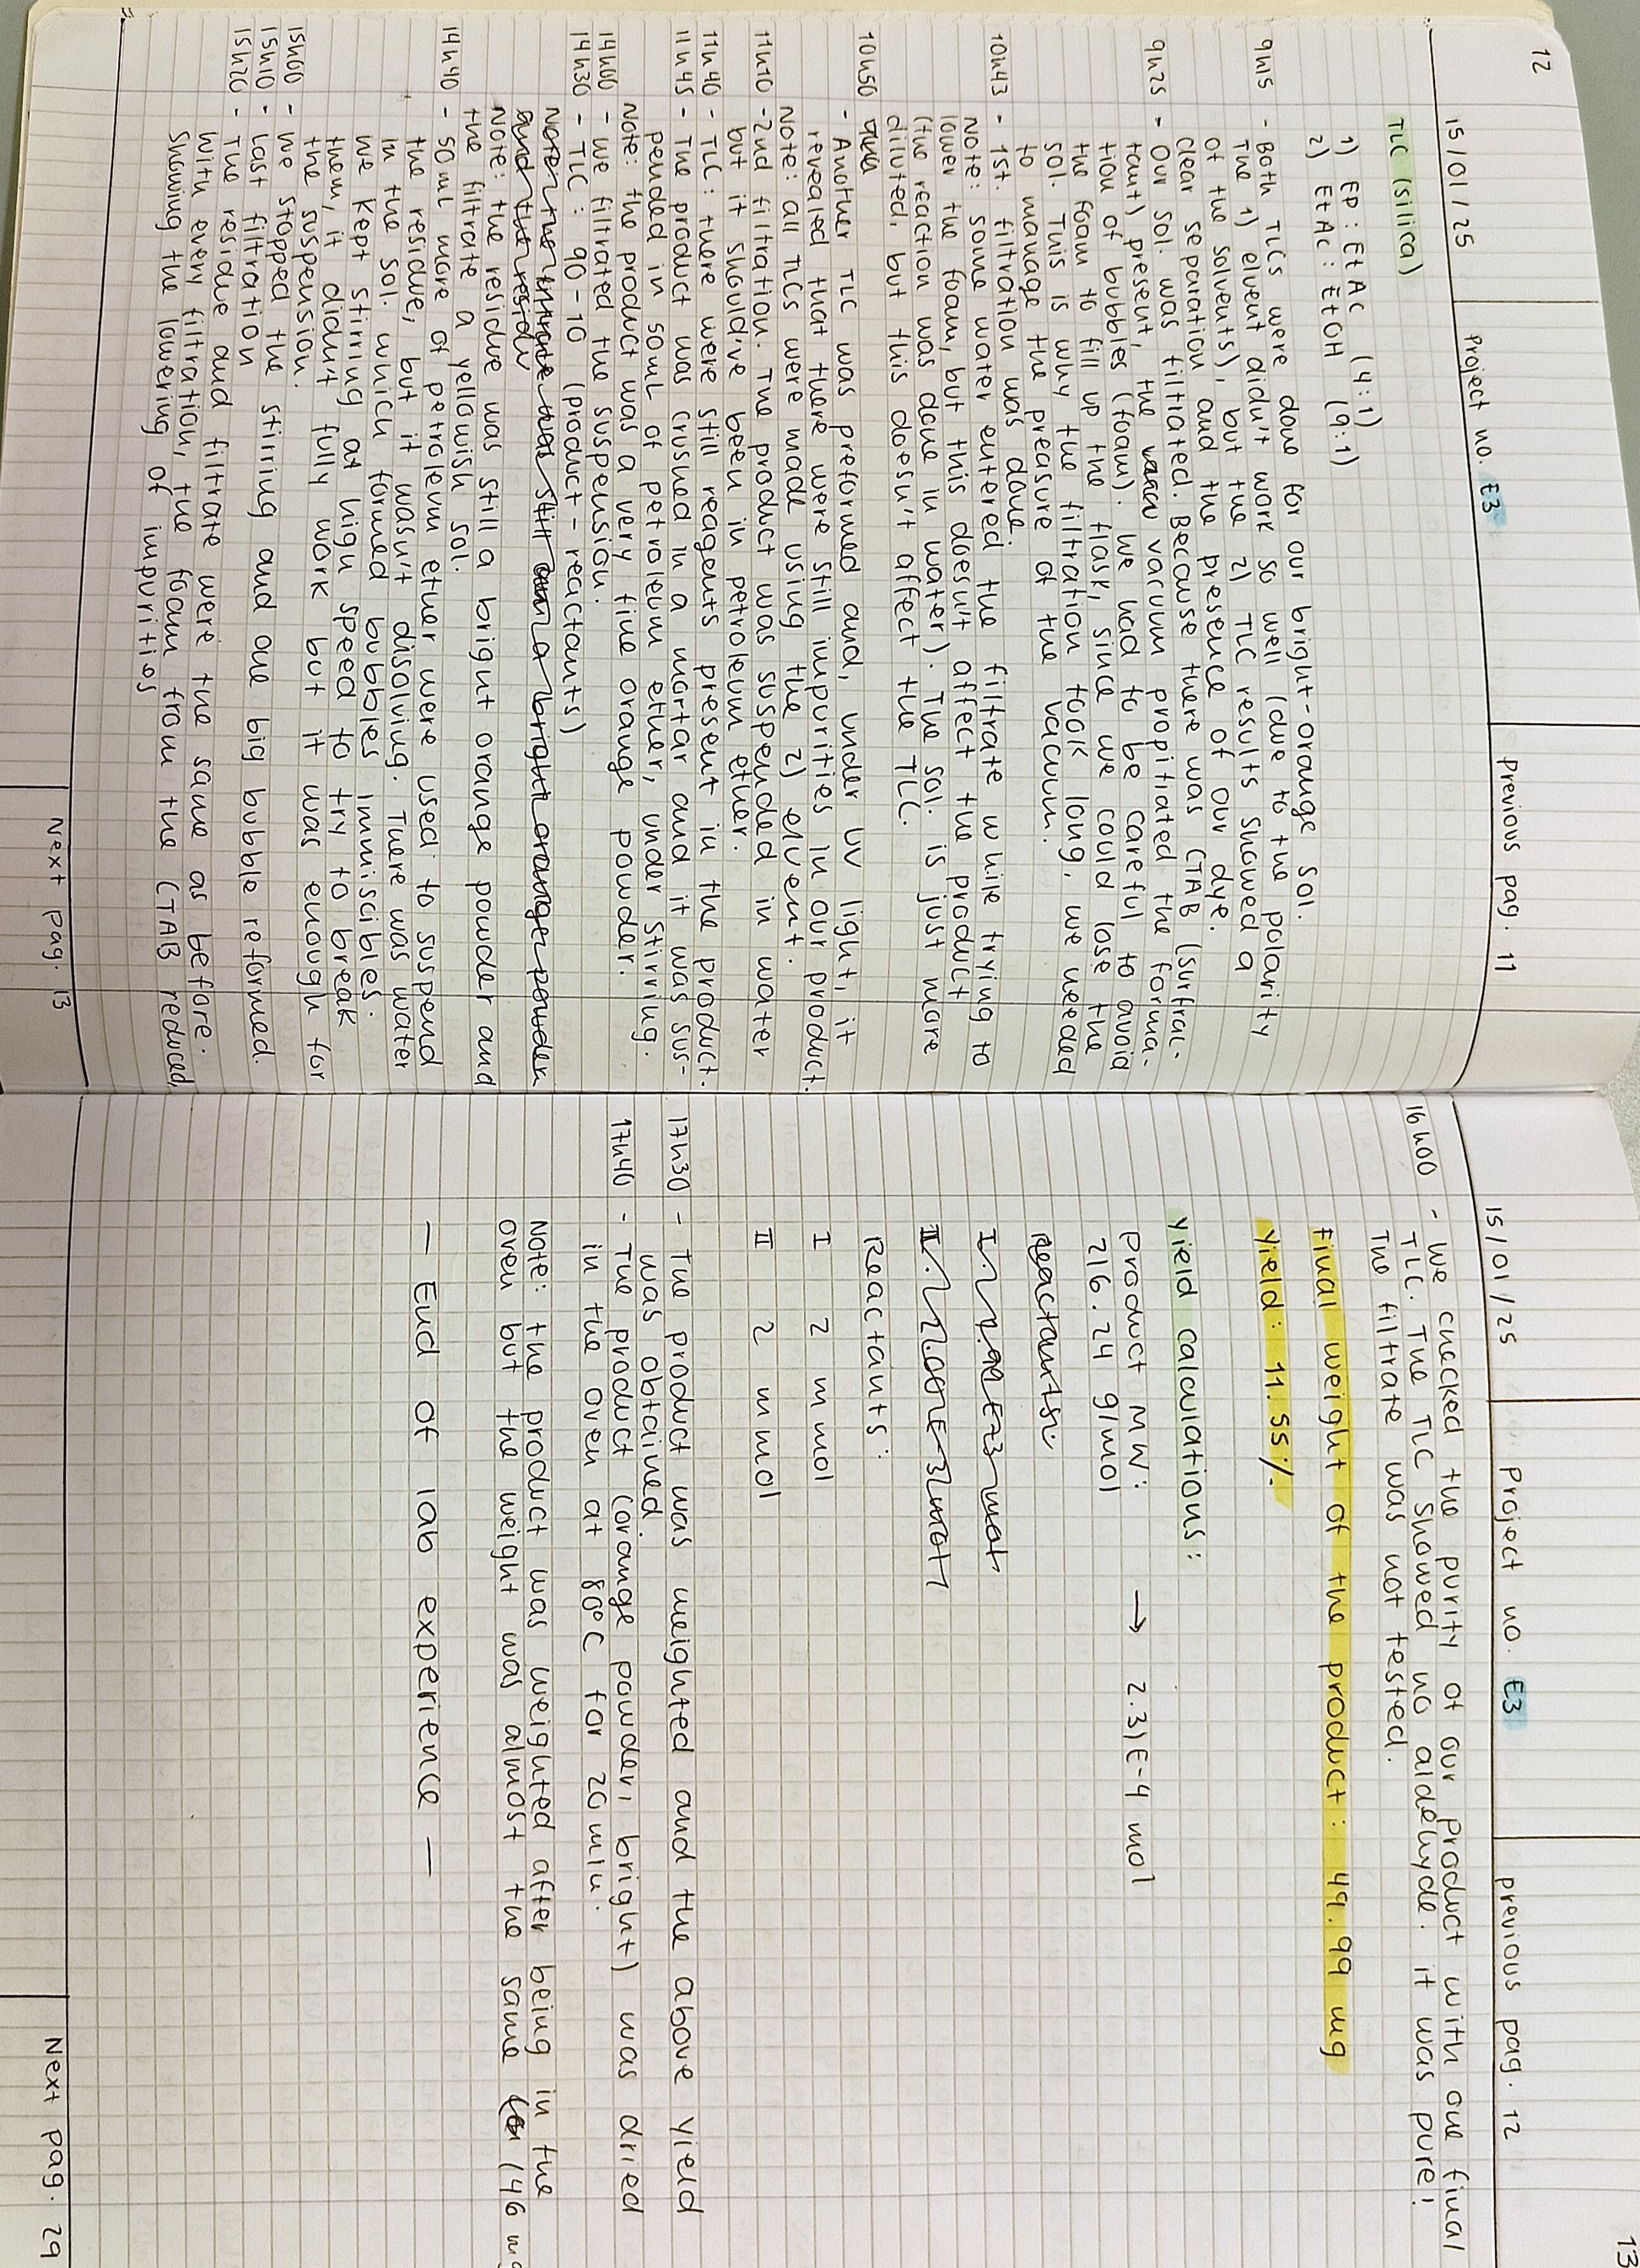
\includegraphics[width=0.6\linewidth, angle=90]{../images/compressed/IMG20250123172945.jpg}
\end{figure}


\subsection{E2}
\begin{figure}[H]
	\centering
	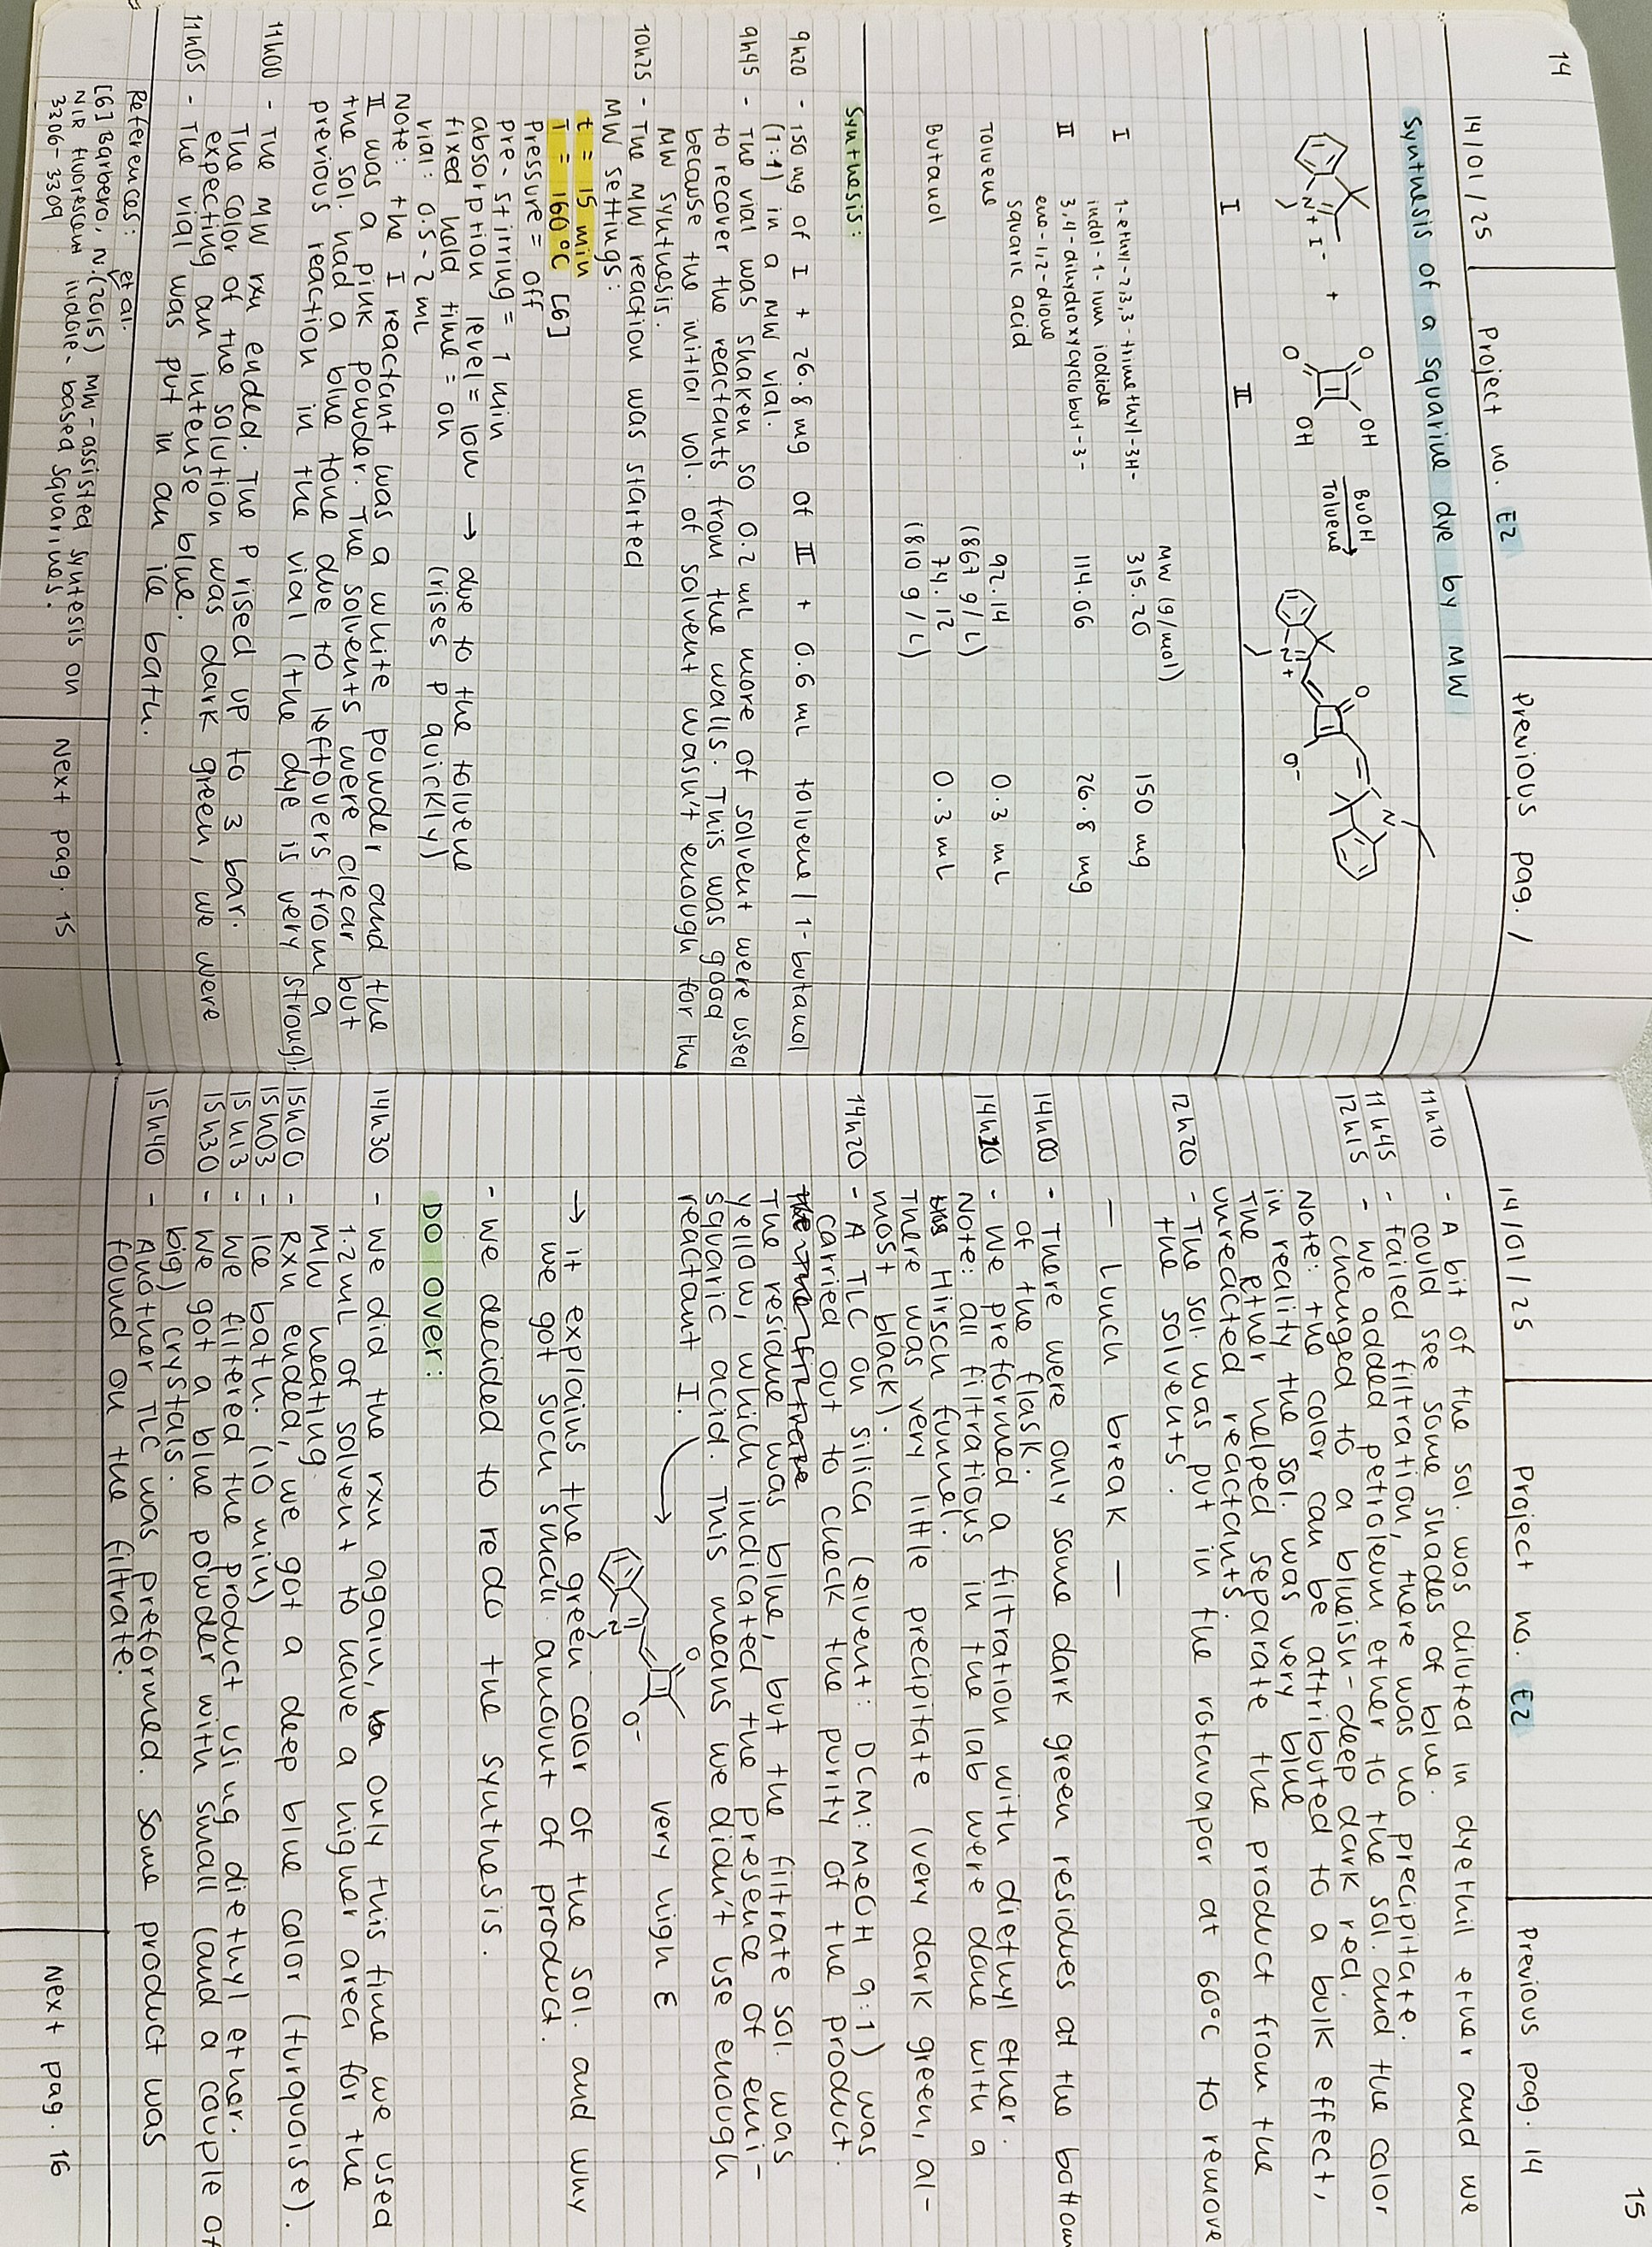
\includegraphics[width=0.6\linewidth, angle=90]{../images/compressed/IMG20250123172951.jpg}
\end{figure}
\begin{figure}[H]
	\centering
	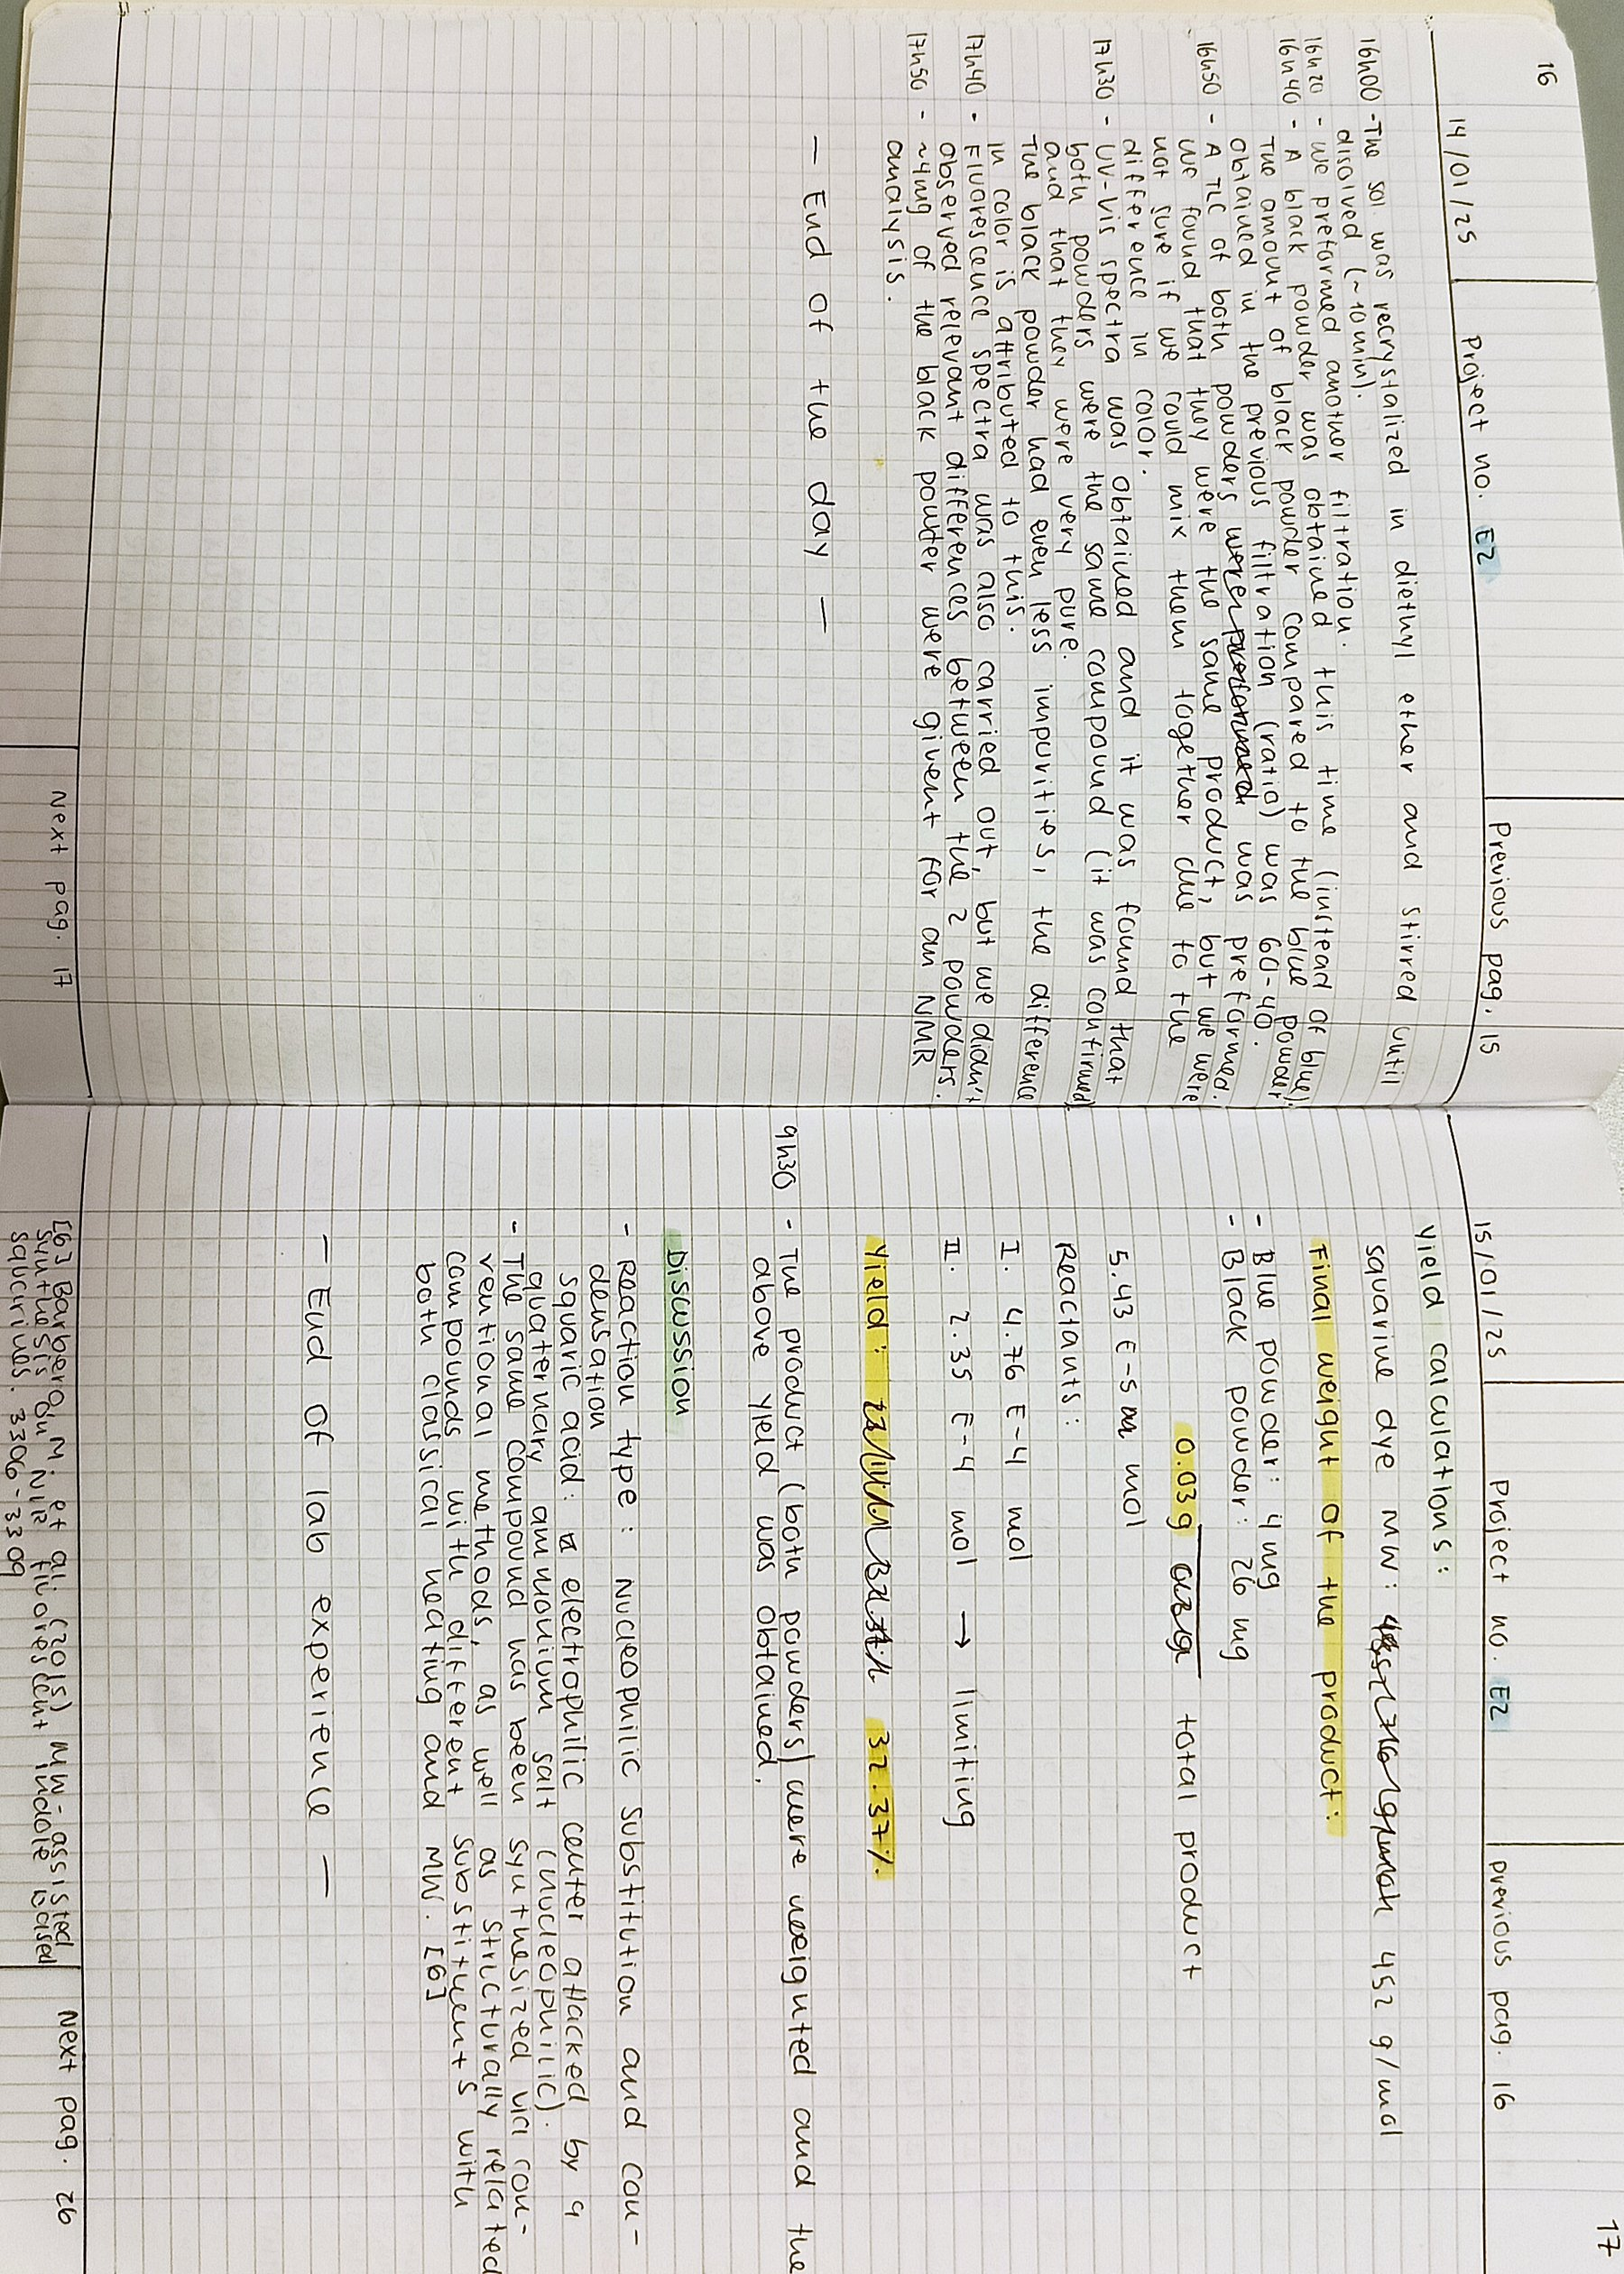
\includegraphics[width=0.6\linewidth, angle=90]{../images/compressed/IMG20250123173003.jpg}
\end{figure}


\subsection{E5}
\begin{figure}[H]
	\centering
	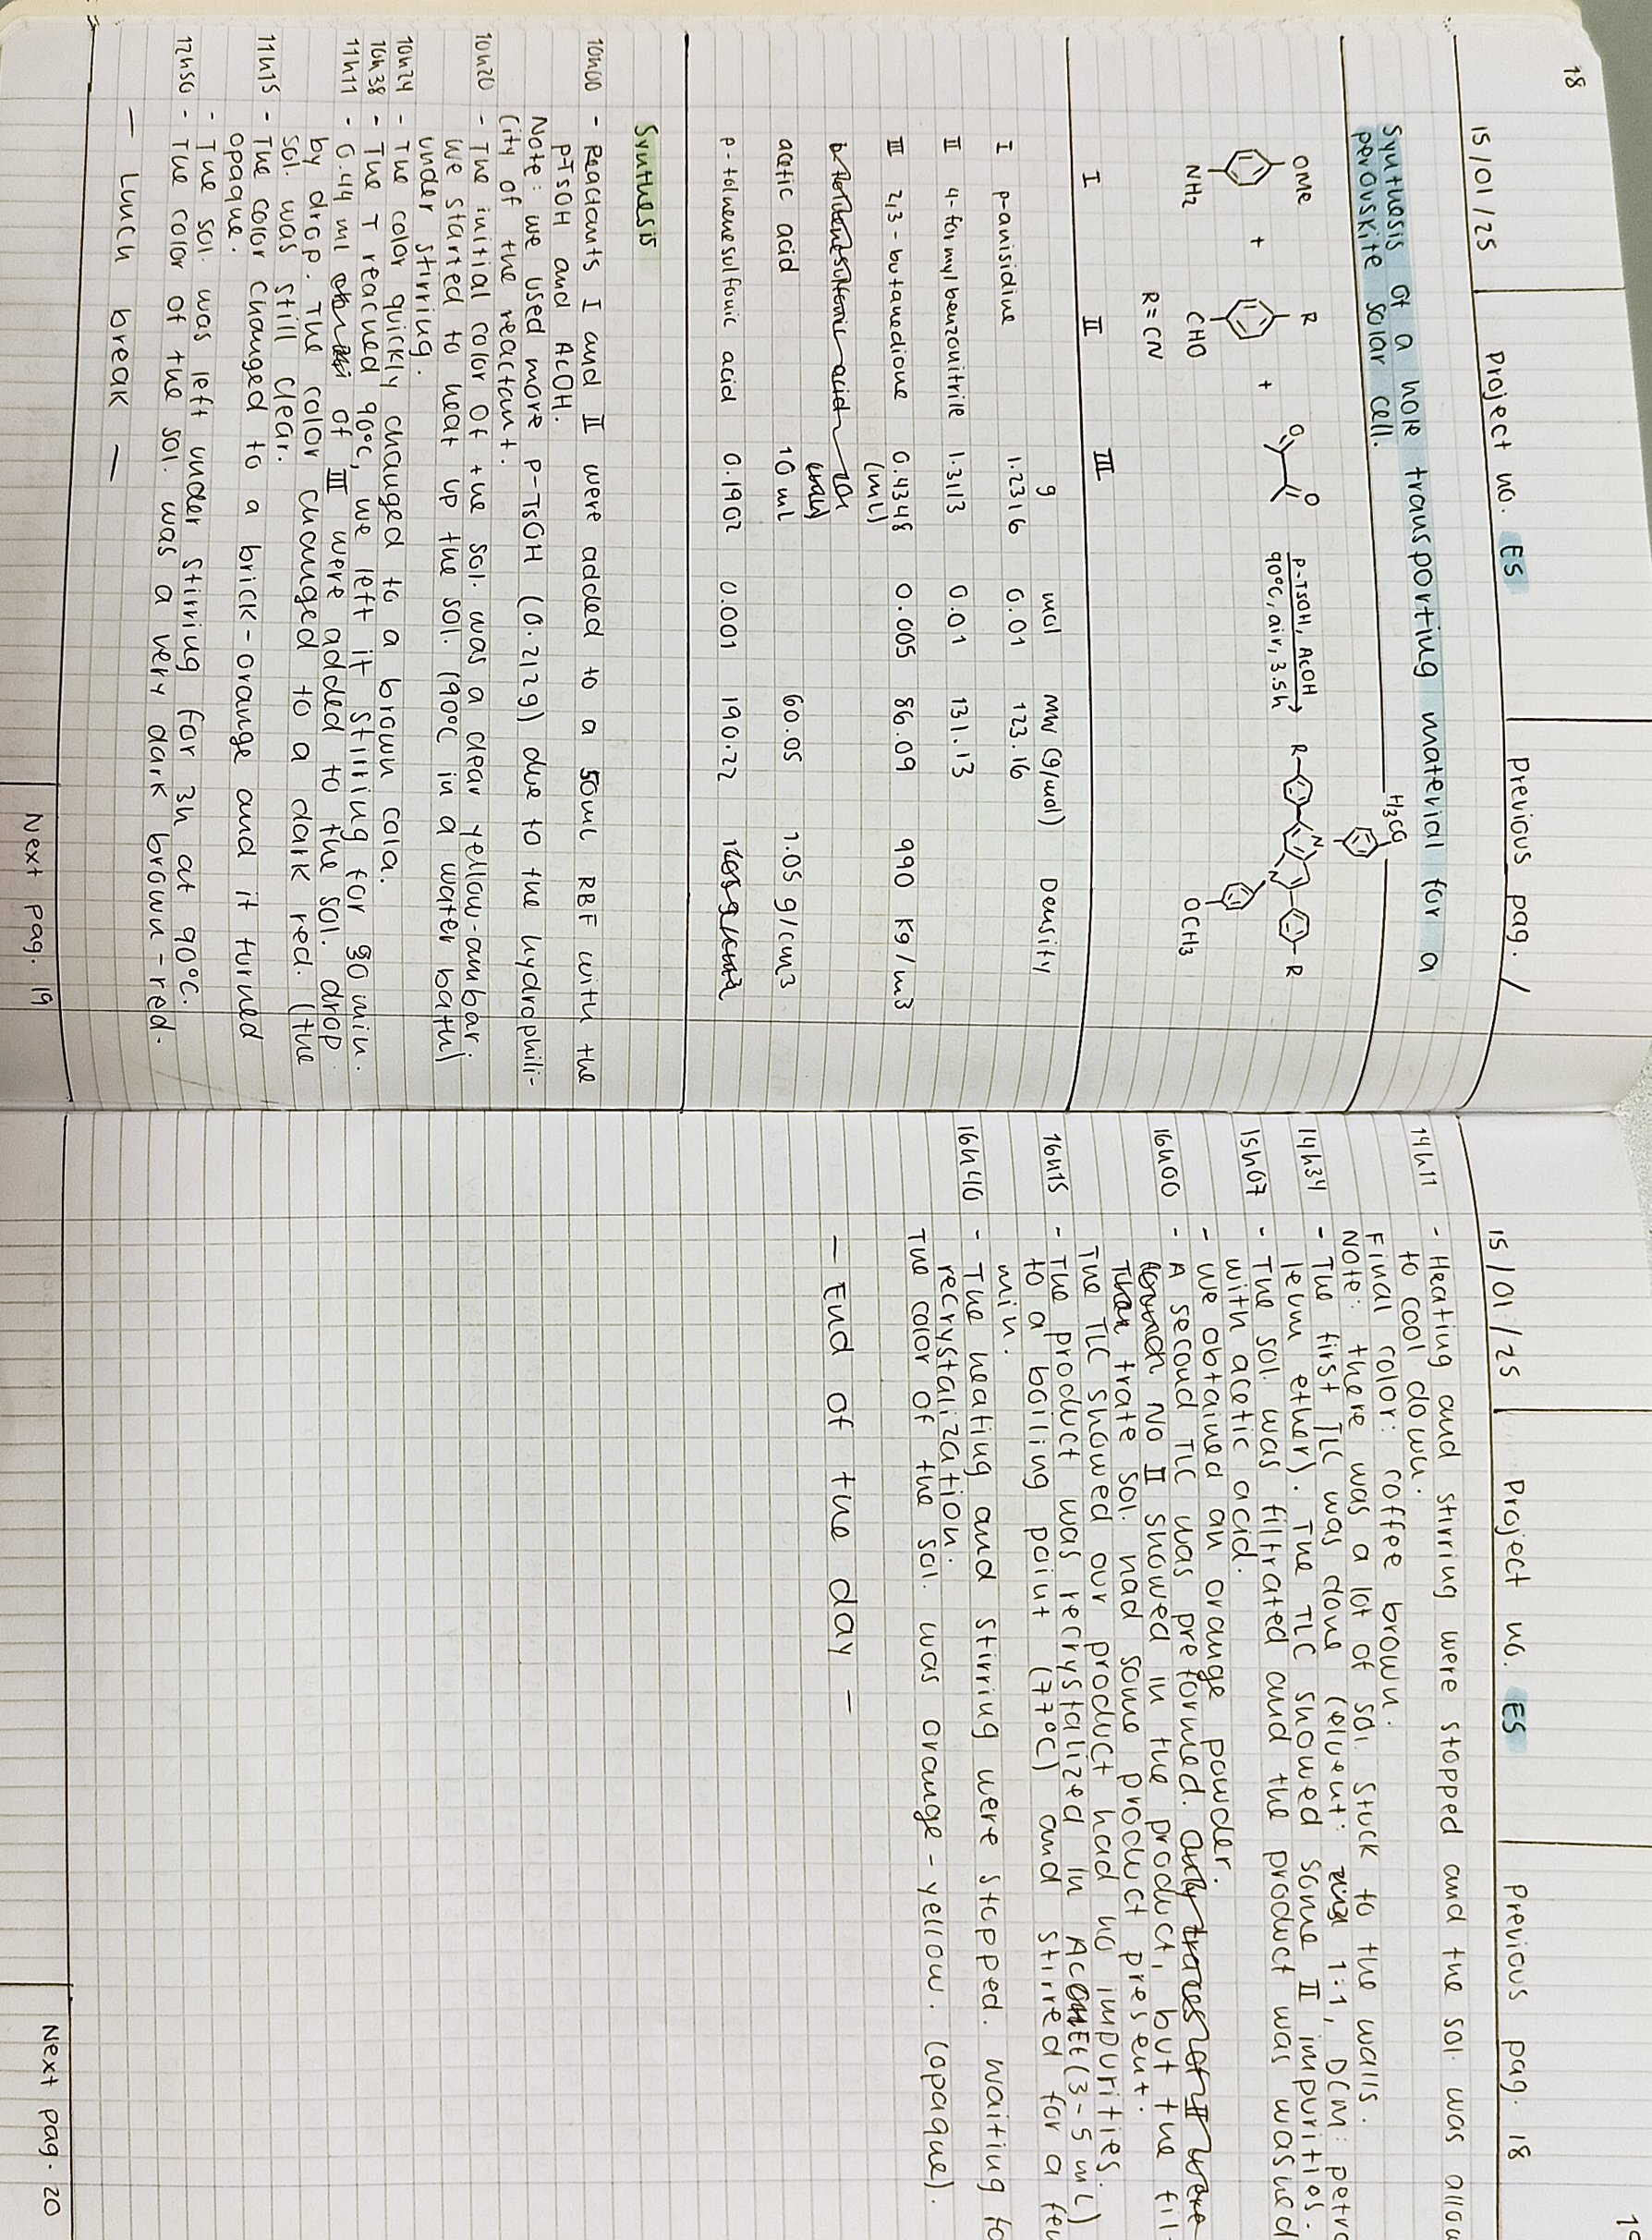
\includegraphics[width=0.6\linewidth, angle=90]{../images/compressed/IMG20250123173010.jpg}
\end{figure}


\subsection{Data Analysis}
\begin{figure}[H]
	\centering
	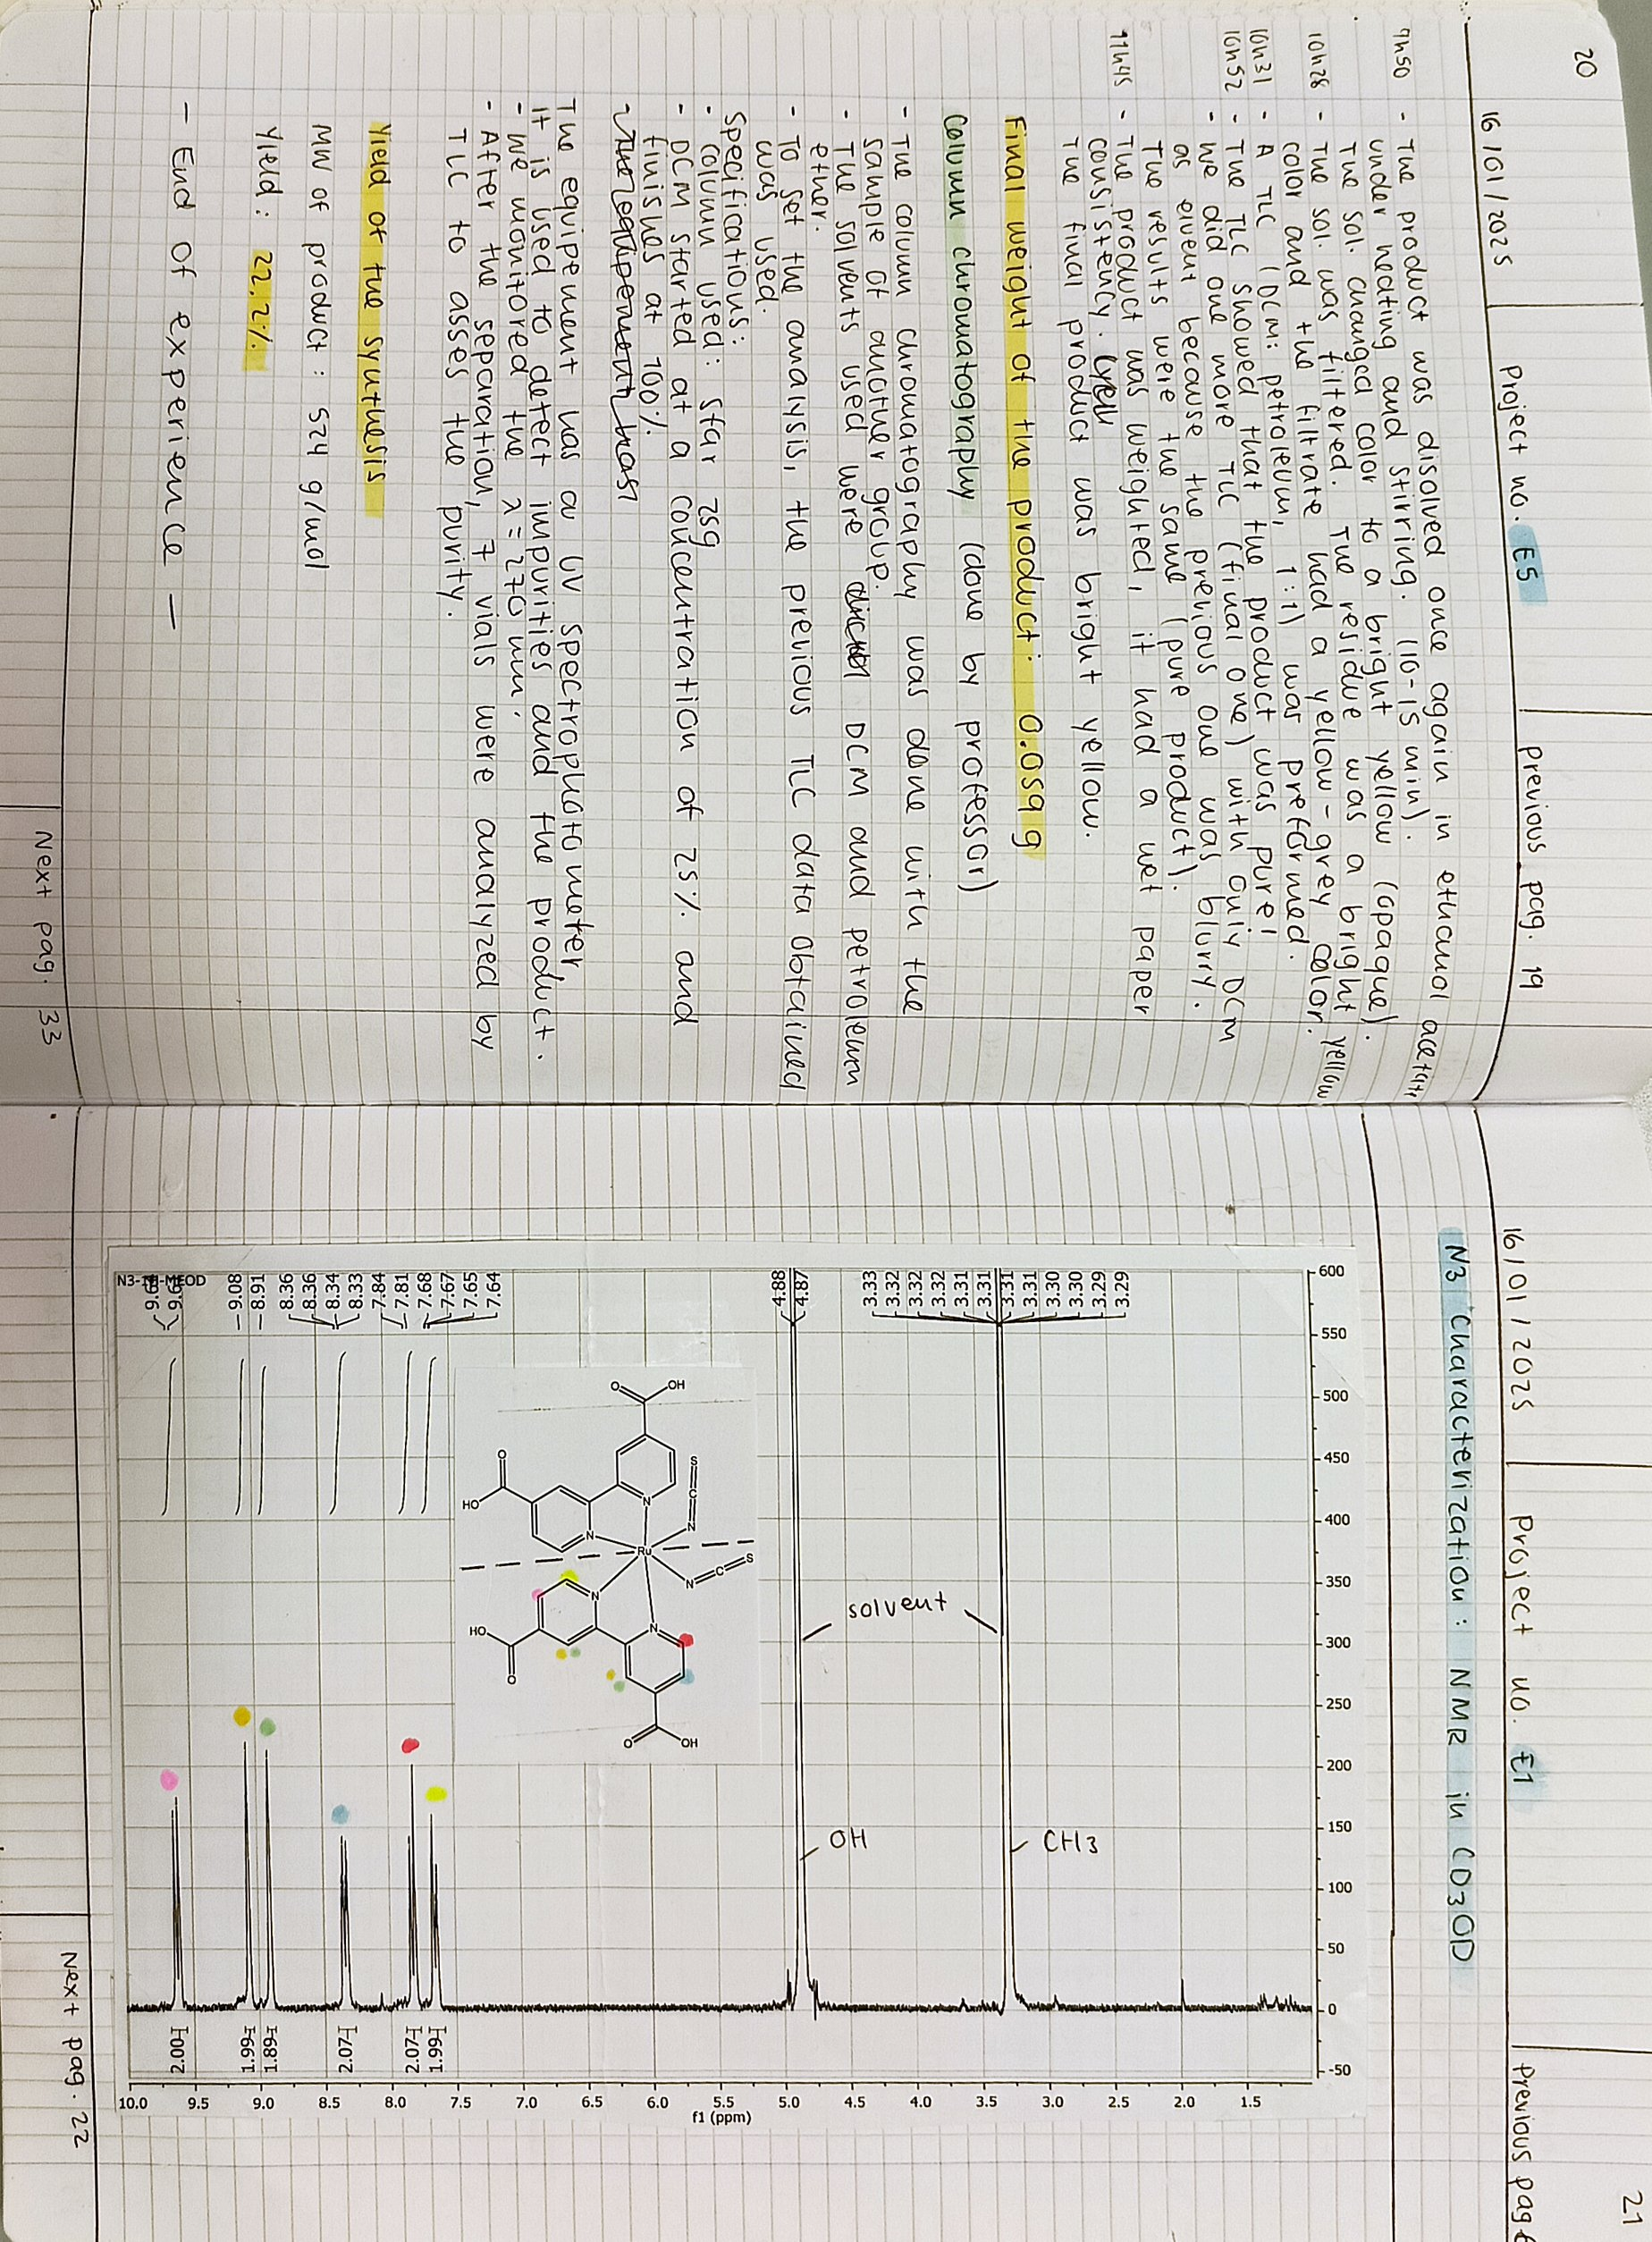
\includegraphics[width=0.6\linewidth, angle=90]{../images/compressed/IMG20250123173016.jpg}
\end{figure}
\begin{figure}[H]
	\centering
	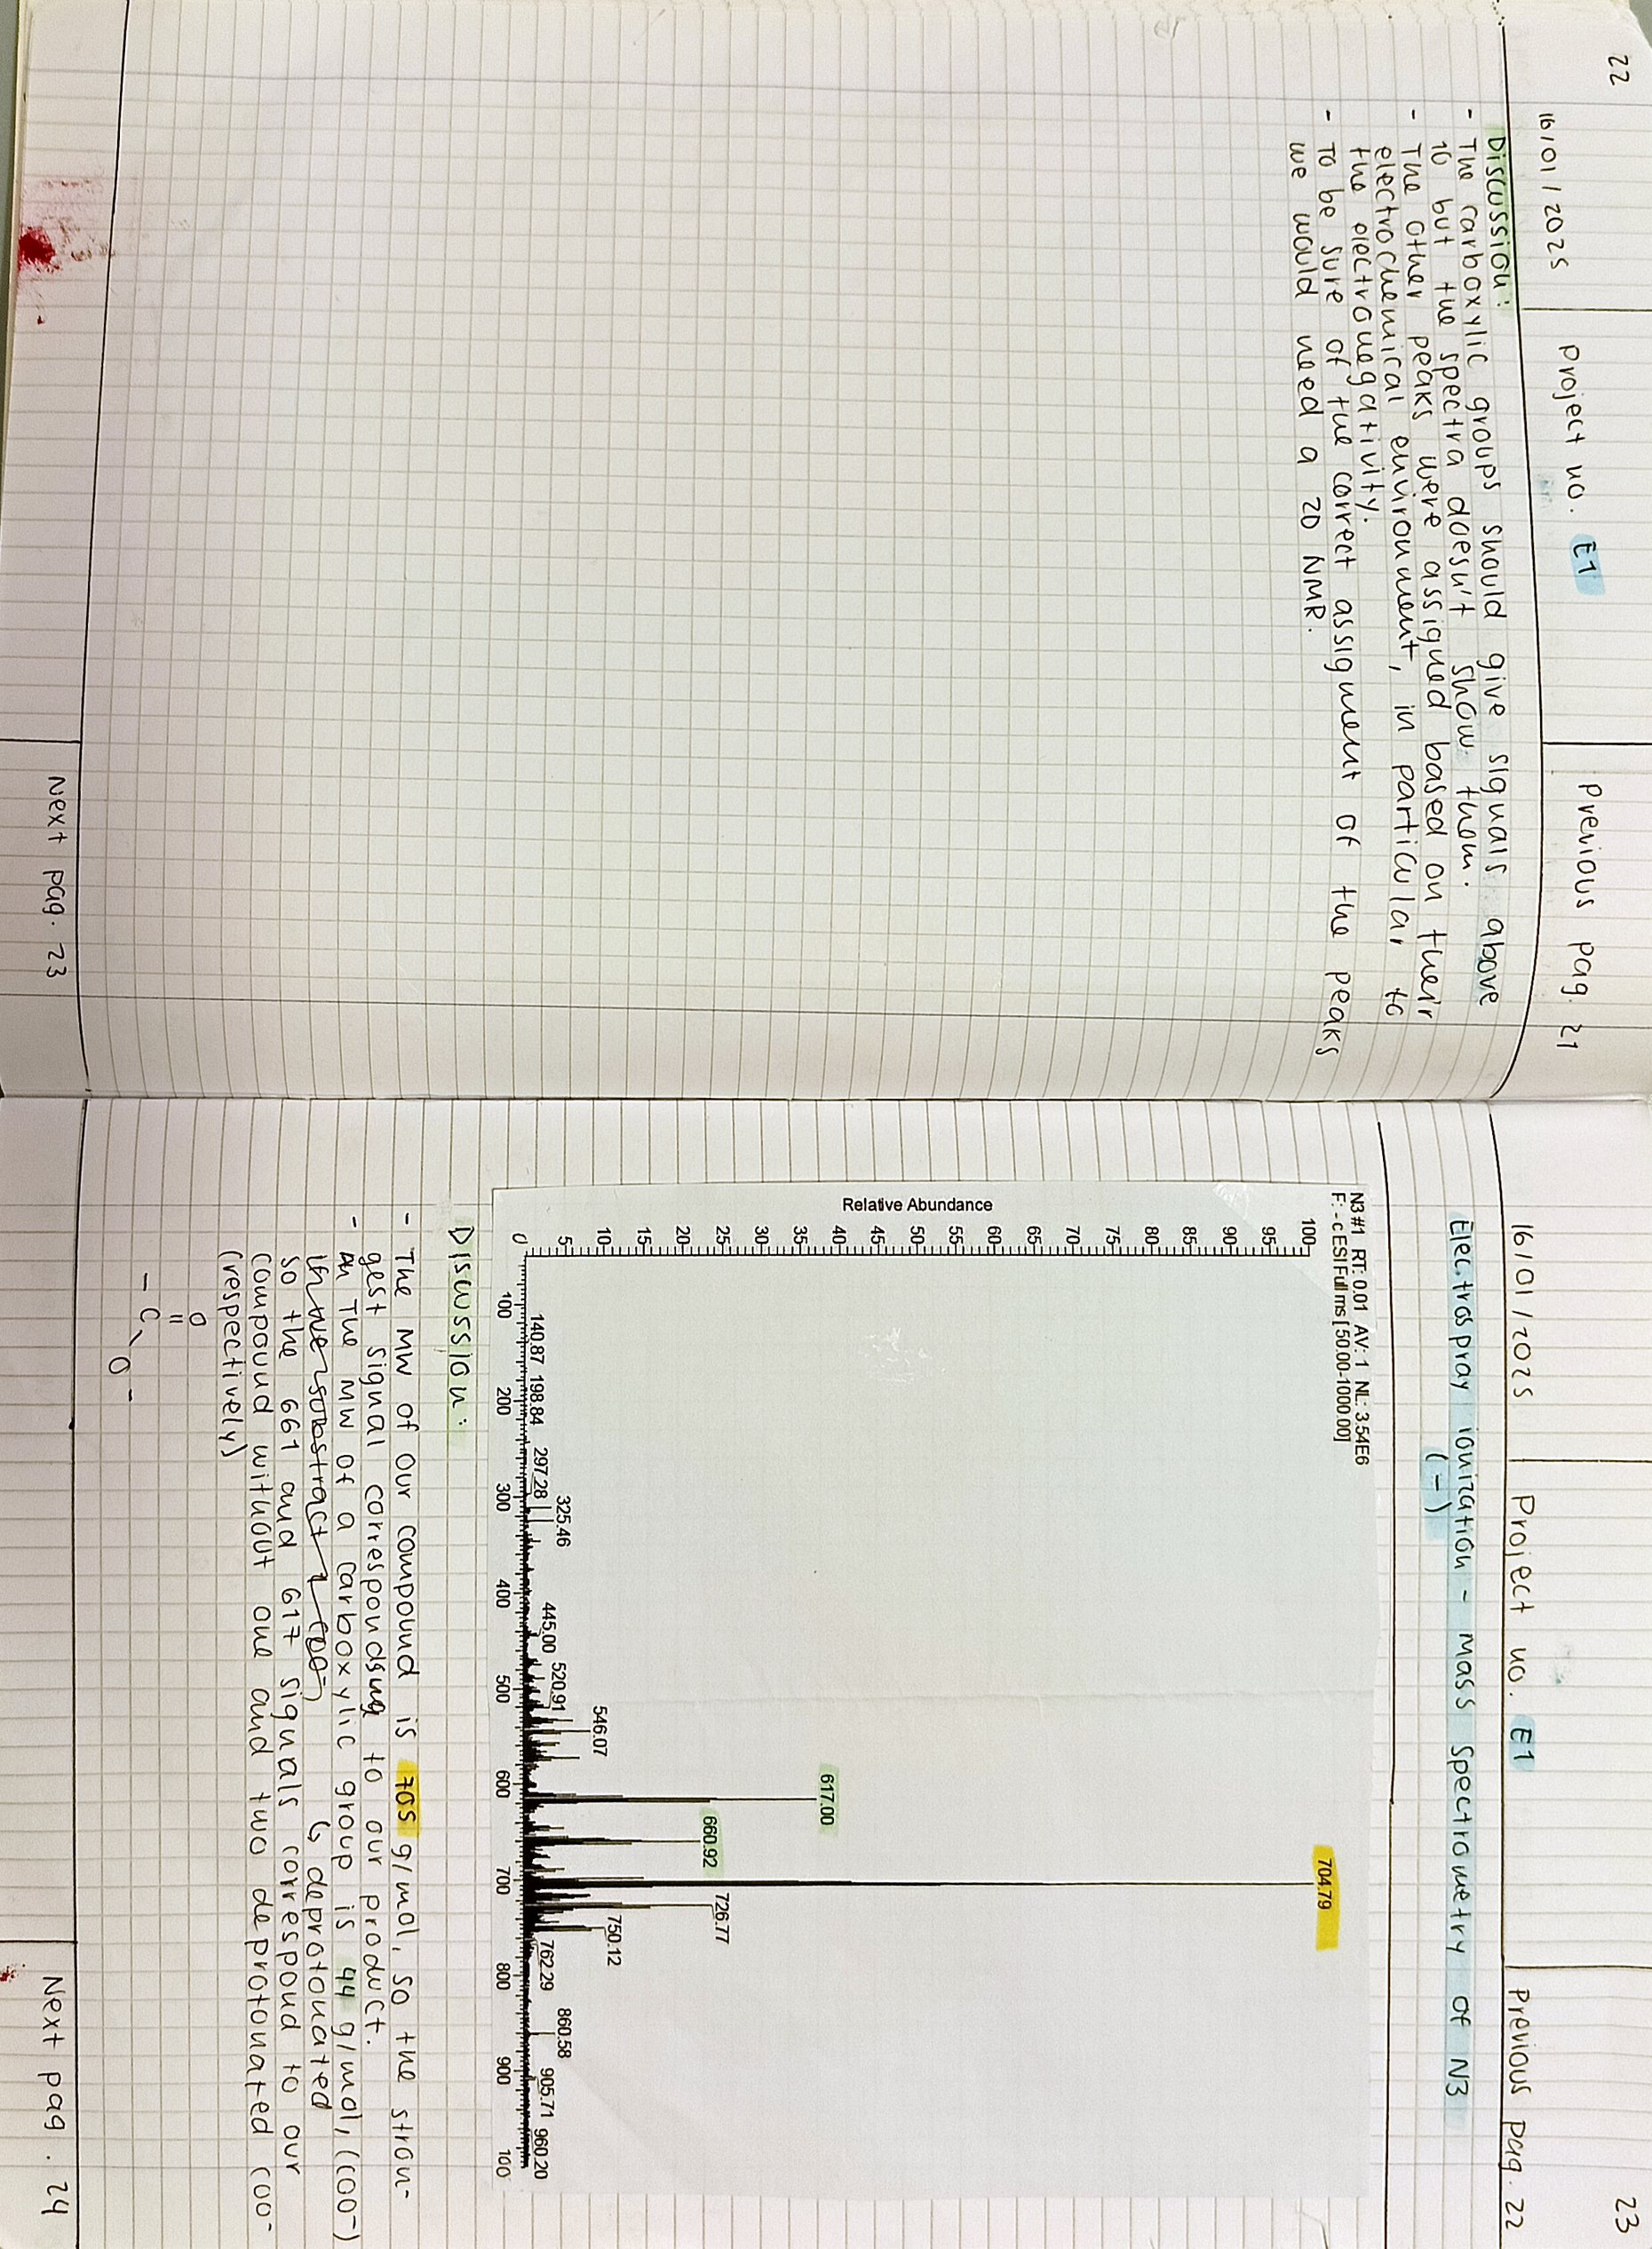
\includegraphics[width=0.6\linewidth, angle=90]{../images/compressed/IMG20250123173022.jpg}
\end{figure}
\begin{figure}[H]
	\centering
	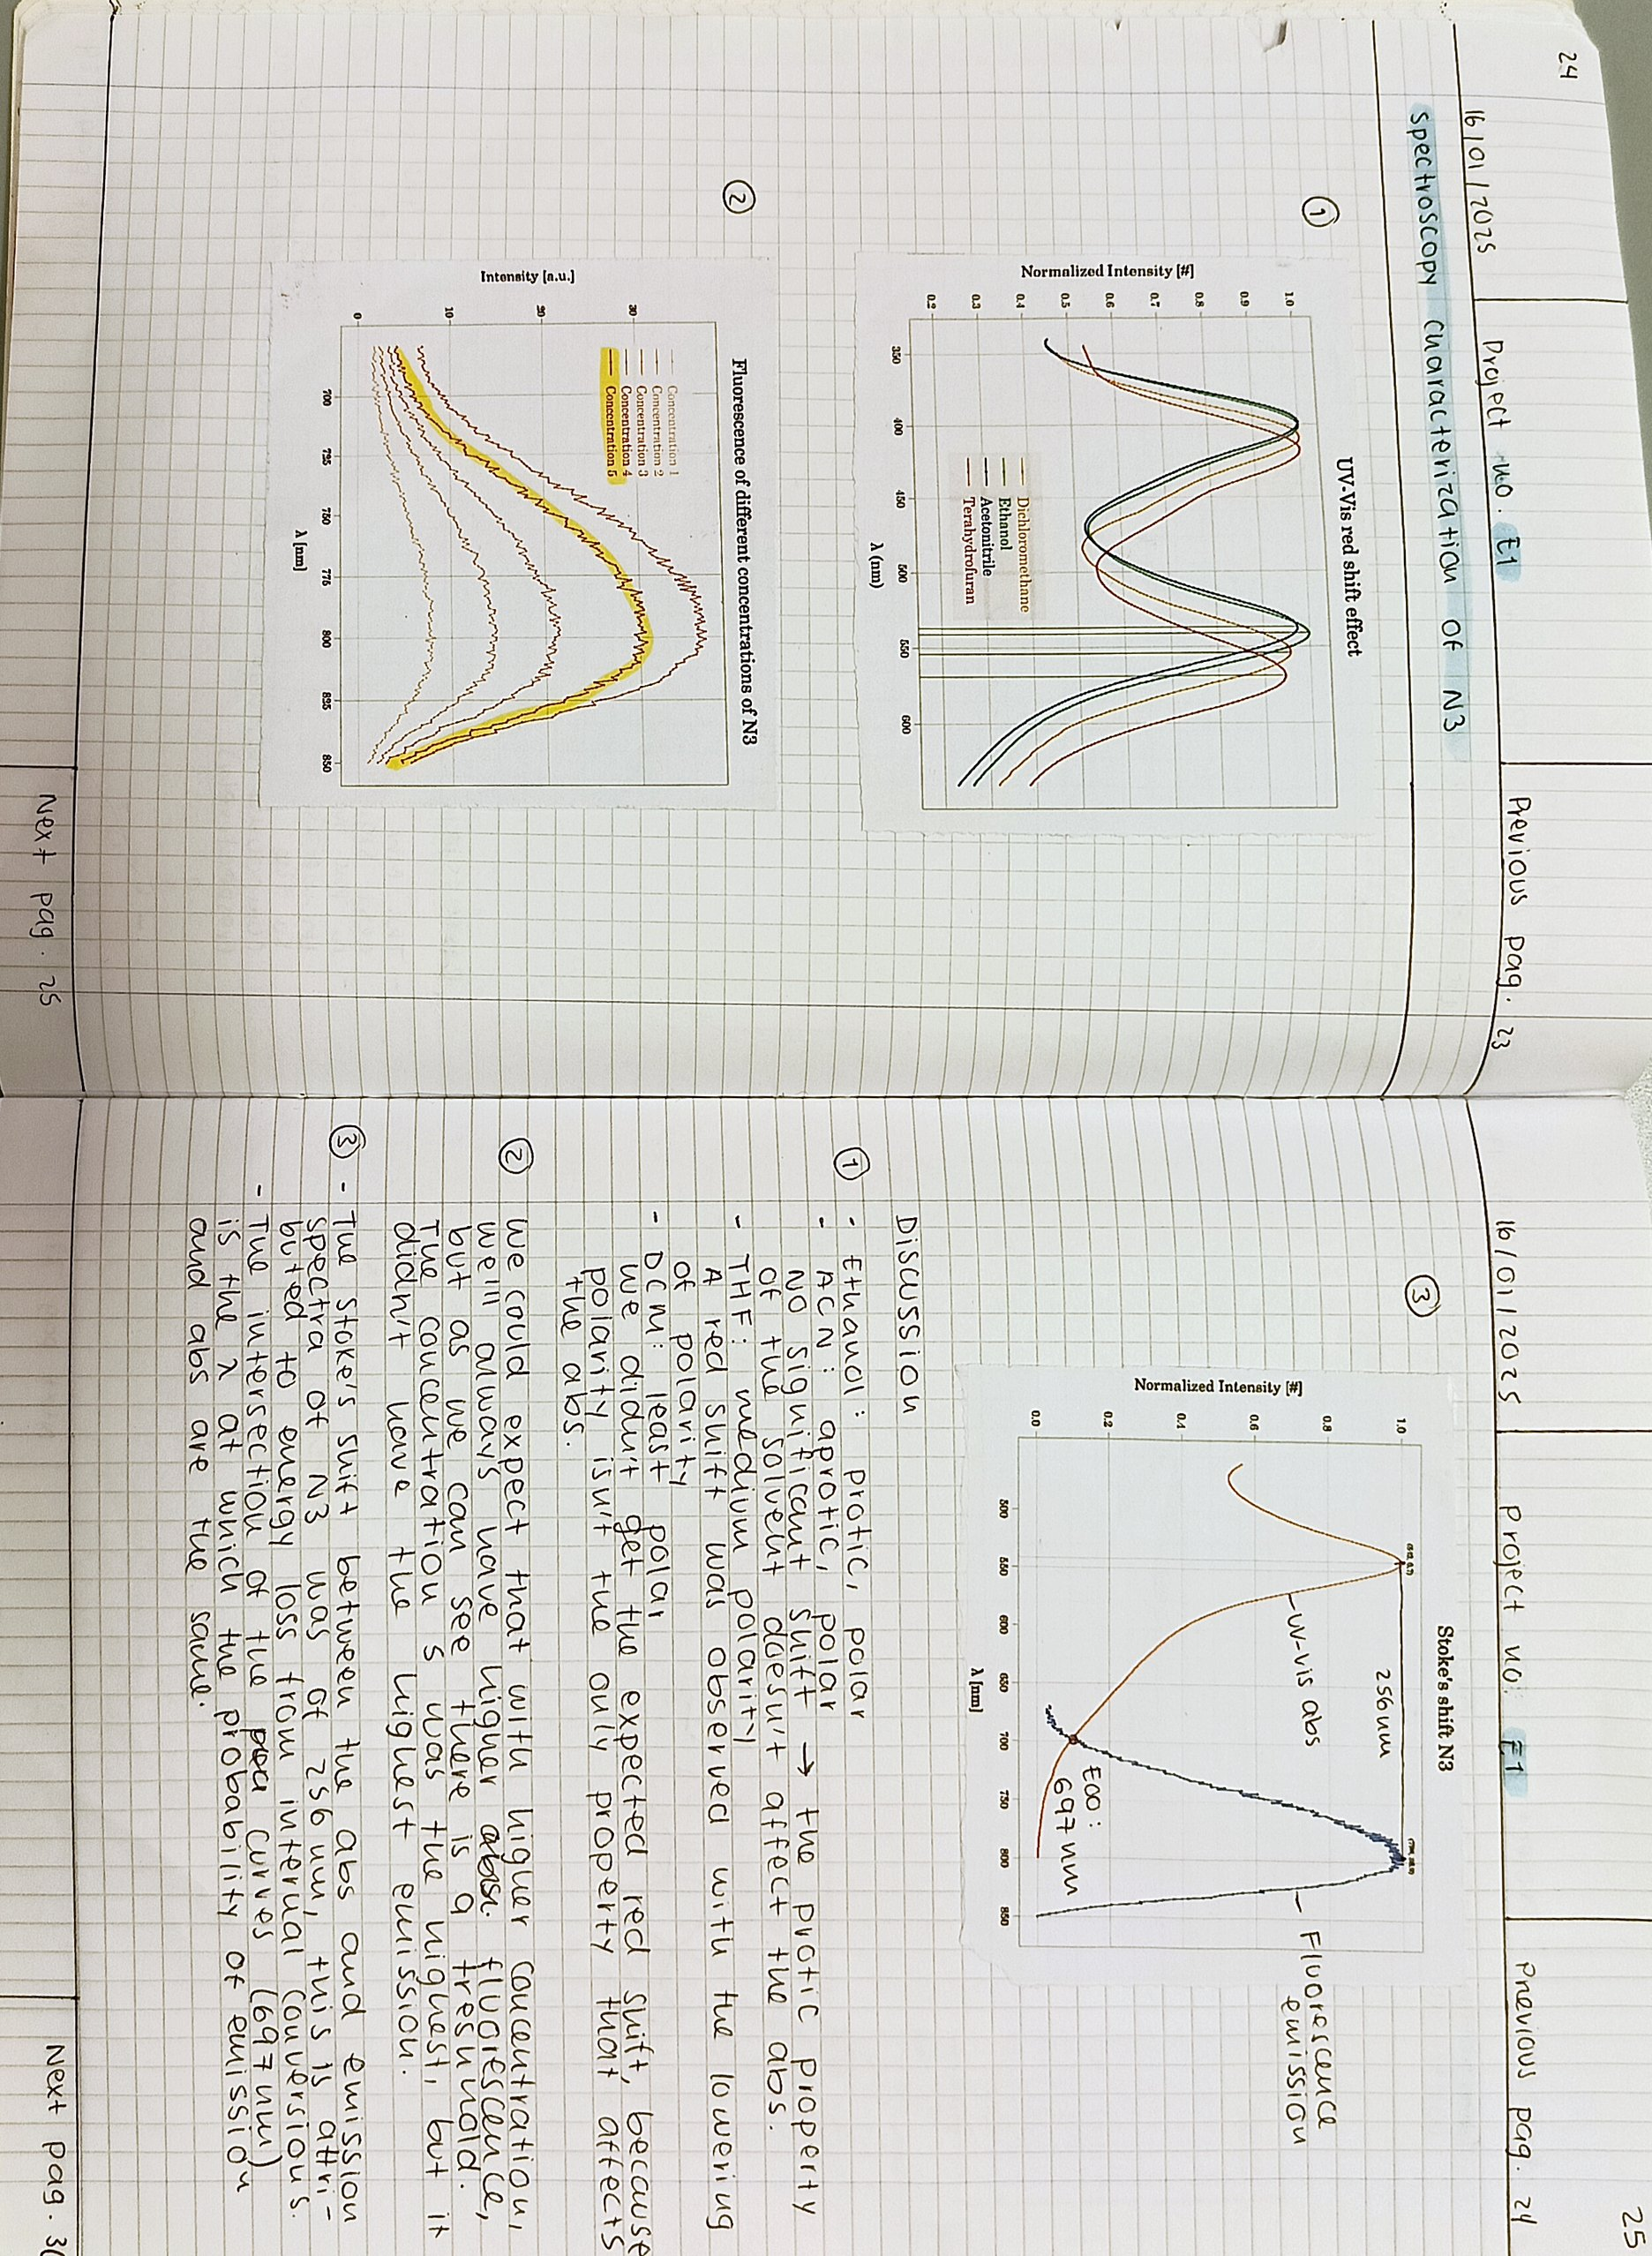
\includegraphics[width=0.6\linewidth, angle=90]{../images/compressed/IMG20250123173027.jpg}
\end{figure}
\begin{figure}[H]
	\centering
	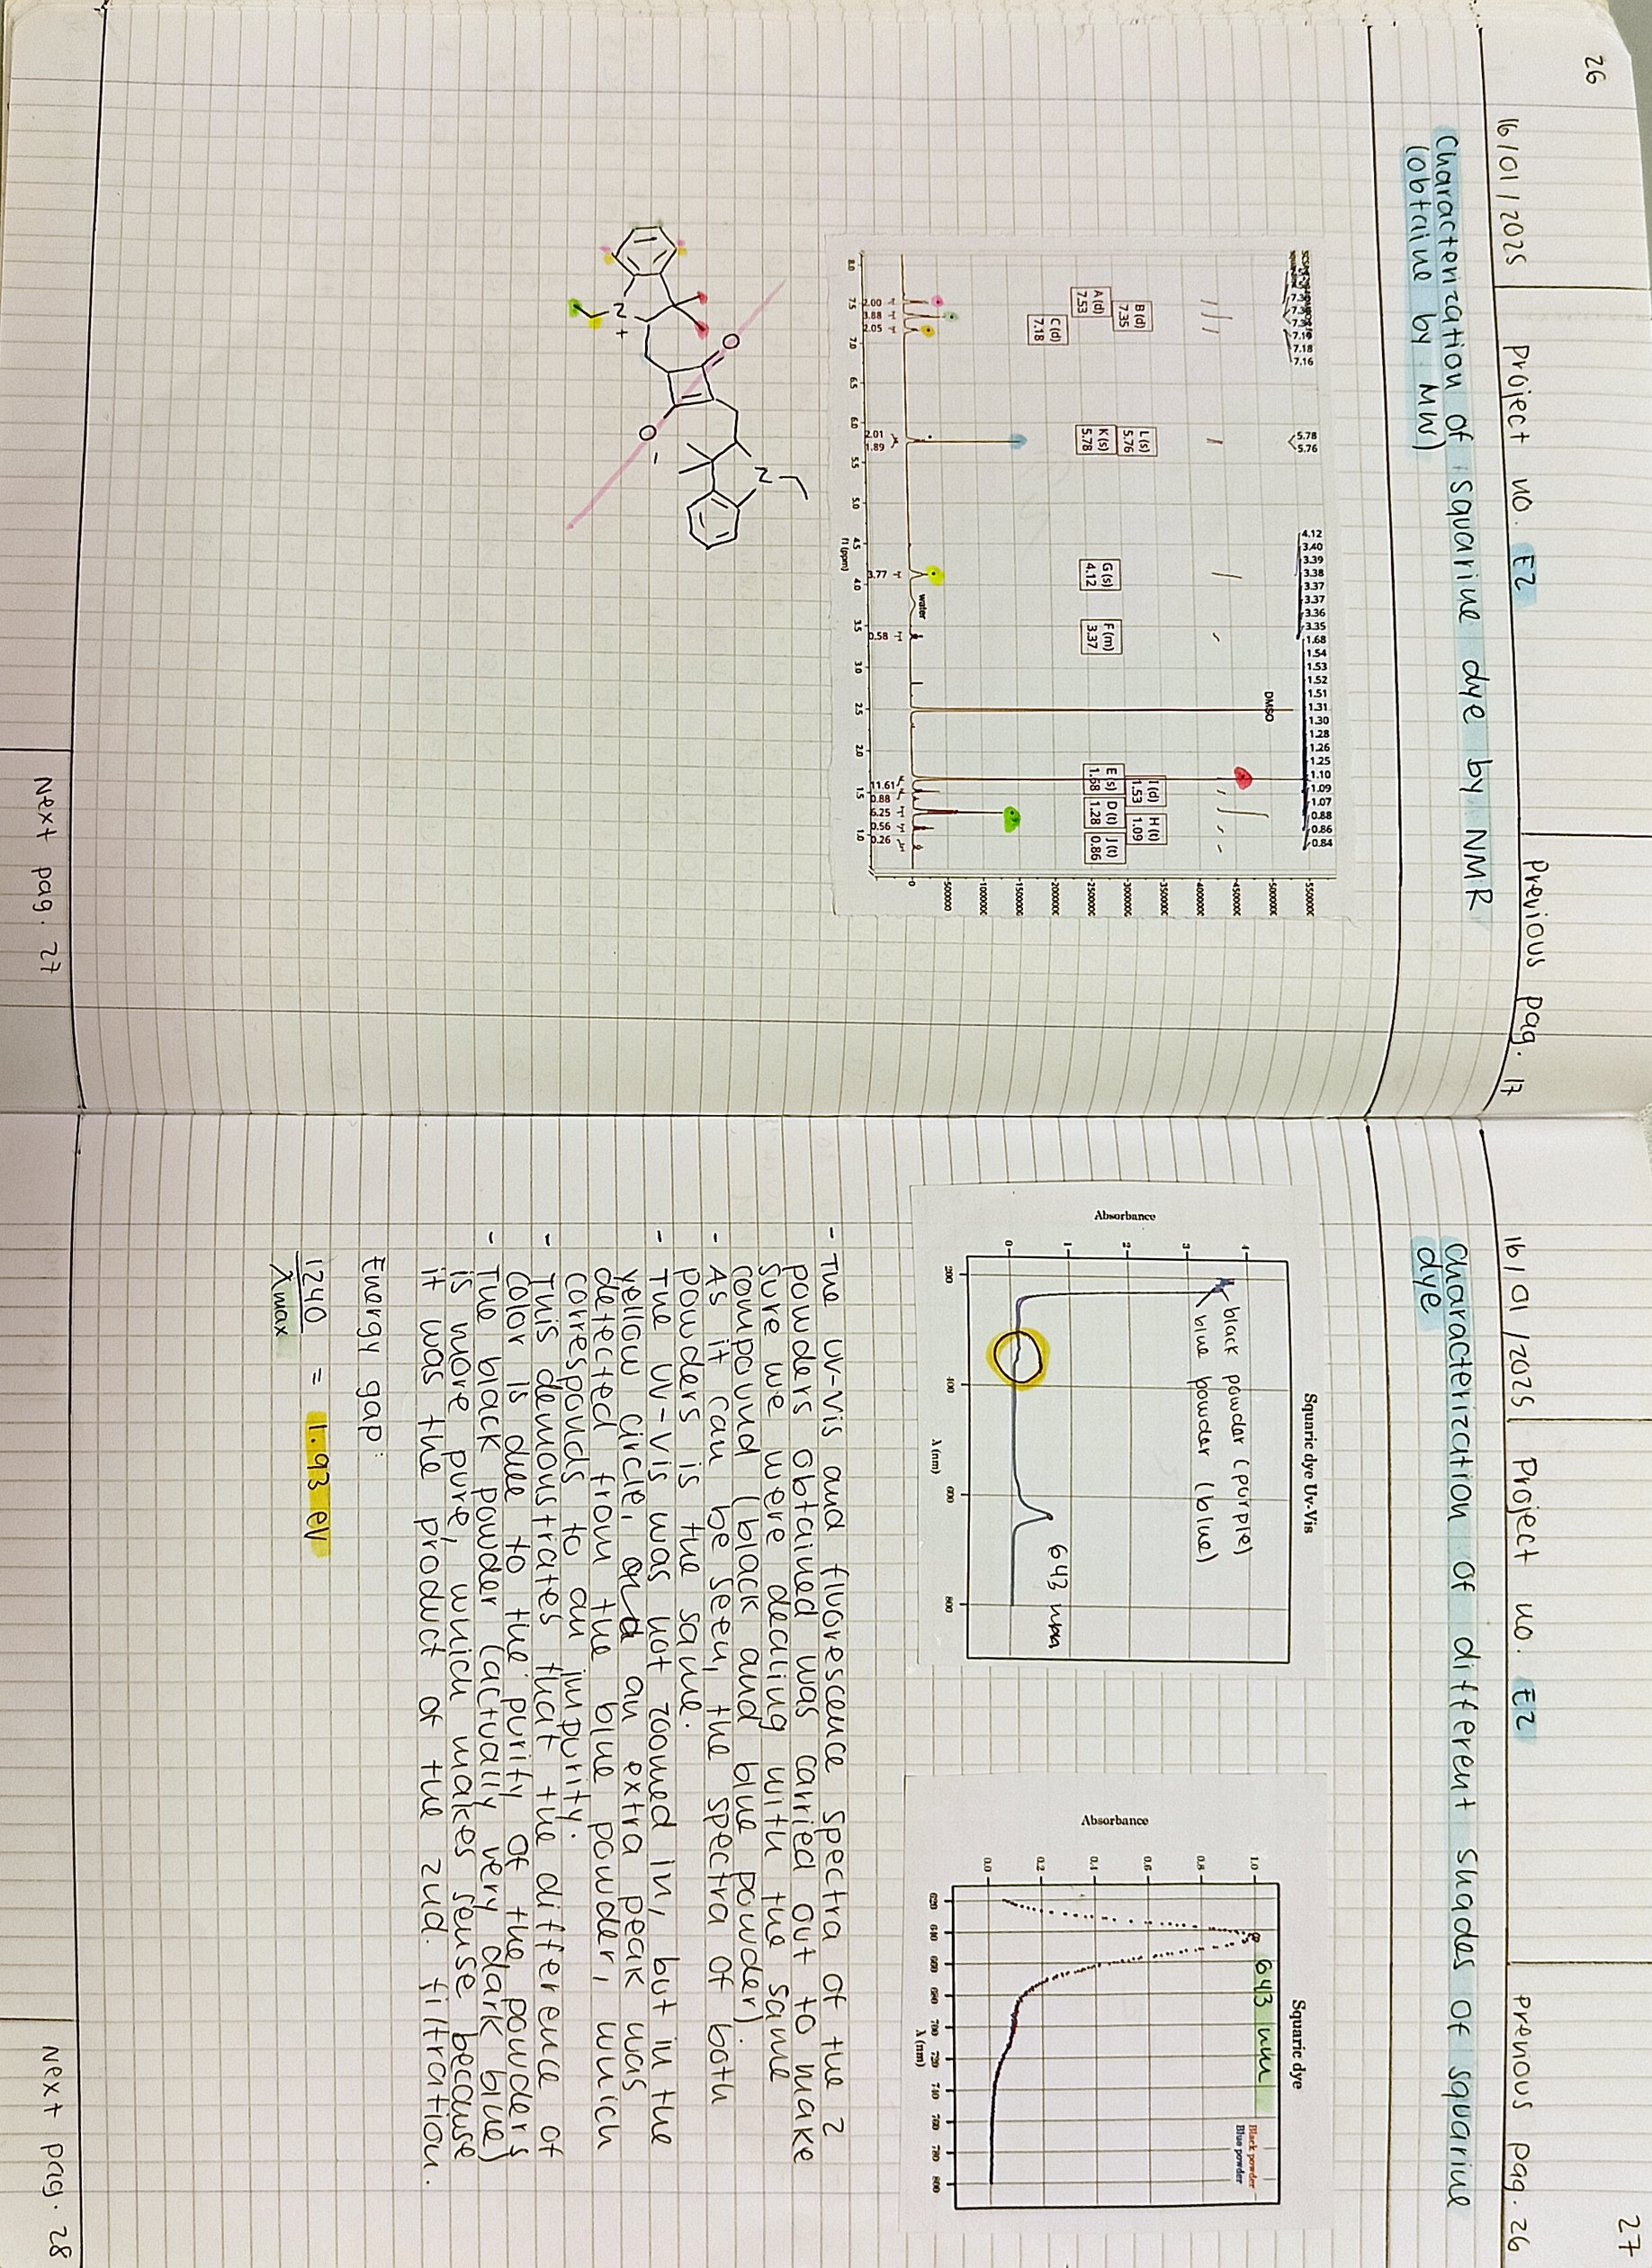
\includegraphics[width=0.6\linewidth, angle=90]{../images/compressed/IMG20250123173032.jpg}
\end{figure}
\begin{figure}[H]
	\centering
	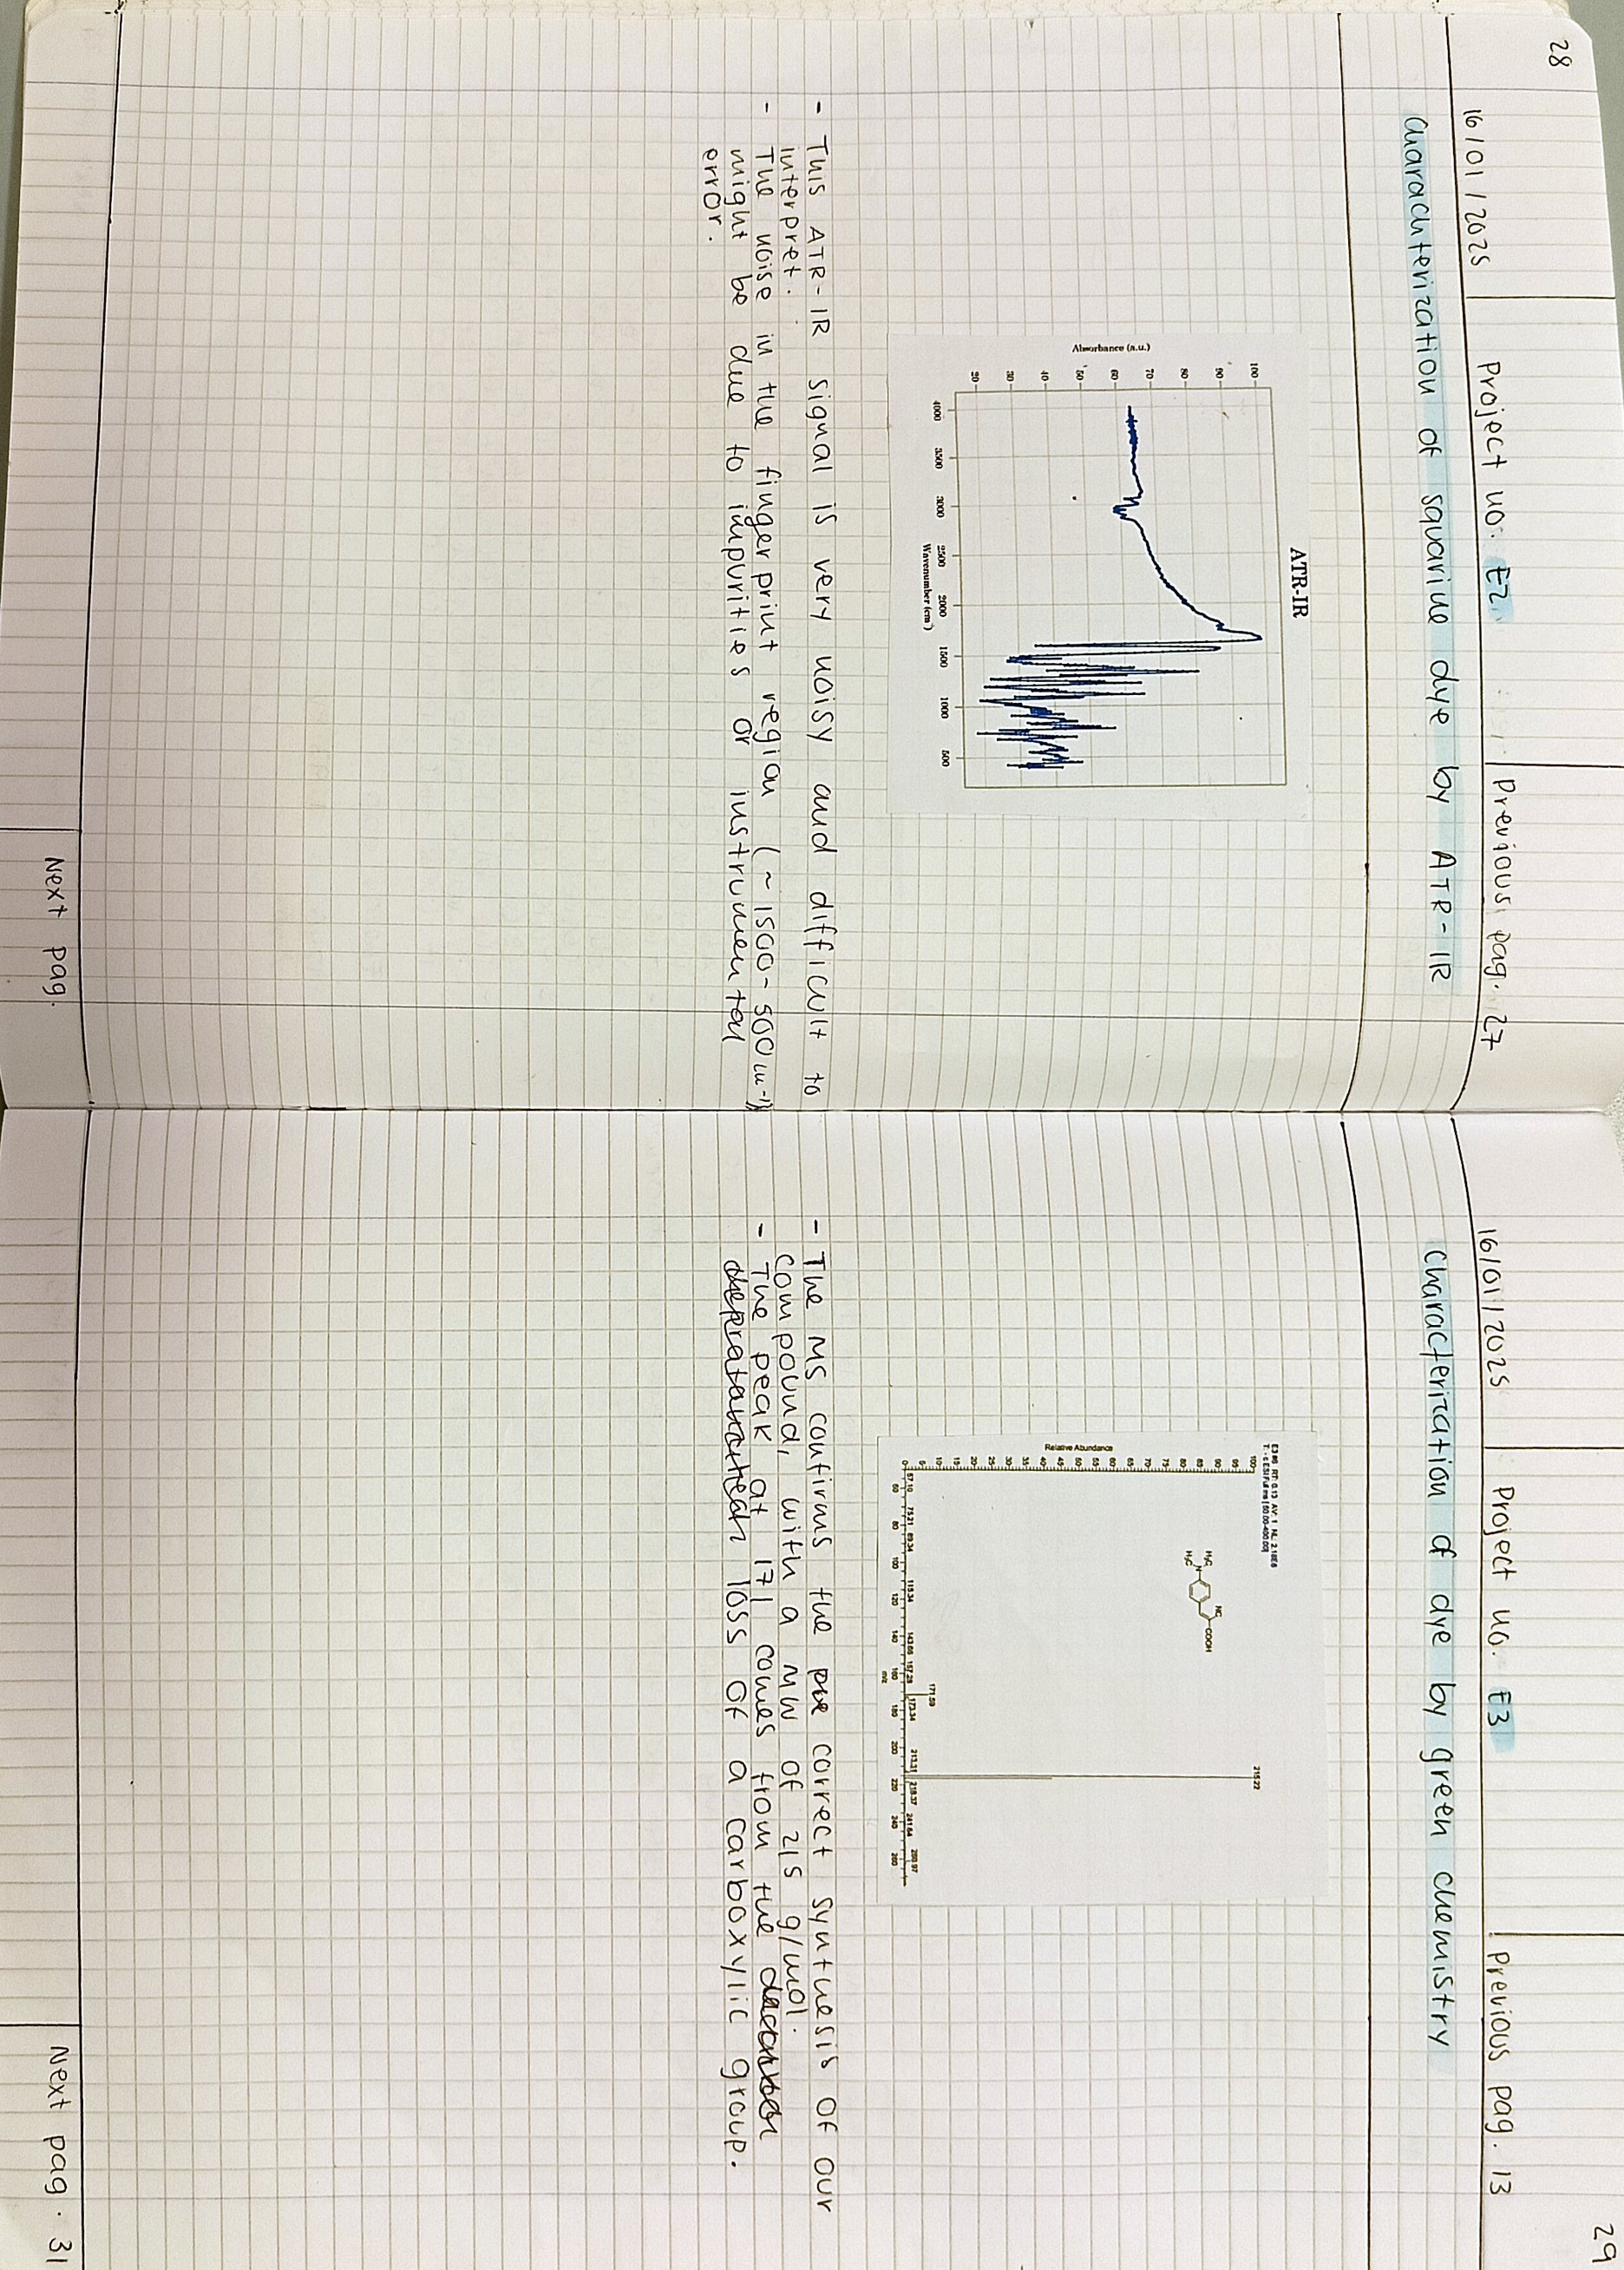
\includegraphics[width=0.6\linewidth, angle=90]{../images/compressed/IMG20250123173038.jpg}
\end{figure}
\begin{figure}[H]
	\centering
	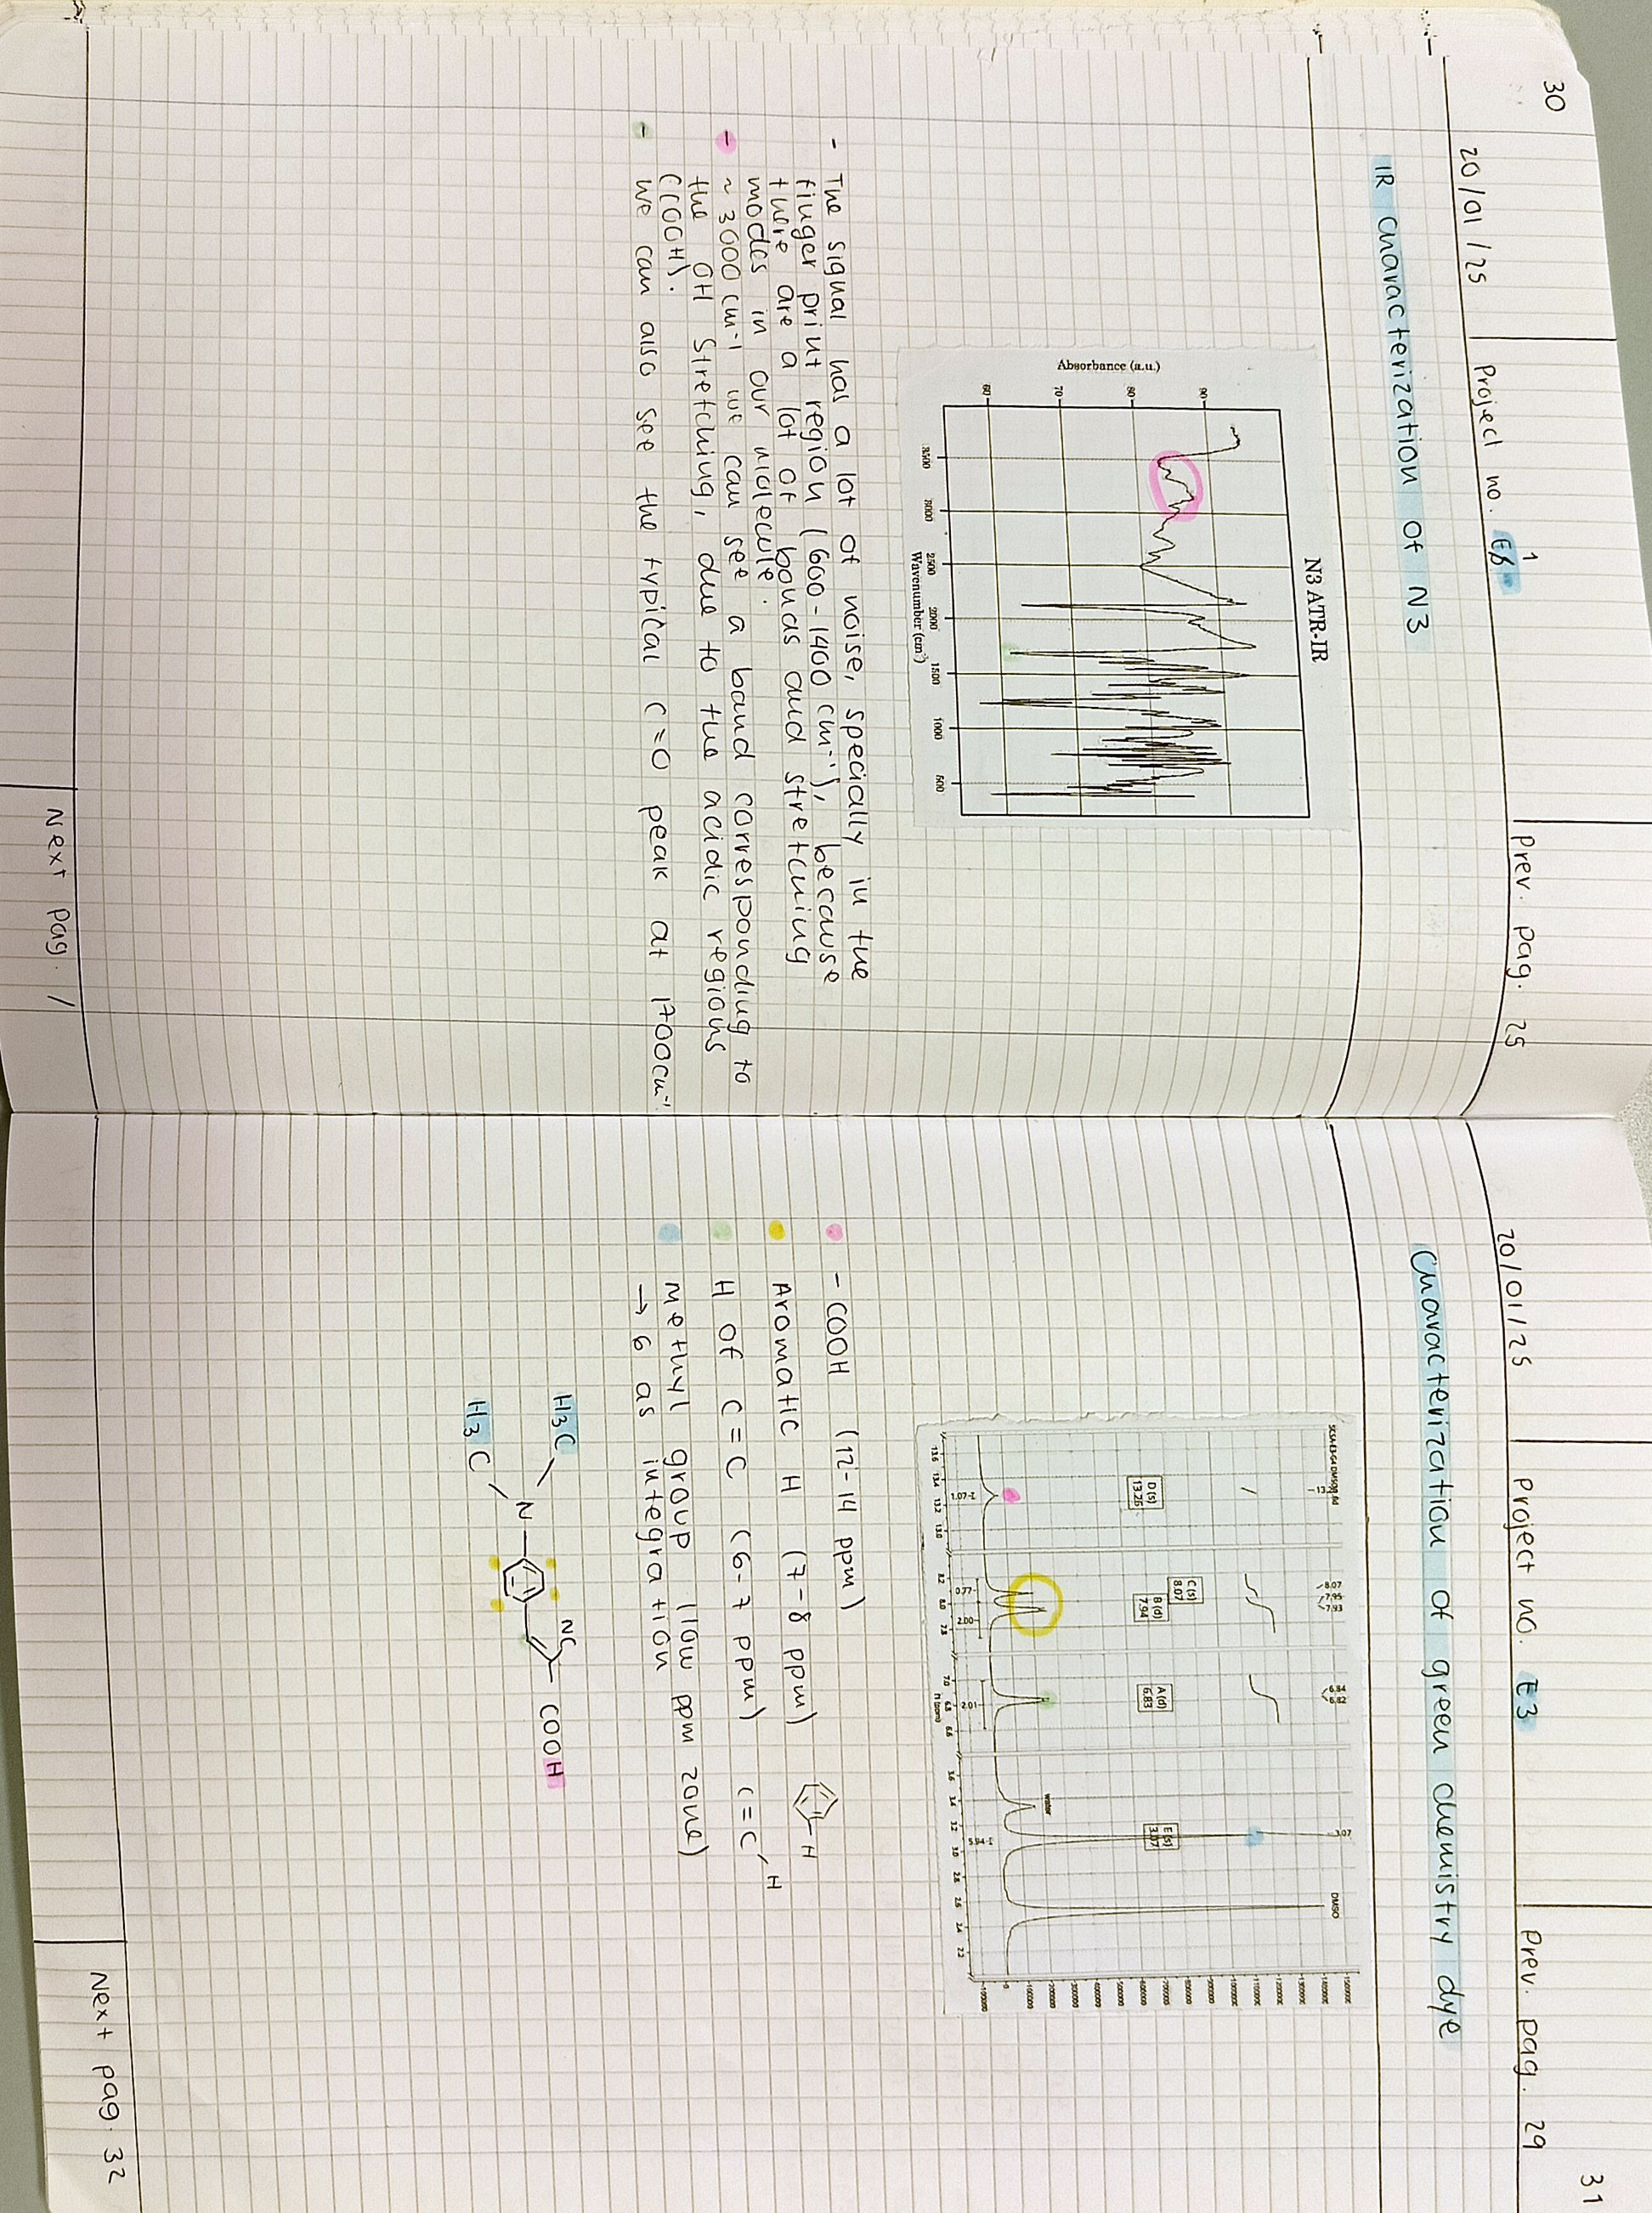
\includegraphics[width=0.6\linewidth, angle=90]{../images/compressed/IMG20250123173043.jpg}
\end{figure}
\begin{figure}[H]
	\centering
	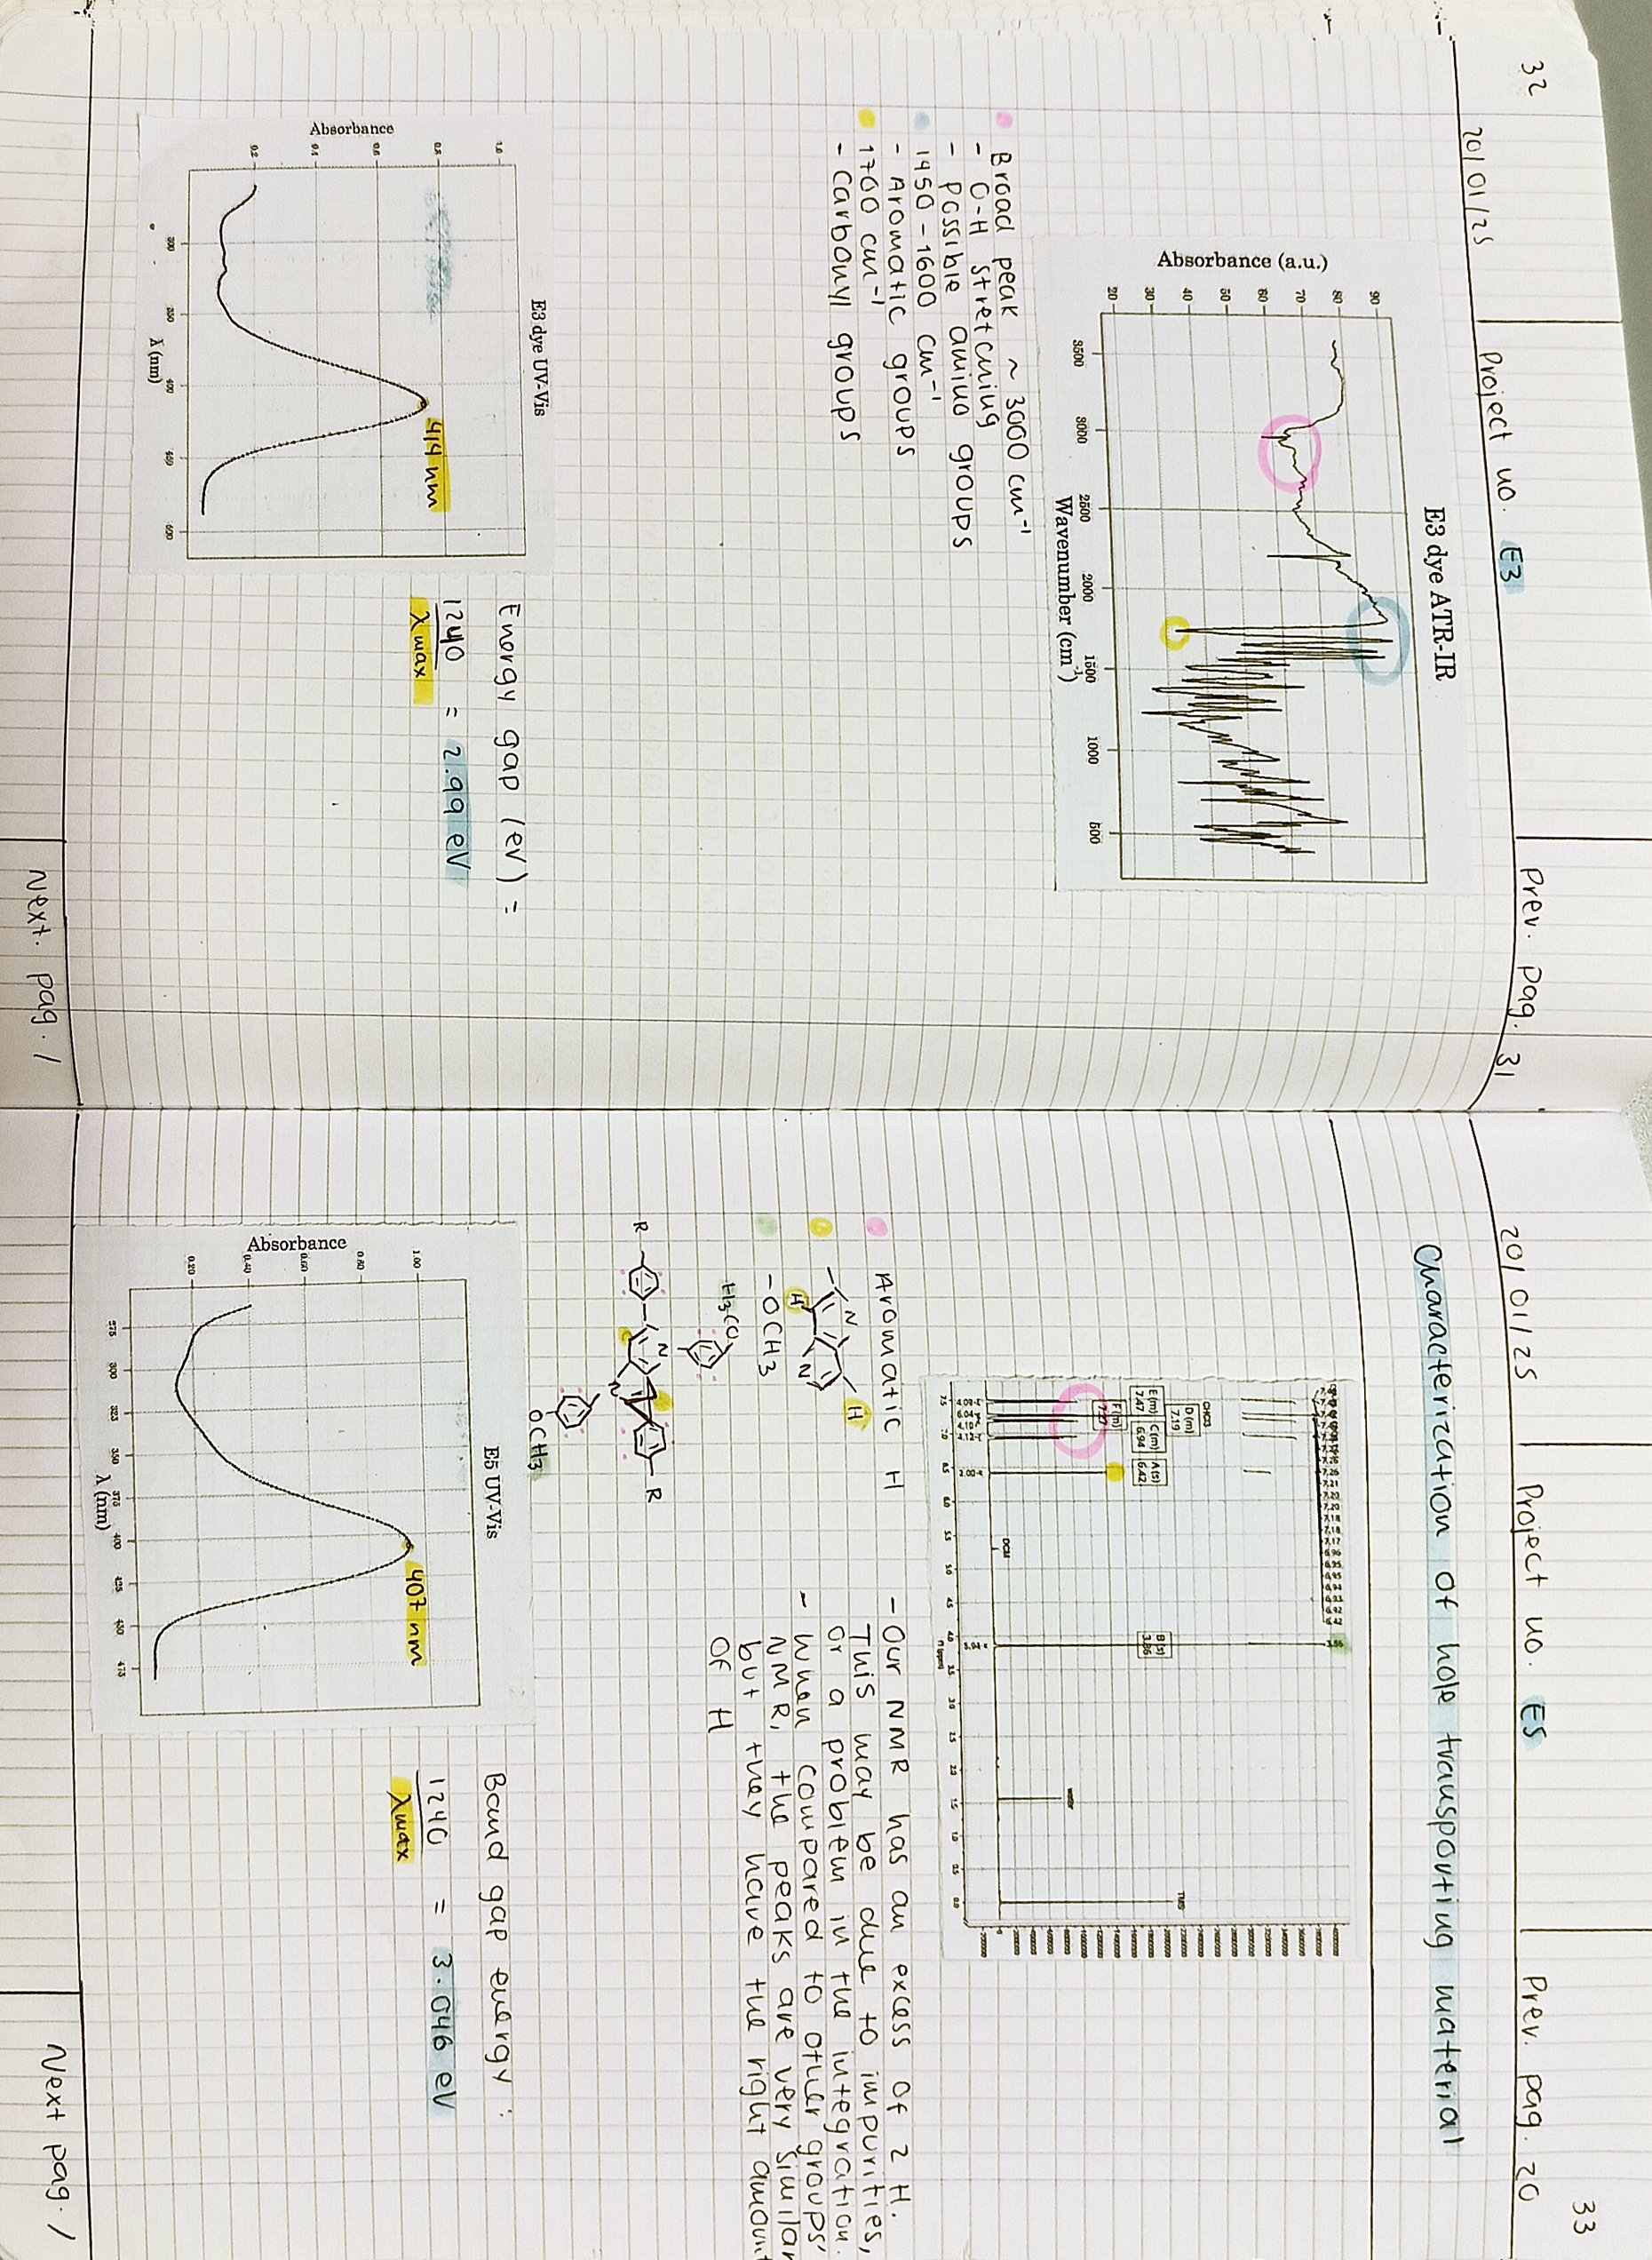
\includegraphics[width=0.6\linewidth, angle=90]{../images/compressed/IMG20250123173048.jpg}
\end{figure}


\section{Part II: Bonomo (not written in order)}


\begin{figure}[H]
	\centering
	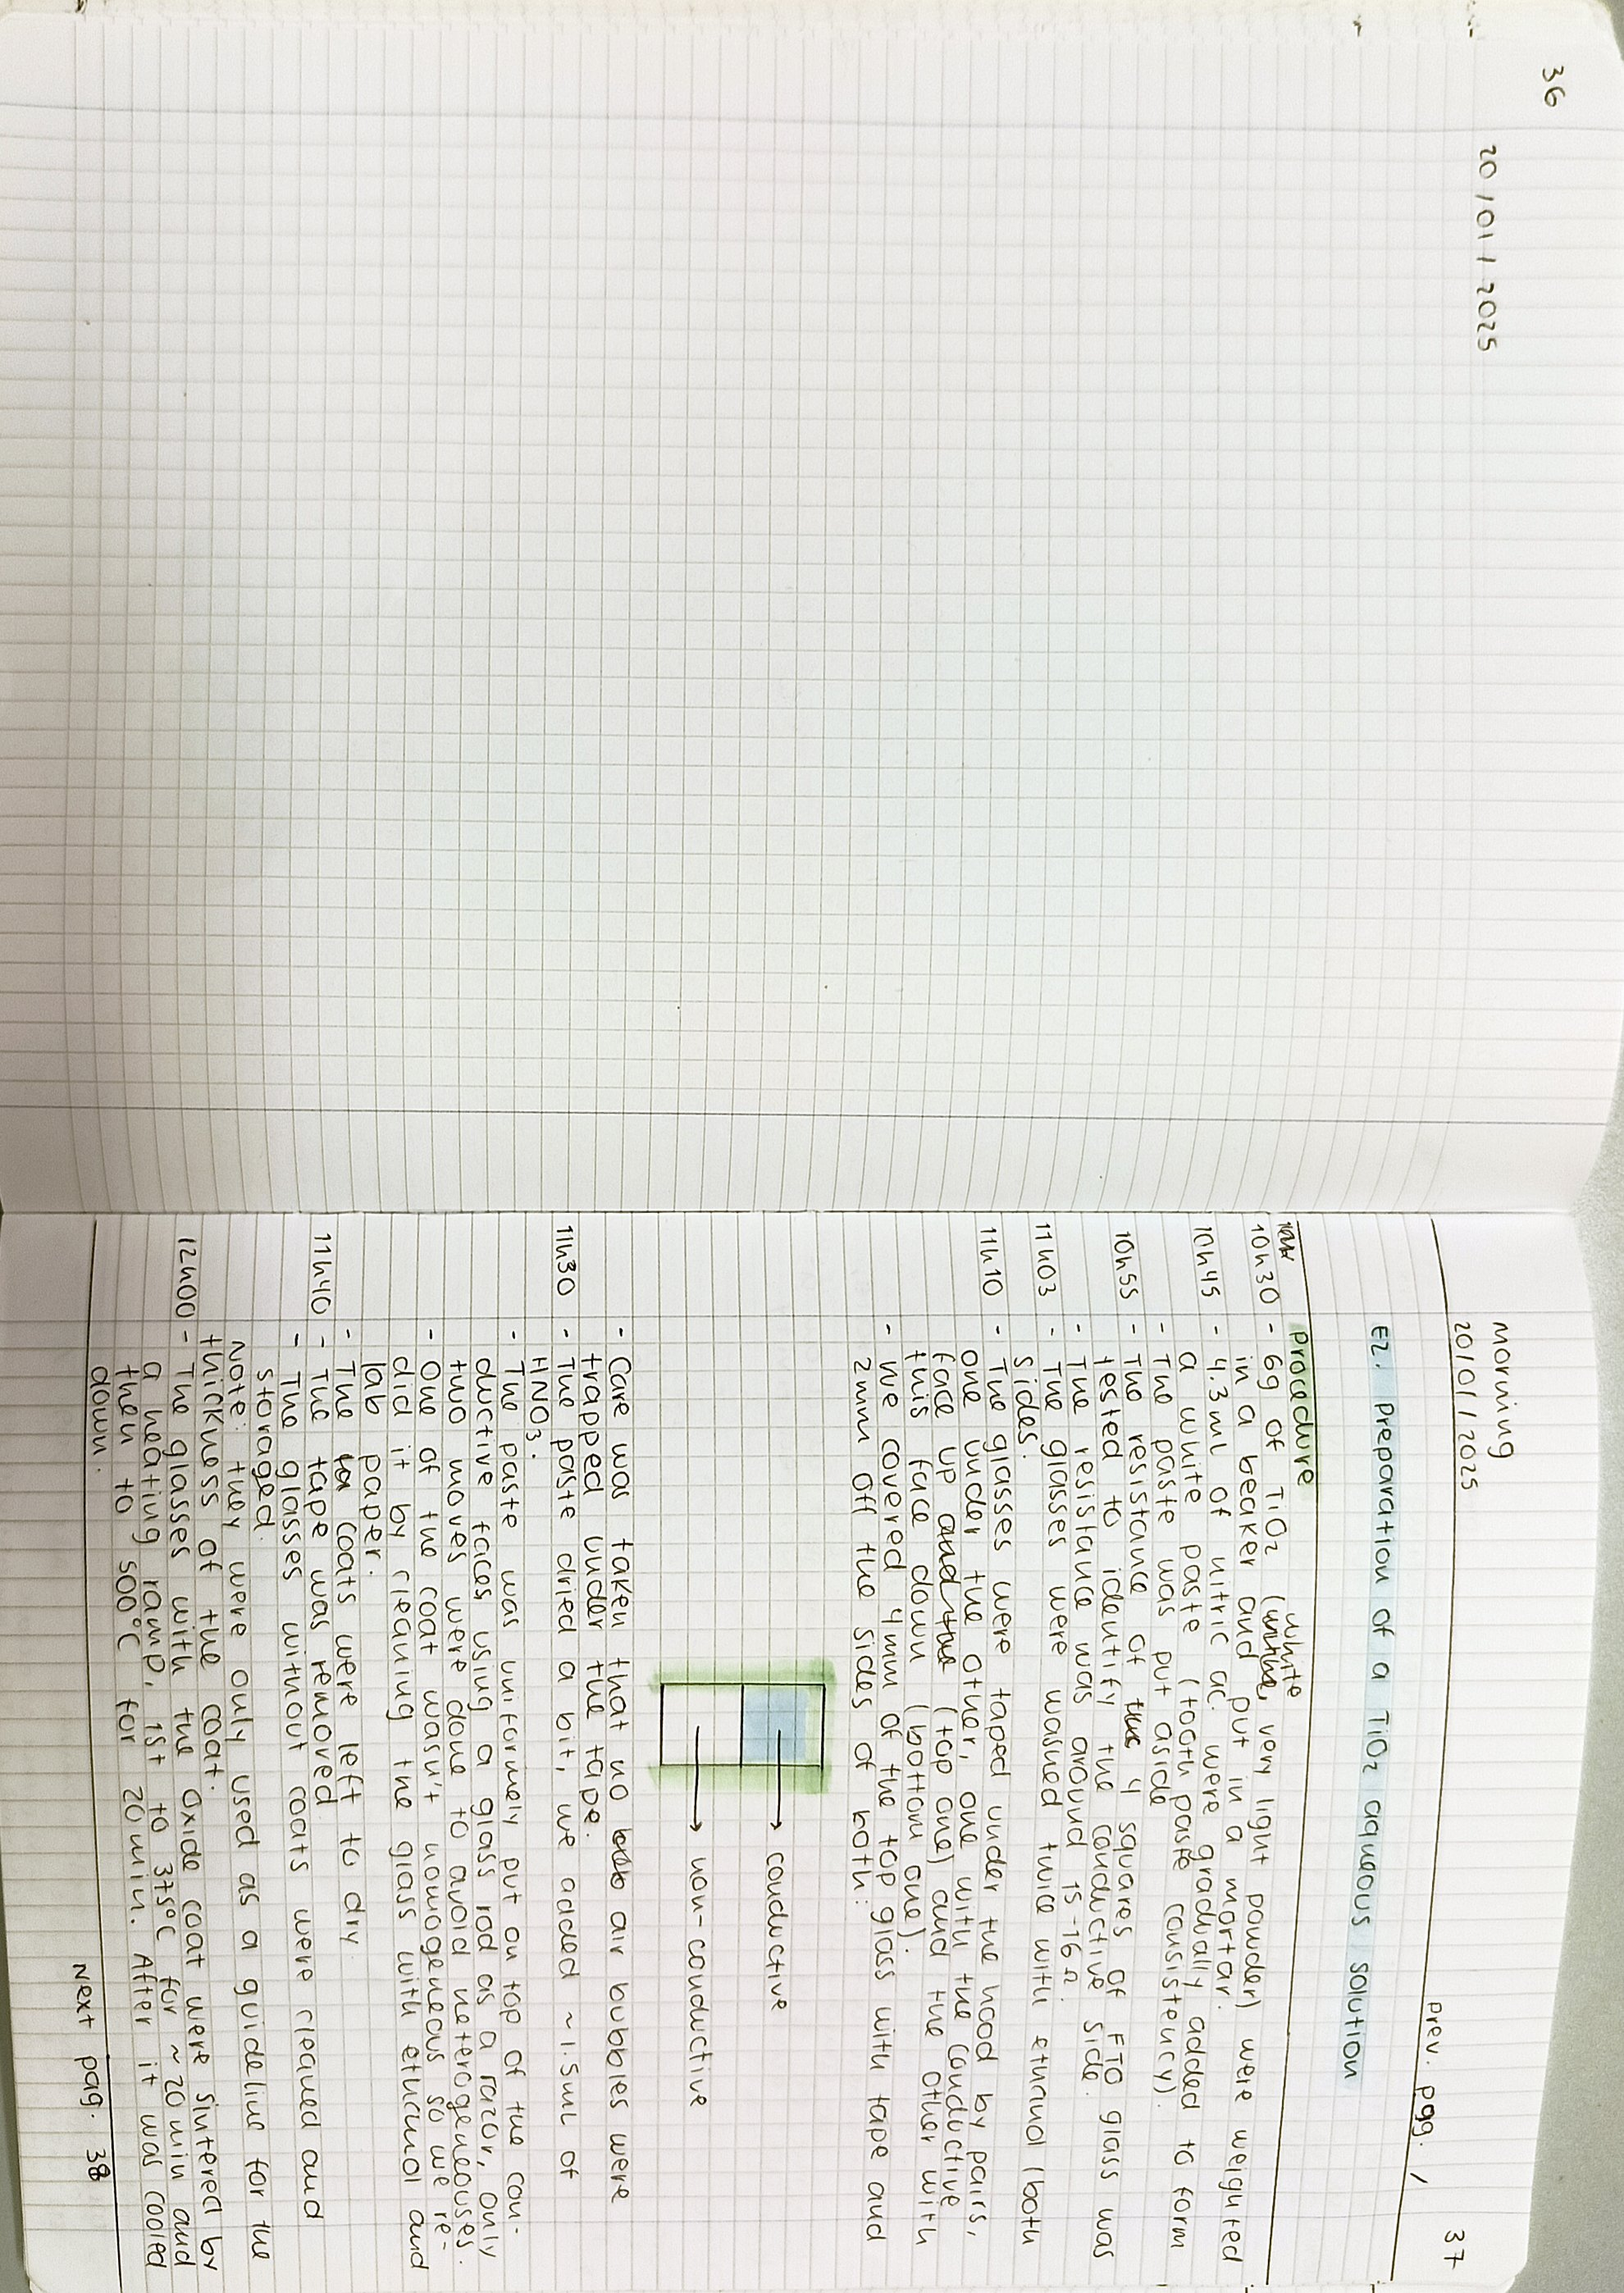
\includegraphics[width=0.6\linewidth, angle=90]{../images/compressed/IMG20250123173058.jpg}
\end{figure}
\begin{figure}[H]
	\centering
	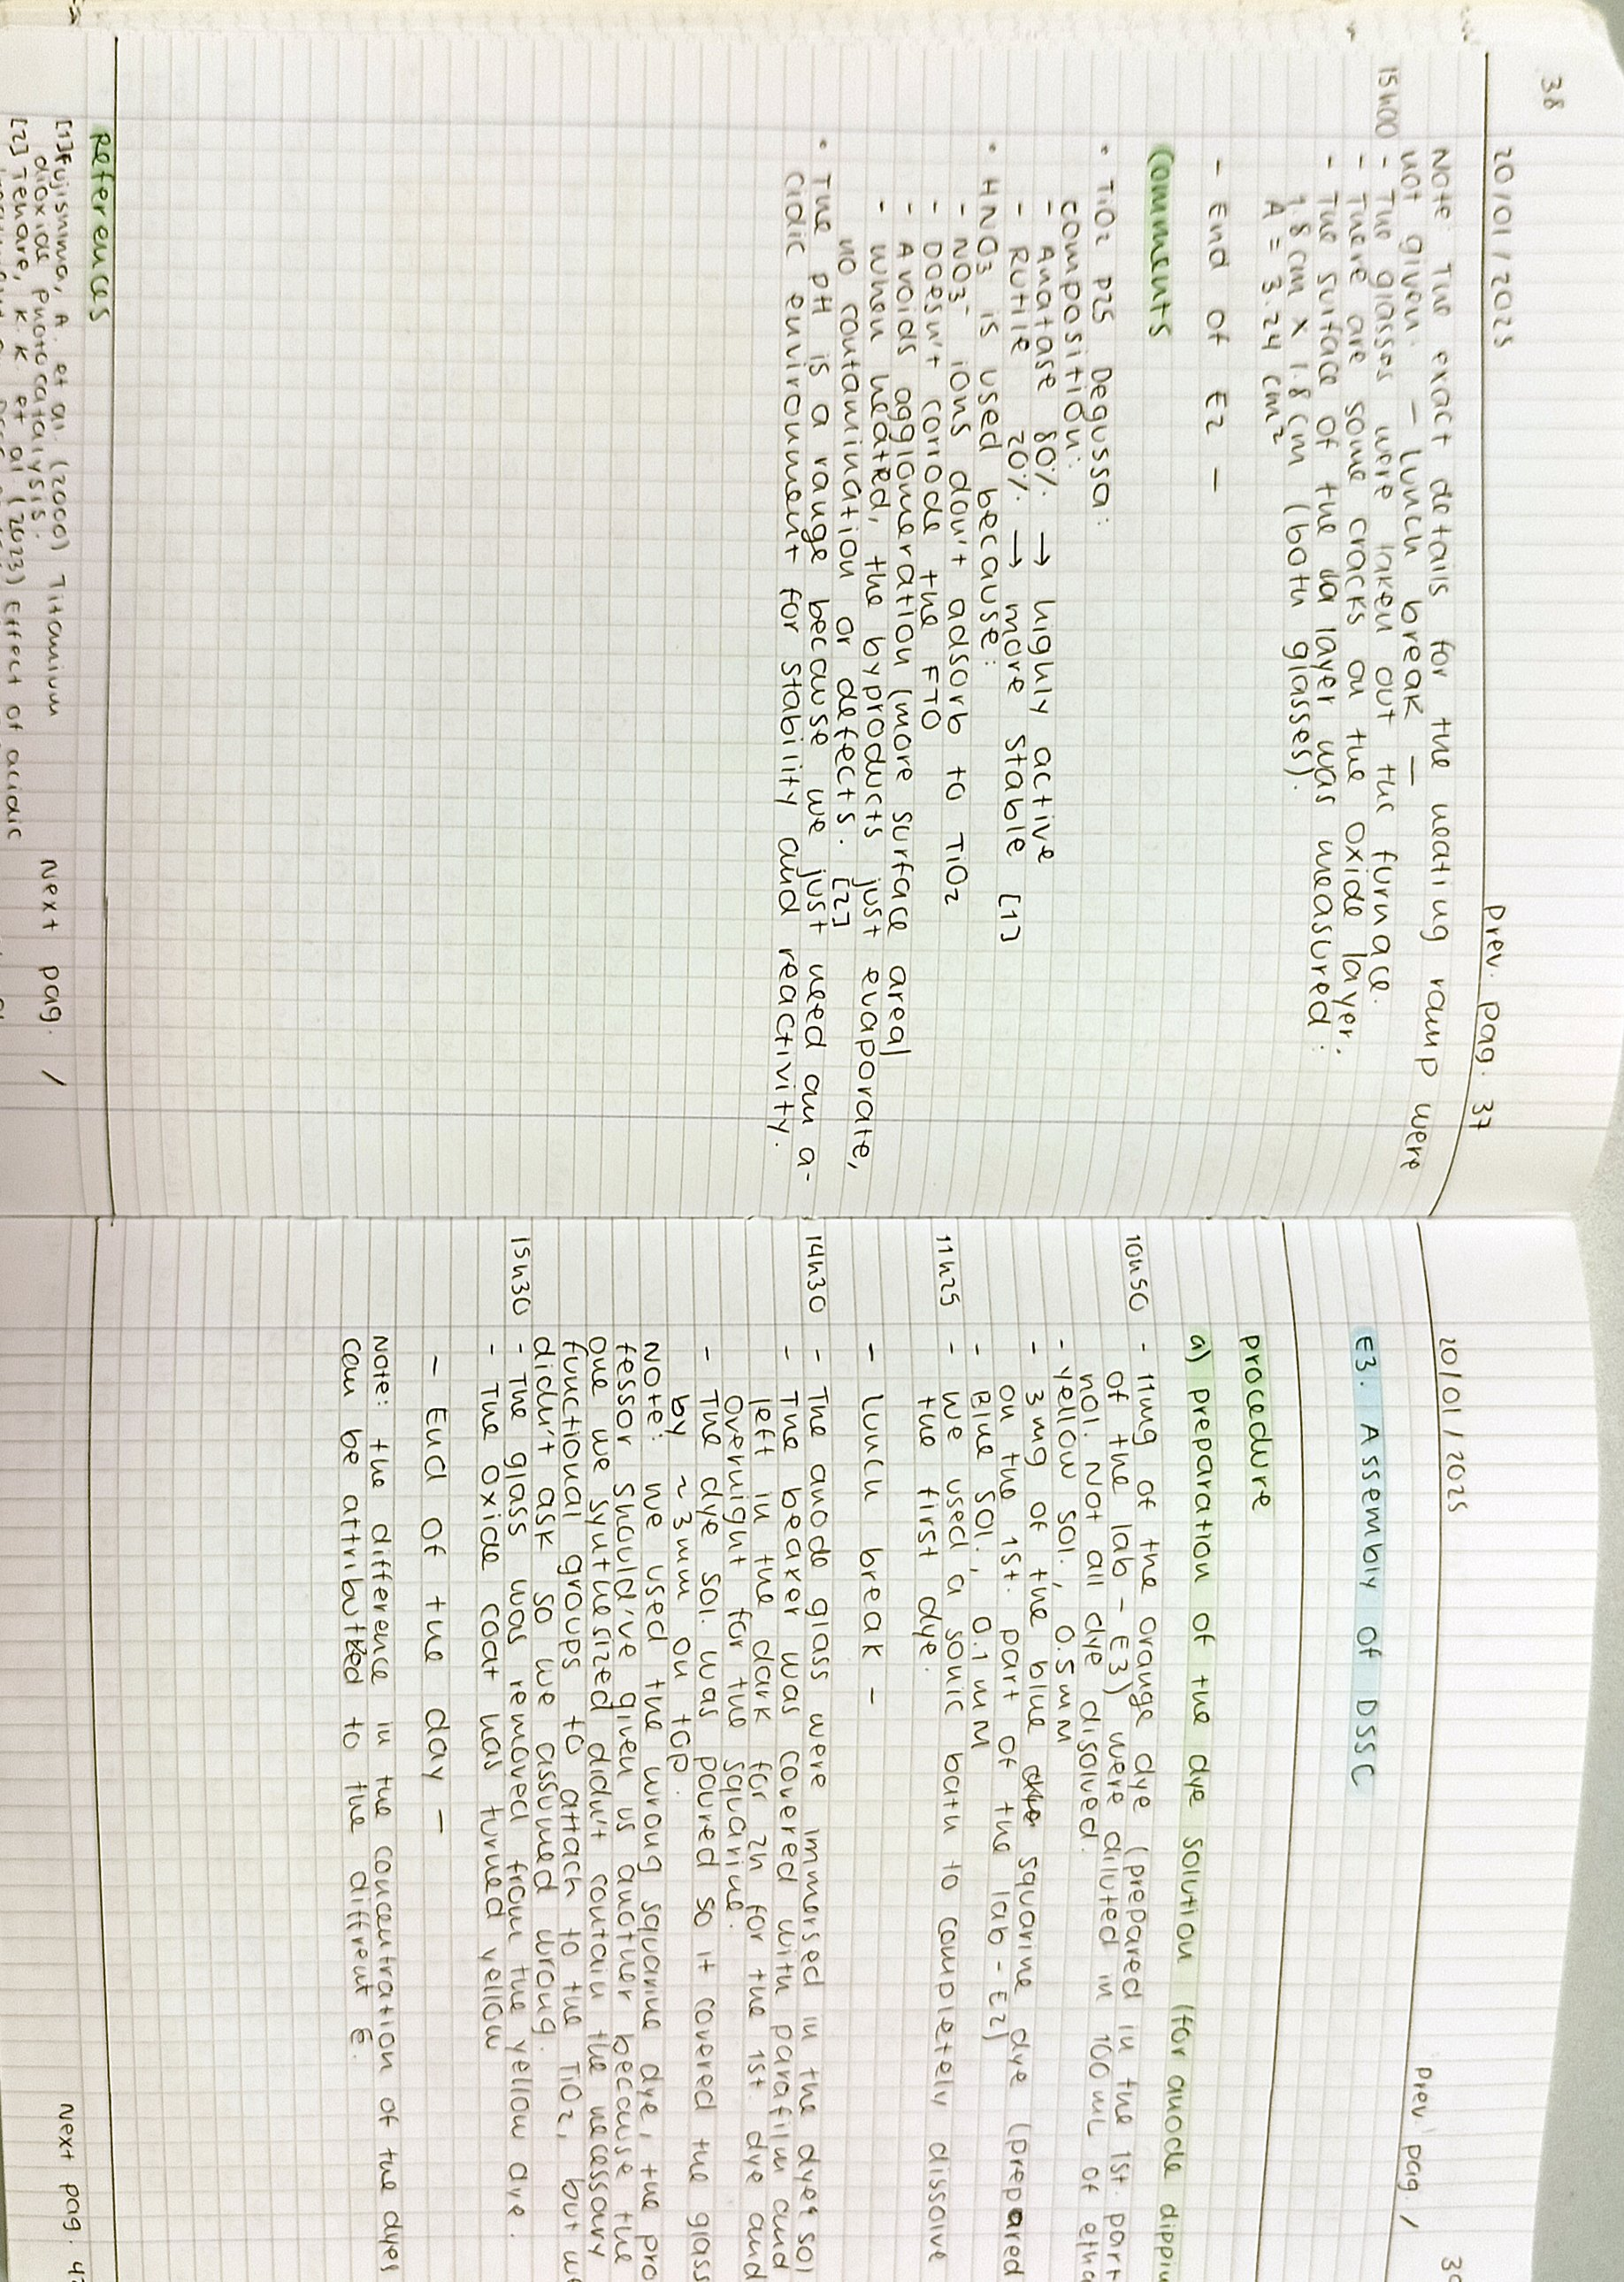
\includegraphics[width=0.6\linewidth, angle=90]{../images/compressed/IMG20250123173103.jpg}
\end{figure}
\begin{figure}[H]
	\centering
	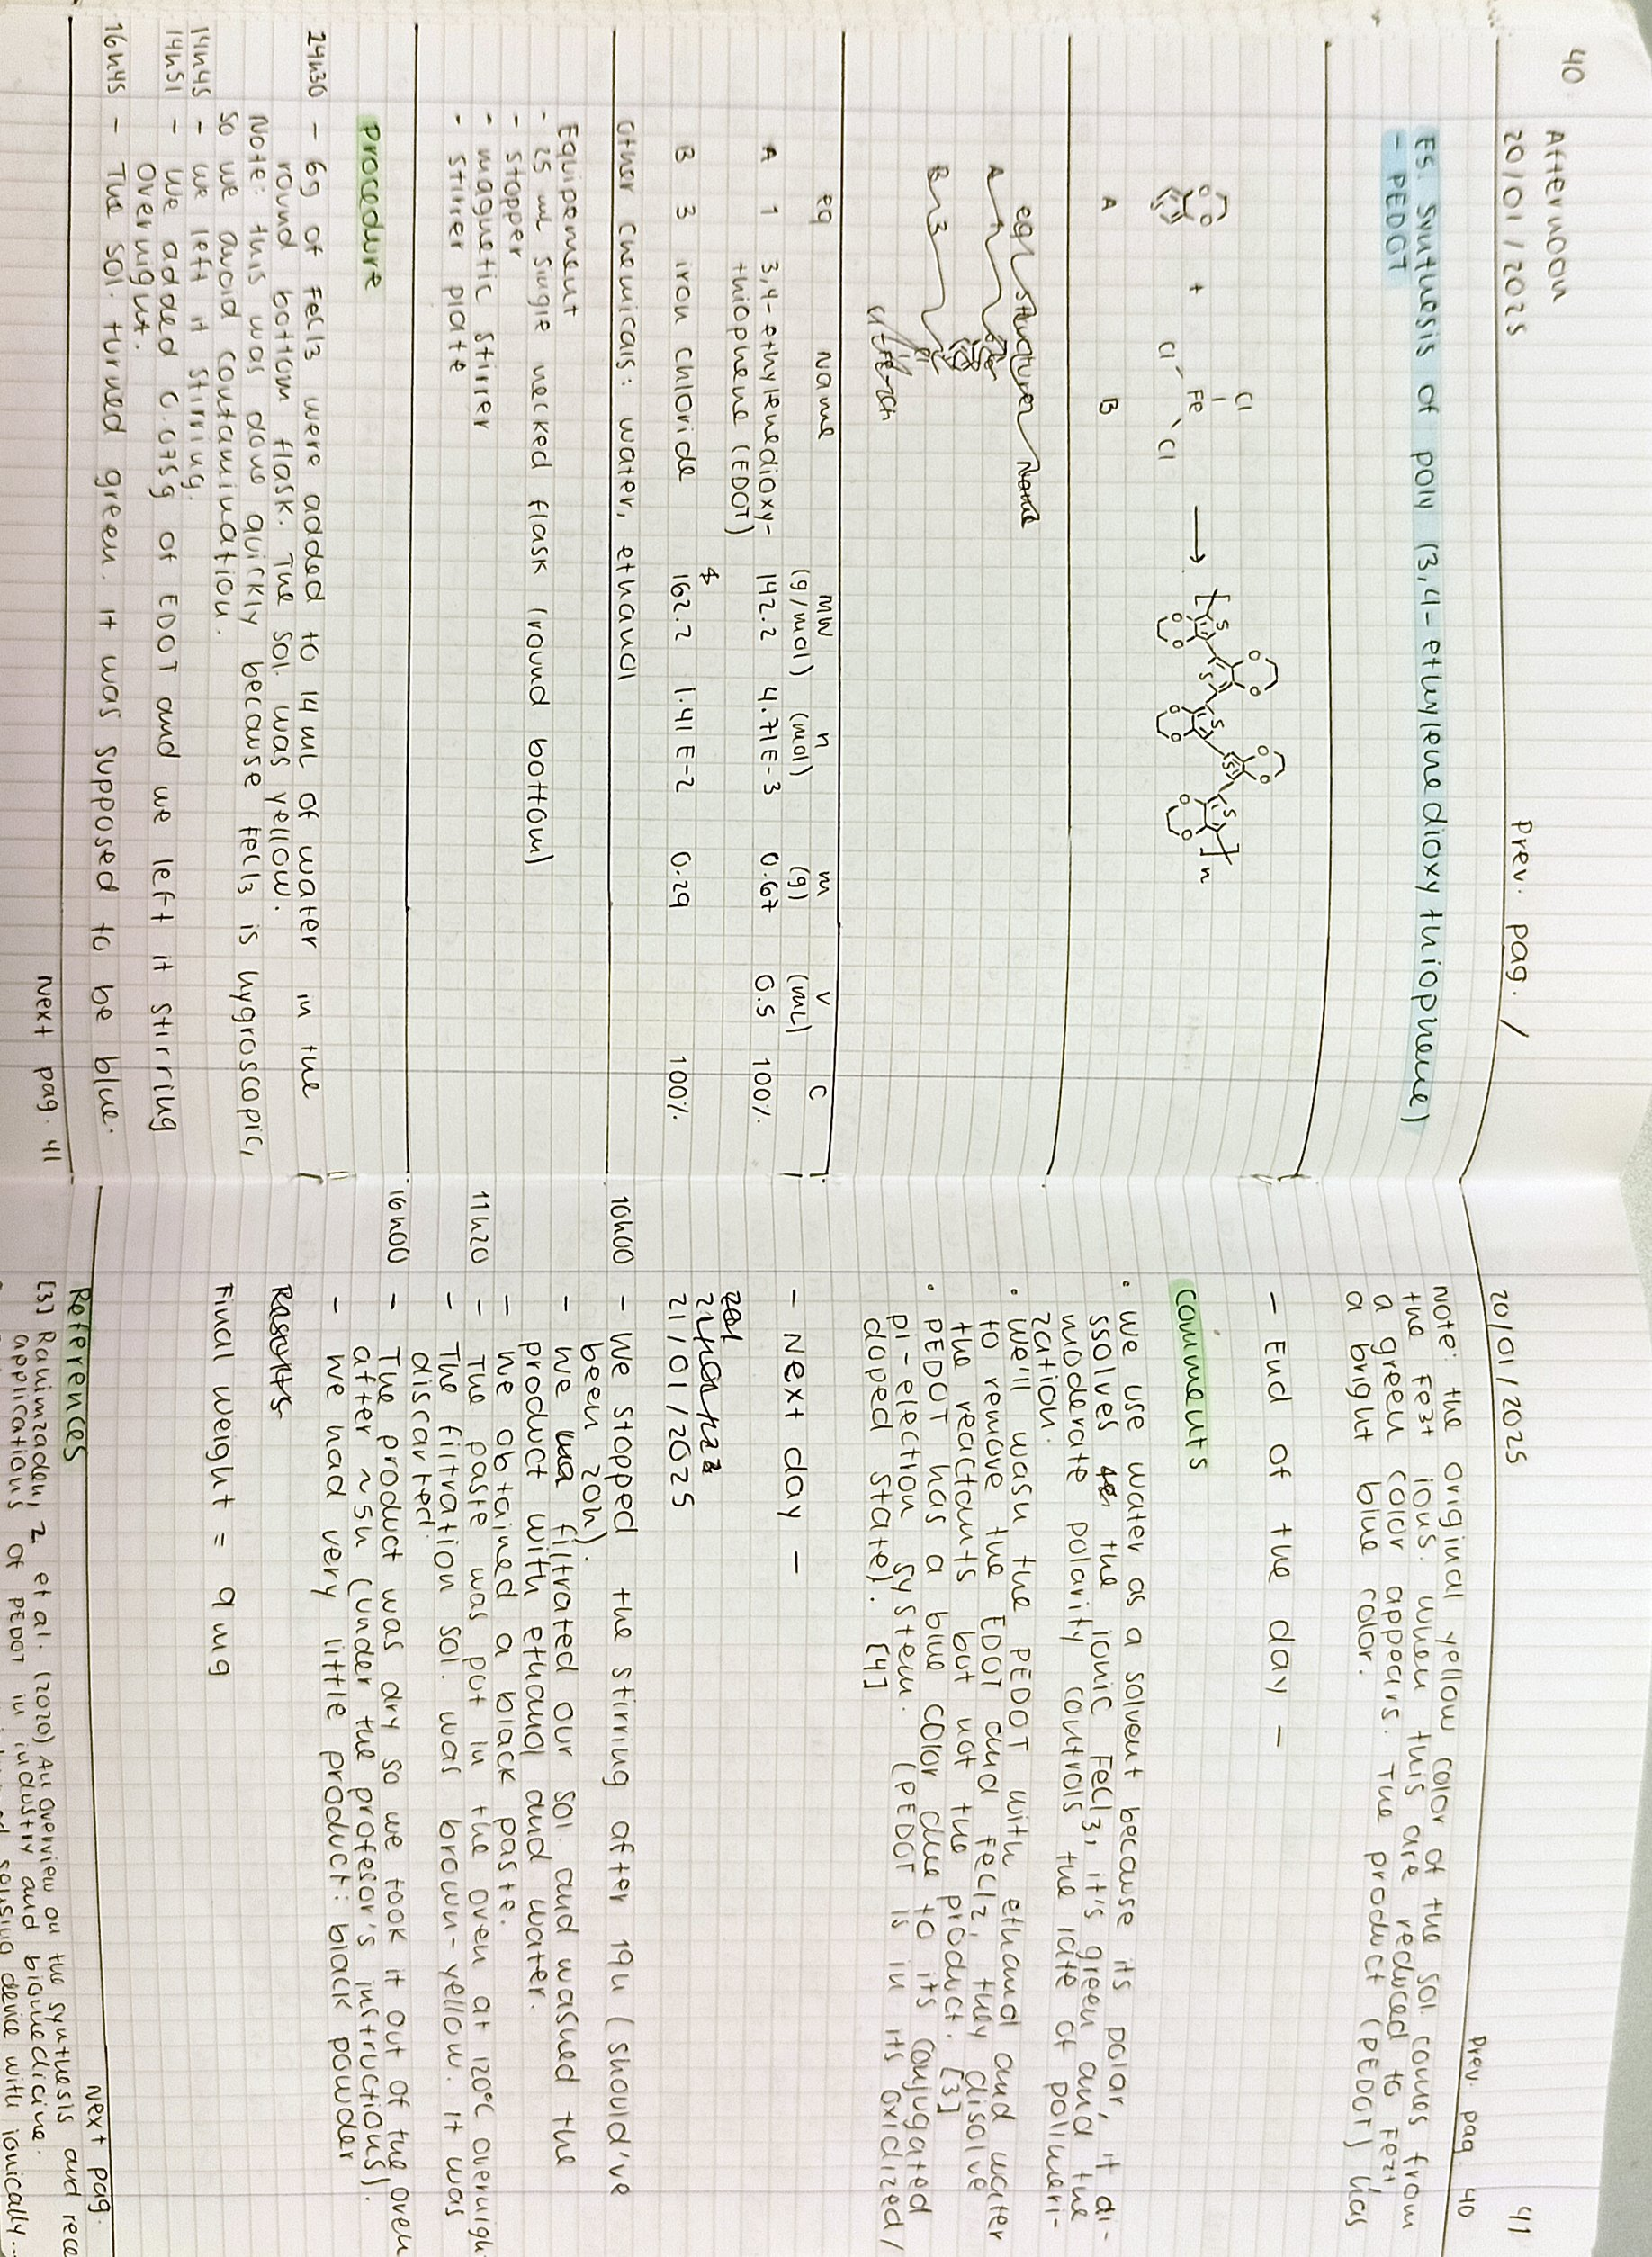
\includegraphics[width=0.6\linewidth, angle=90]{../images/compressed/IMG20250123173107.jpg}
\end{figure}
\begin{figure}[H]
	\centering
	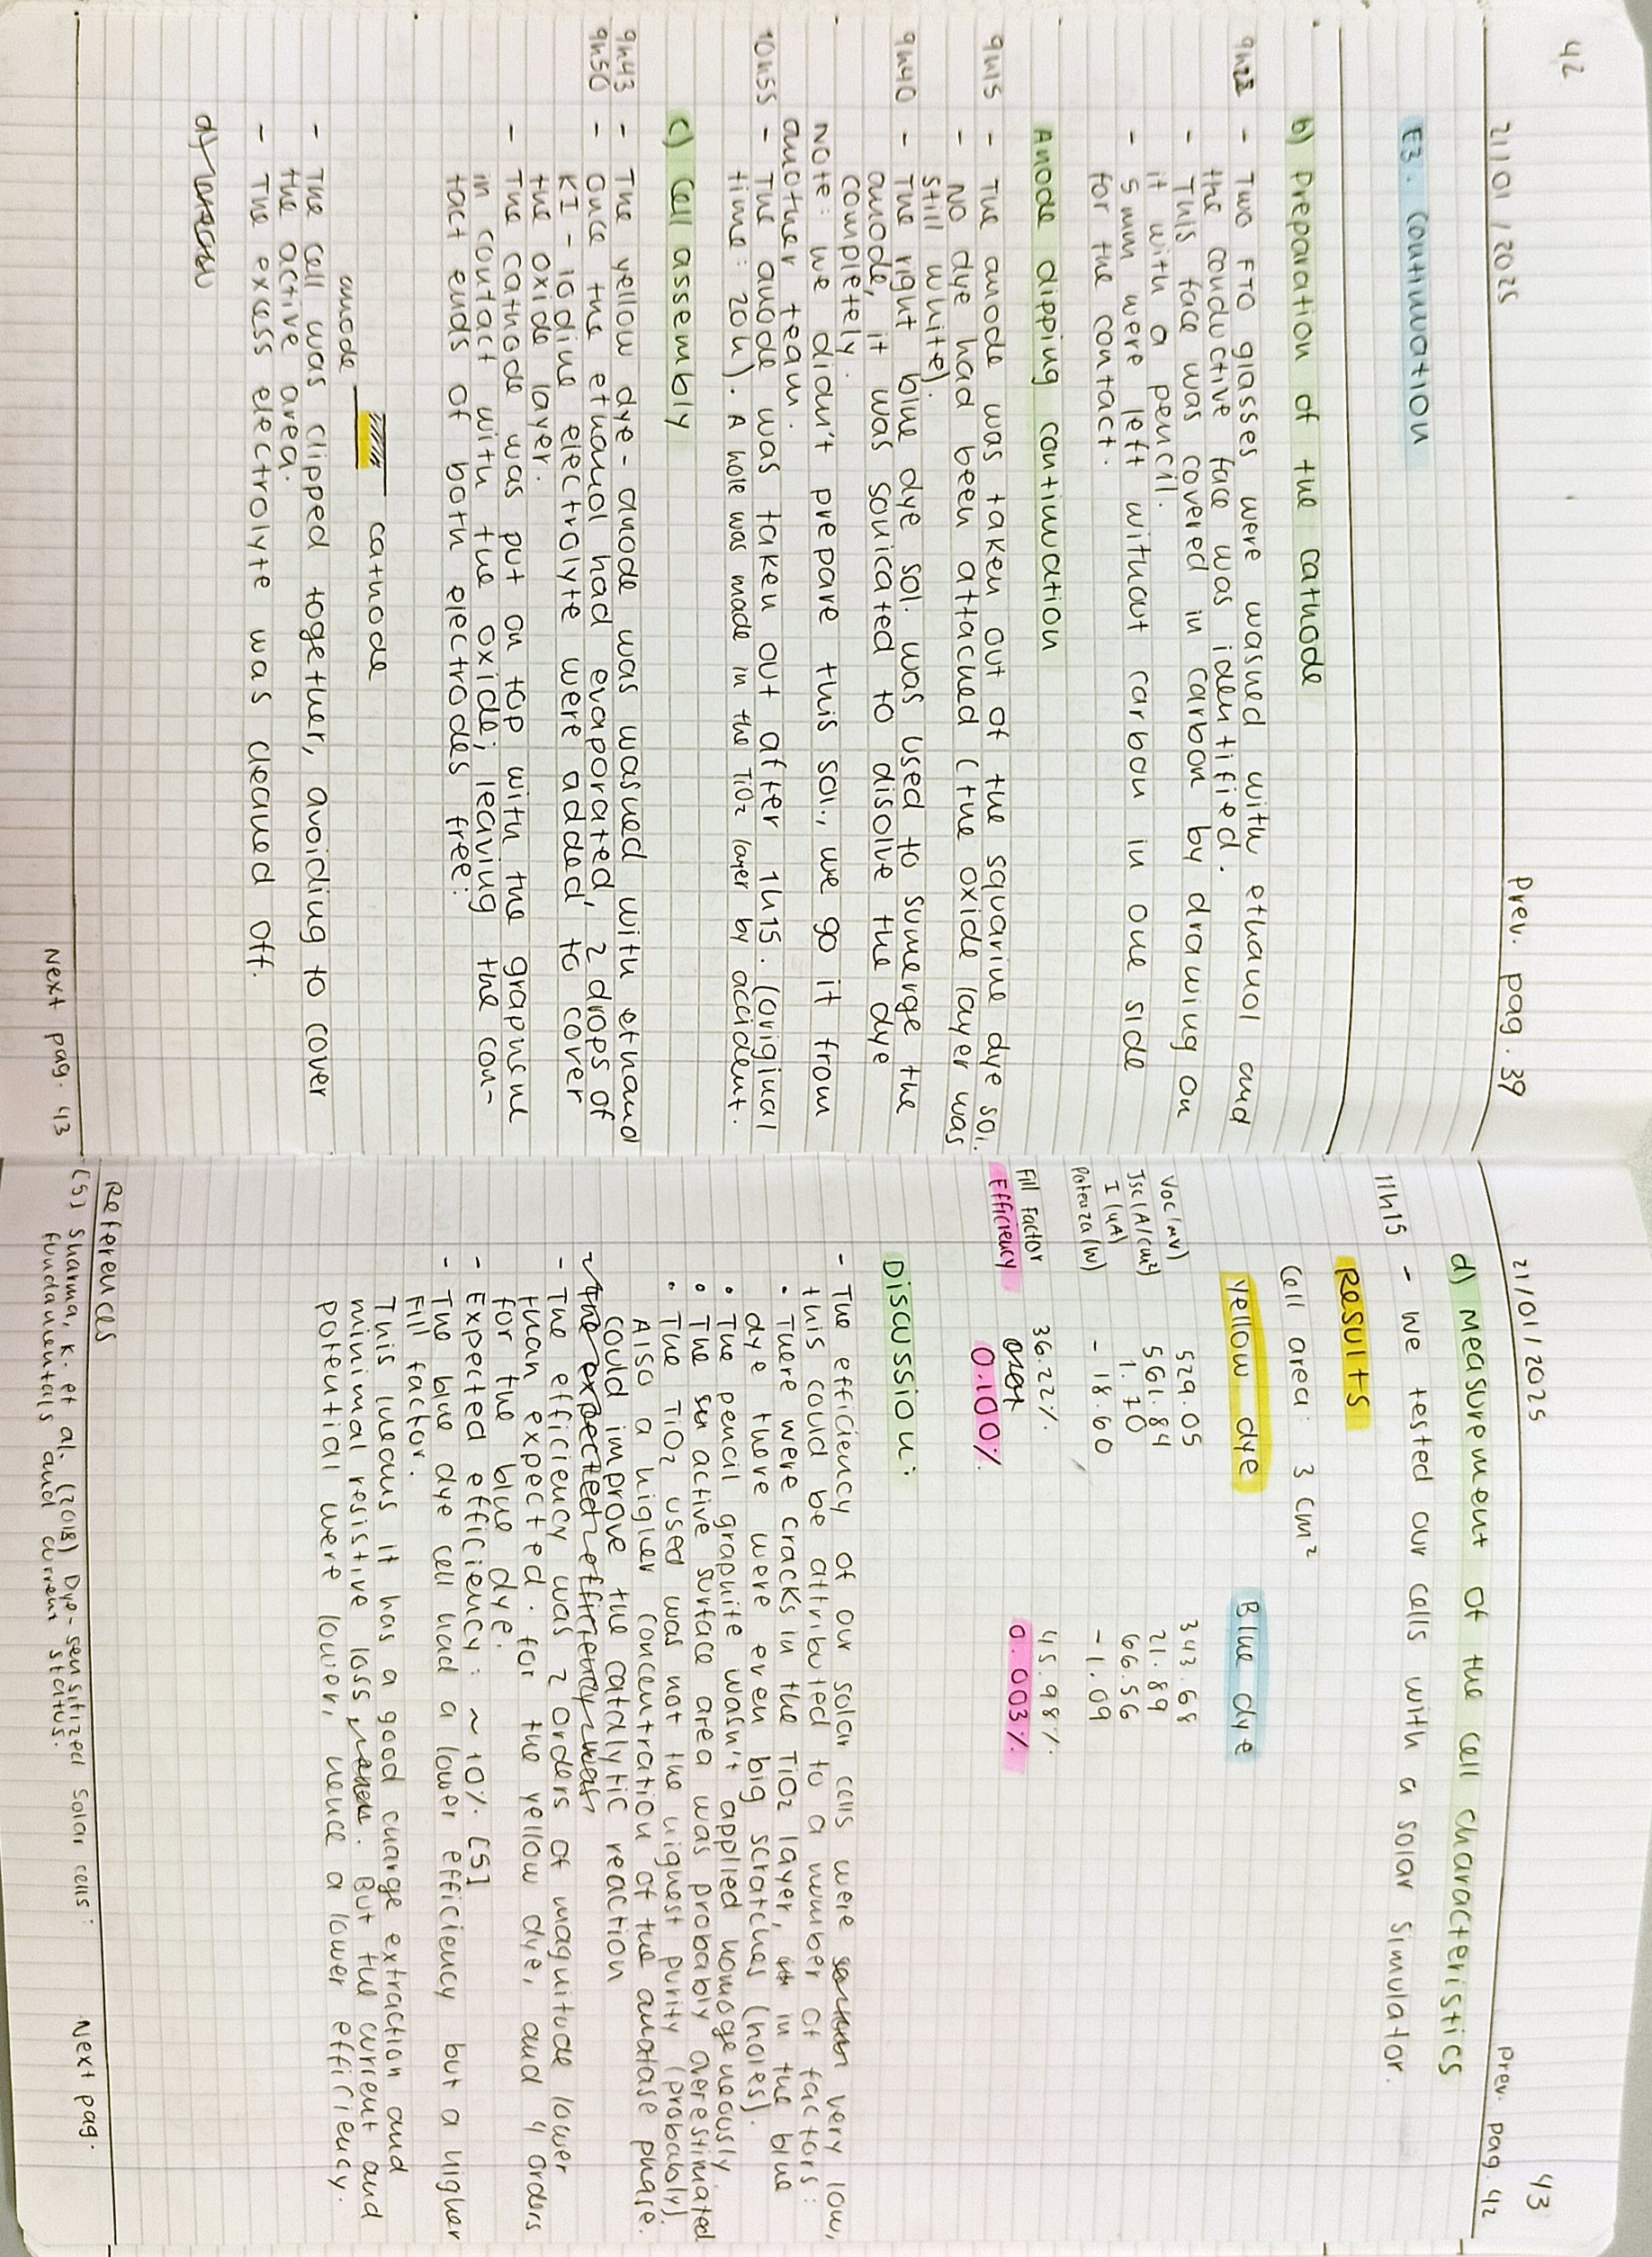
\includegraphics[width=0.6\linewidth, angle=90]{../images/compressed/IMG20250123173112.jpg}
\end{figure}
\begin{figure}[H]
	\centering
	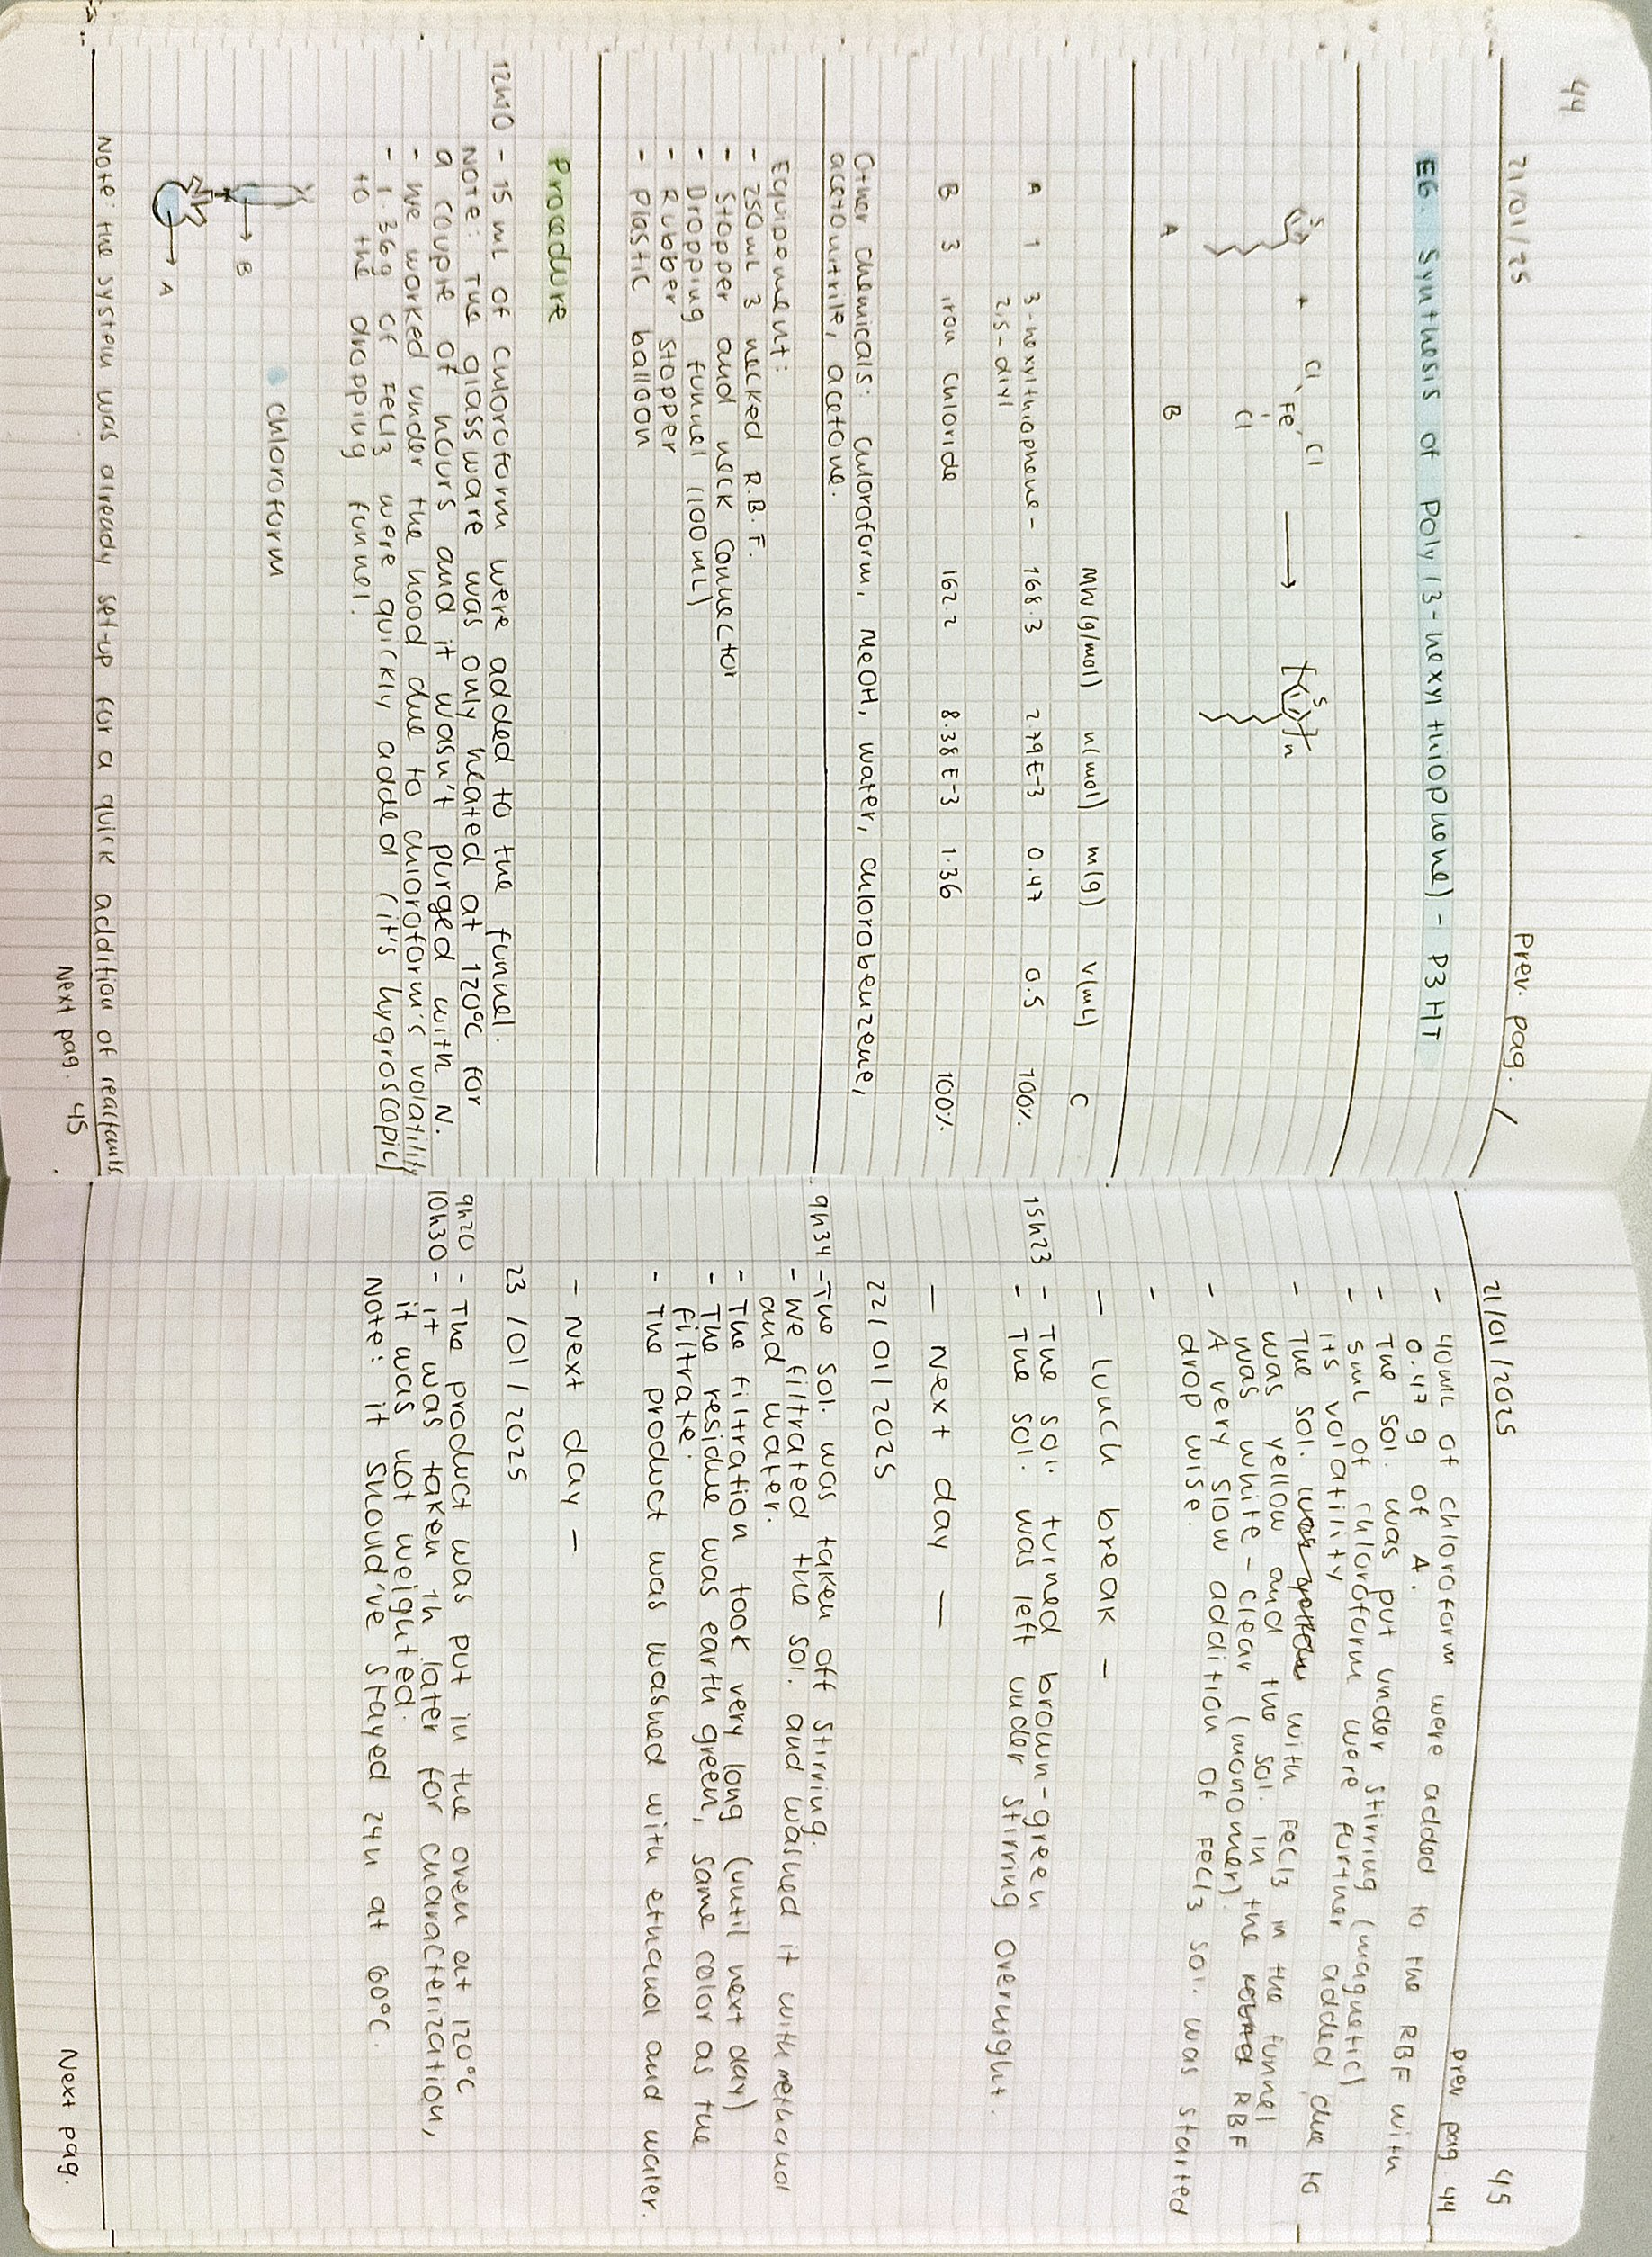
\includegraphics[width=0.6\linewidth, angle=90]{../images/compressed/IMG20250123173118.jpg}
\end{figure}


\subsection{CV curve}
\begin{figure}[H]
	\centering
	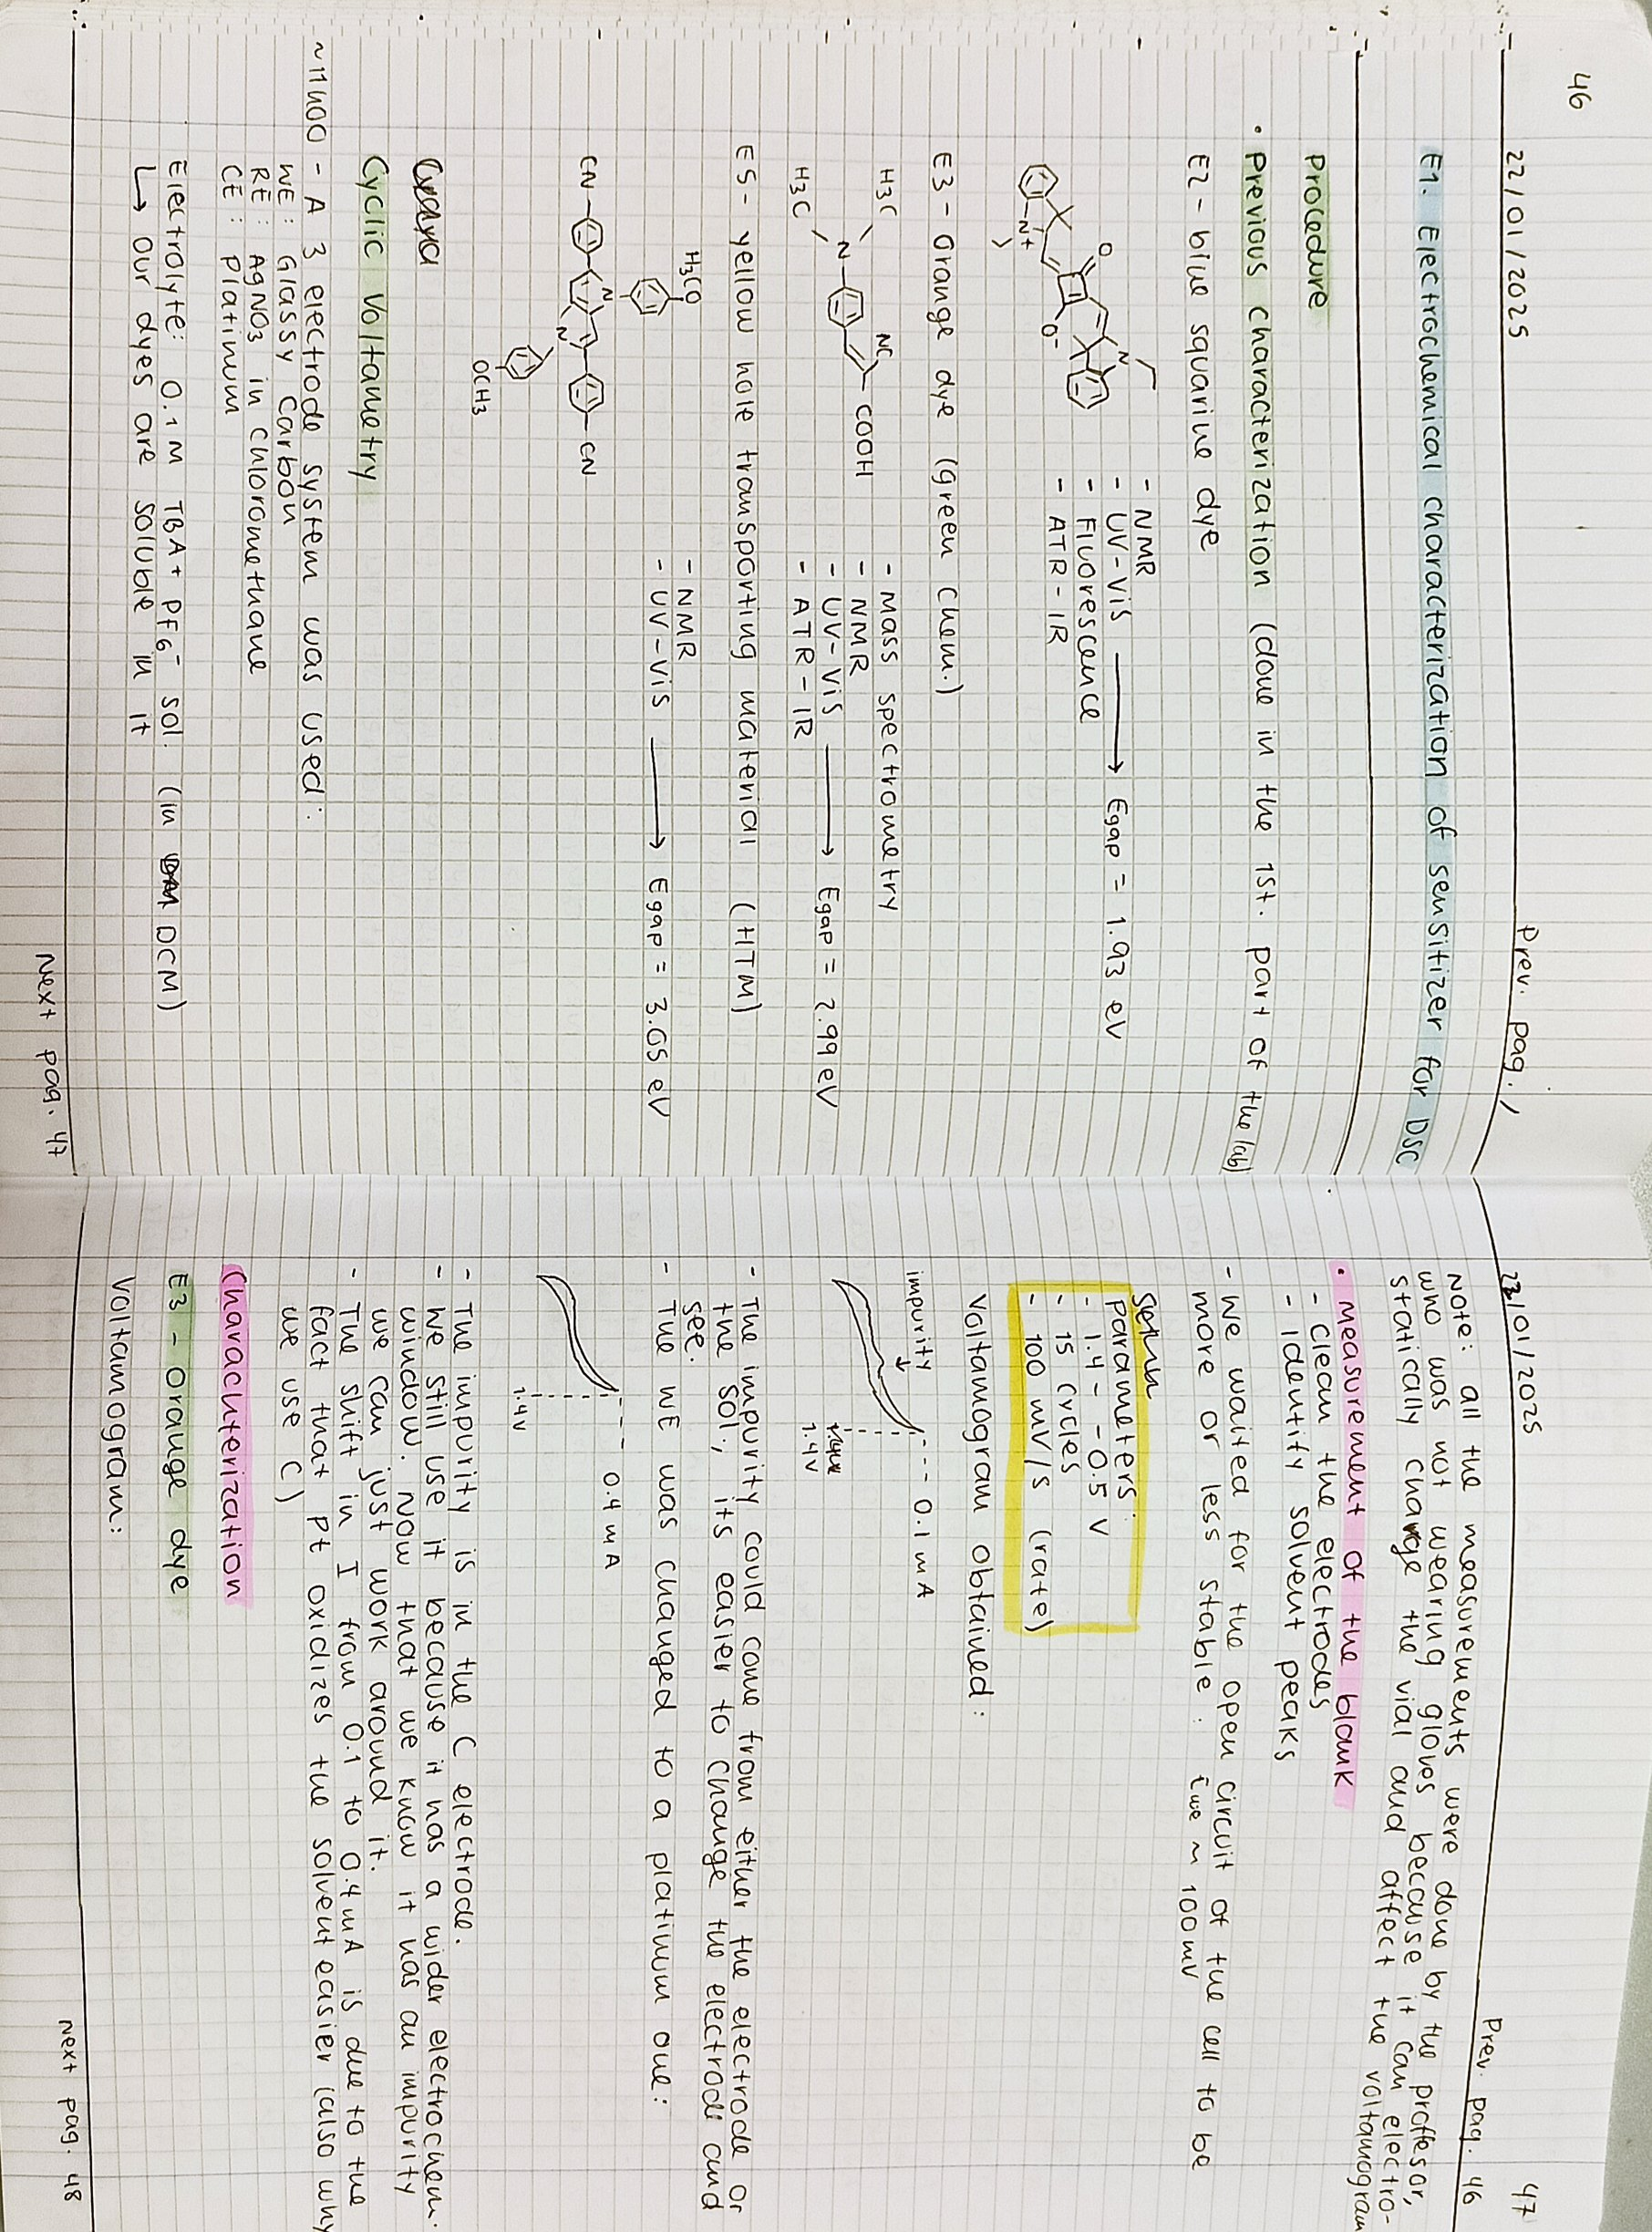
\includegraphics[width=0.6\linewidth, angle=90]{../images/compressed/IMG20250123173124.jpg}
\end{figure}
\begin{figure}[H]
	\centering
	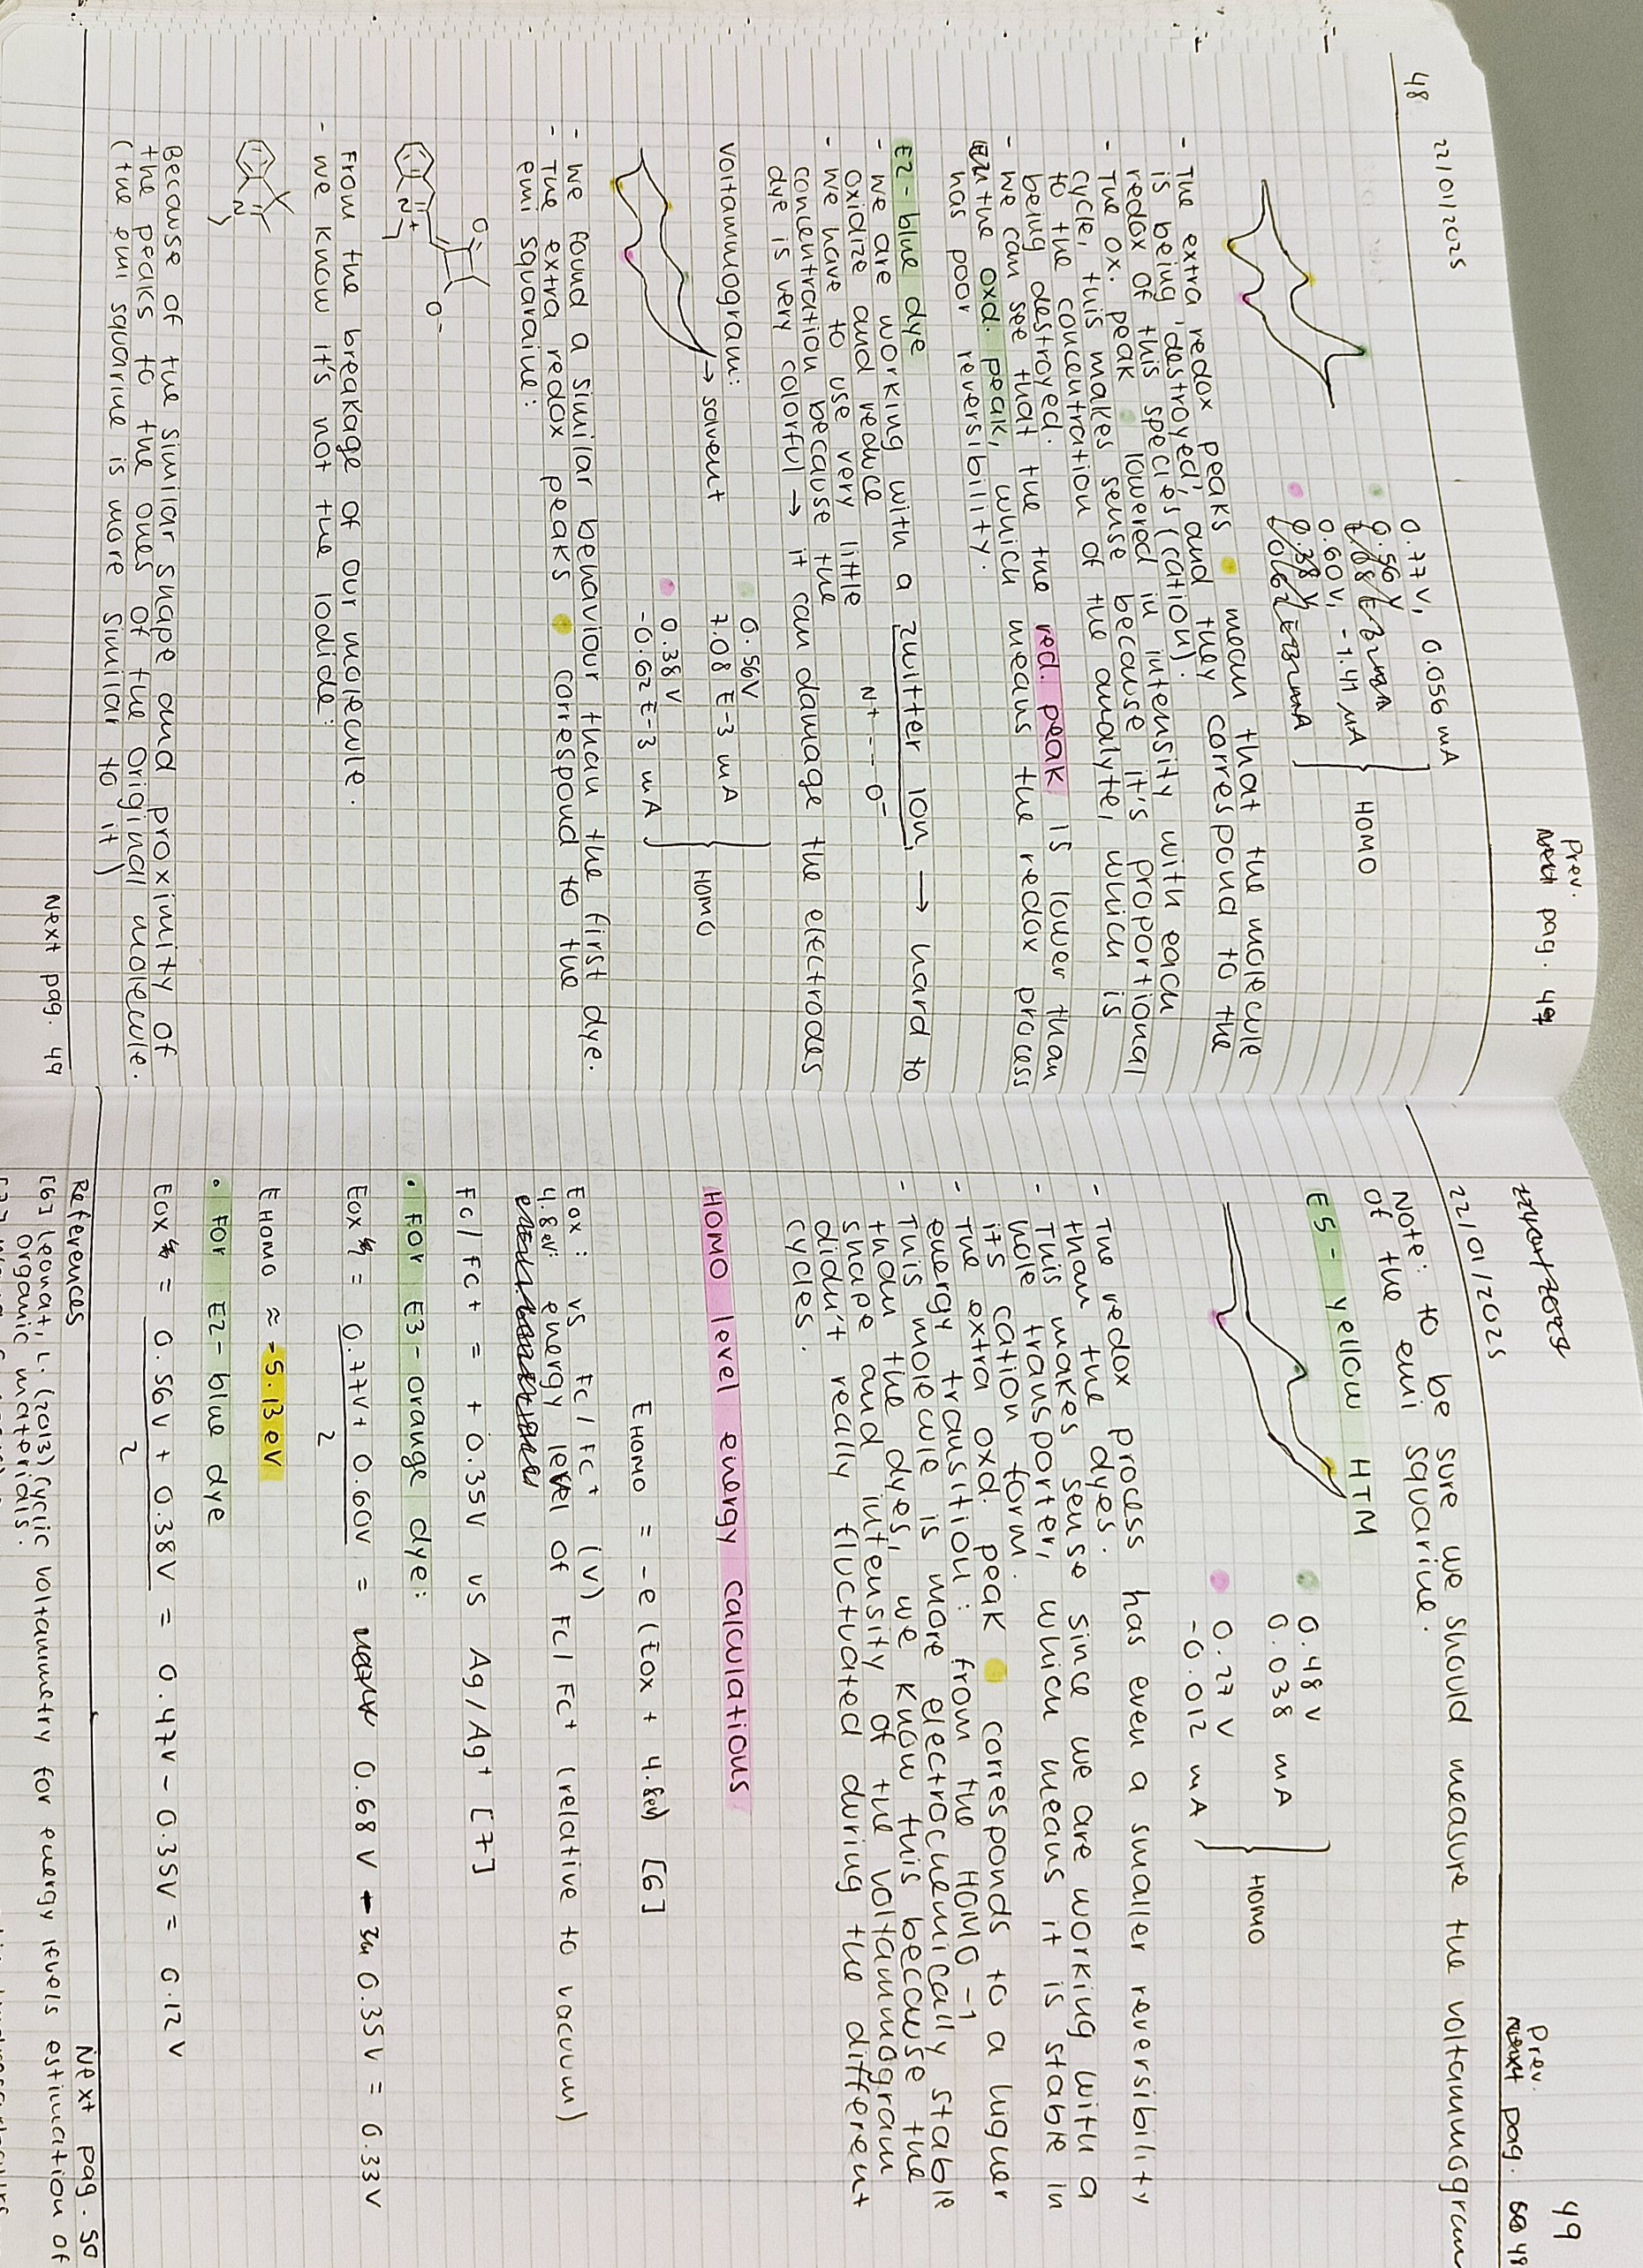
\includegraphics[width=0.6\linewidth, angle=90]{../images/compressed/IMG20250123173131.jpg}
\end{figure}
\begin{figure}[H]
	\centering
	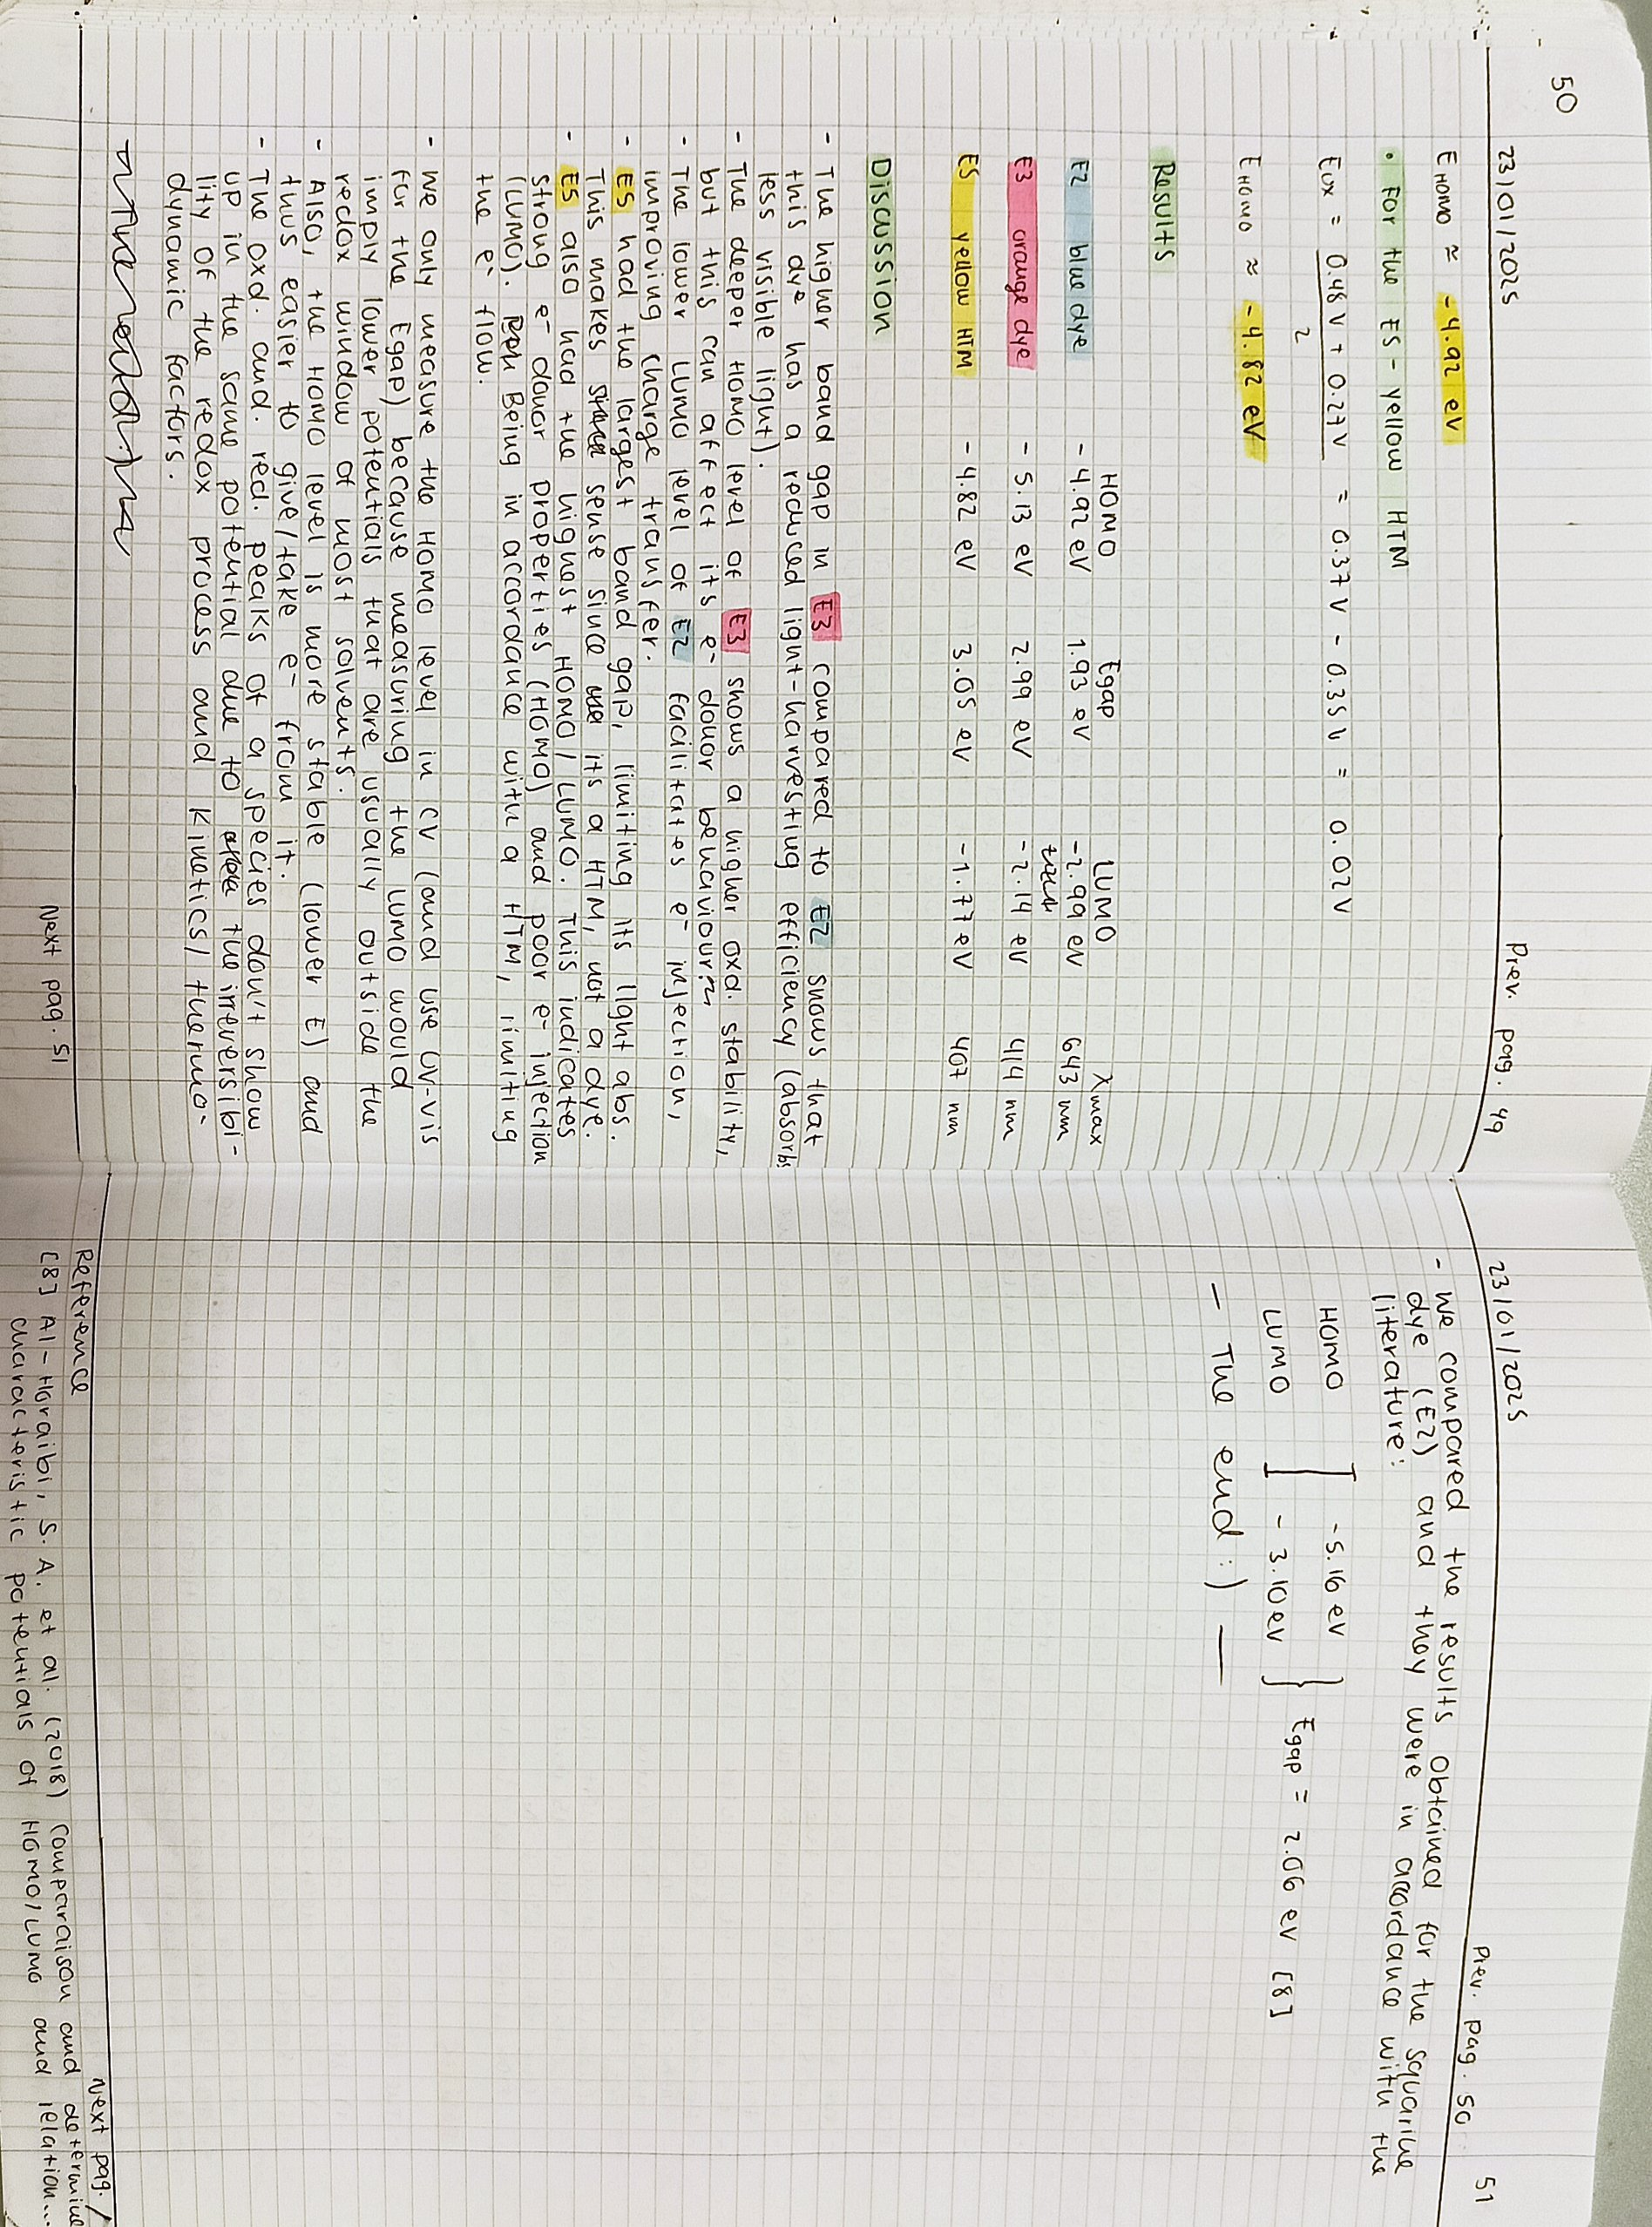
\includegraphics[width=0.6\linewidth, angle=90]{../images/compressed/IMG20250123173139.jpg}
\end{figure}


\subsection{TGA \& DSC}
\begin{figure}[H]
	\centering
	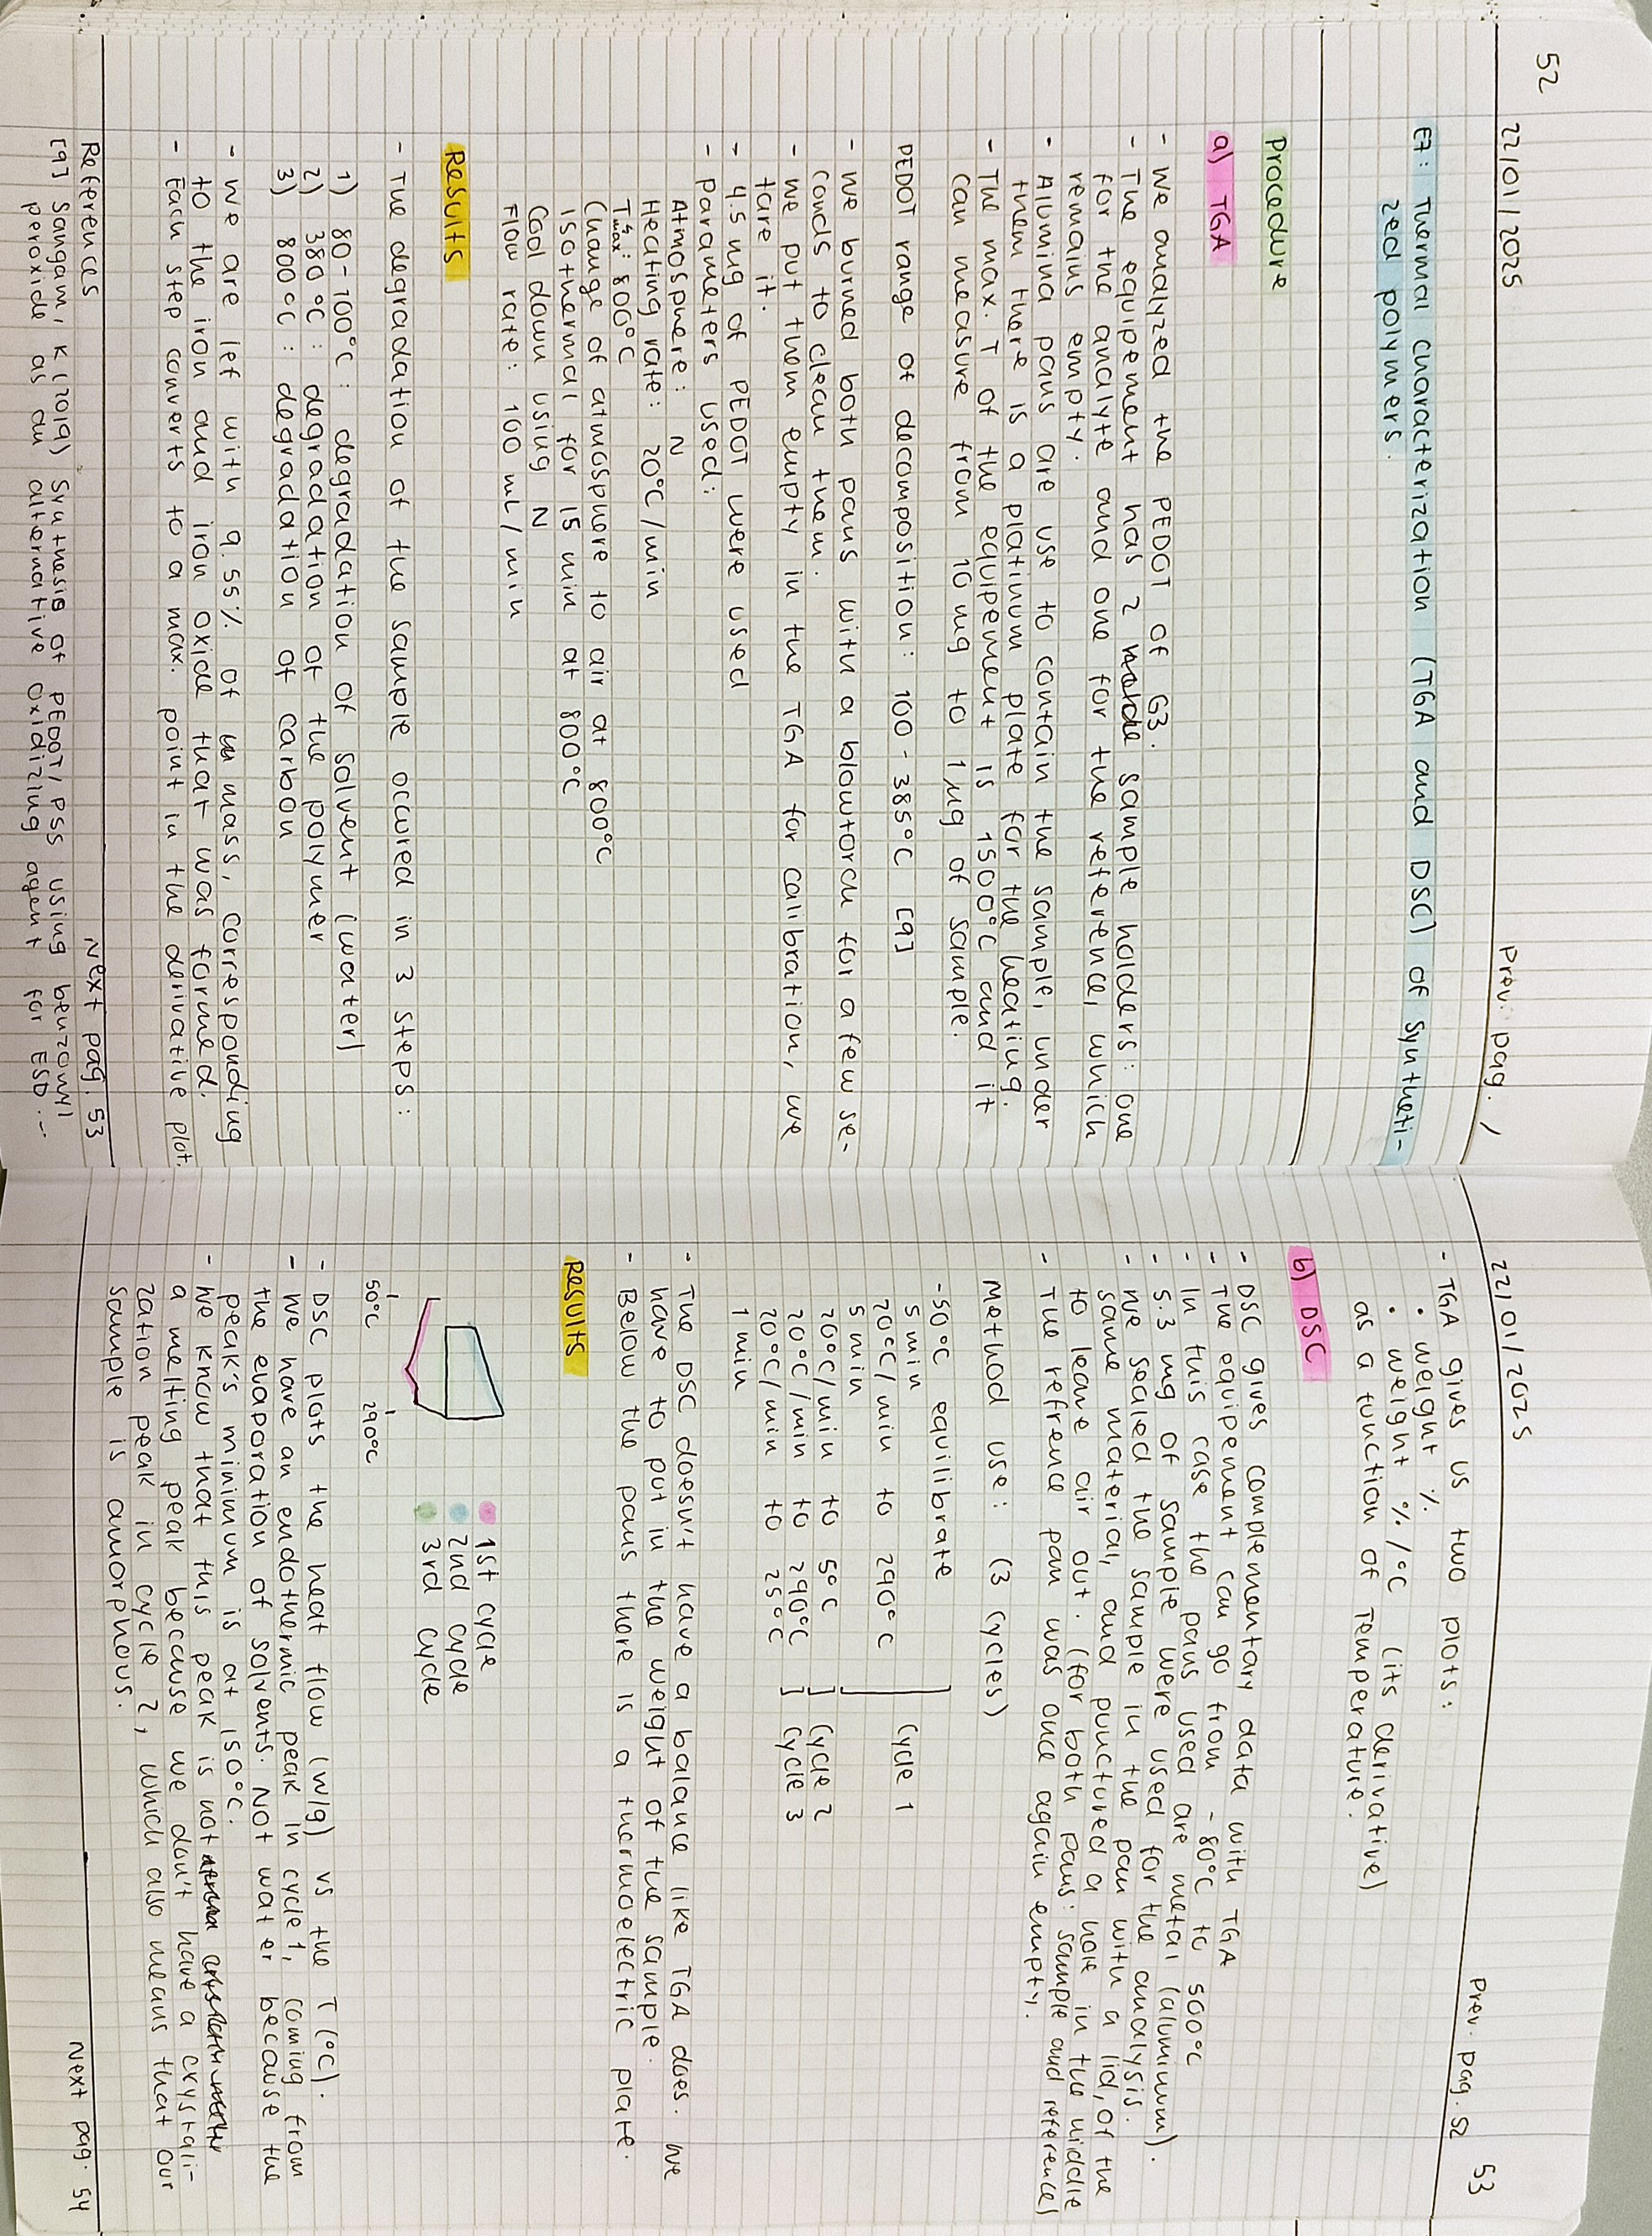
\includegraphics[width=0.6\linewidth, angle=90]{../images/compressed/IMG20250123173147.jpg}
\end{figure}
\begin{figure}[H]
	\centering
	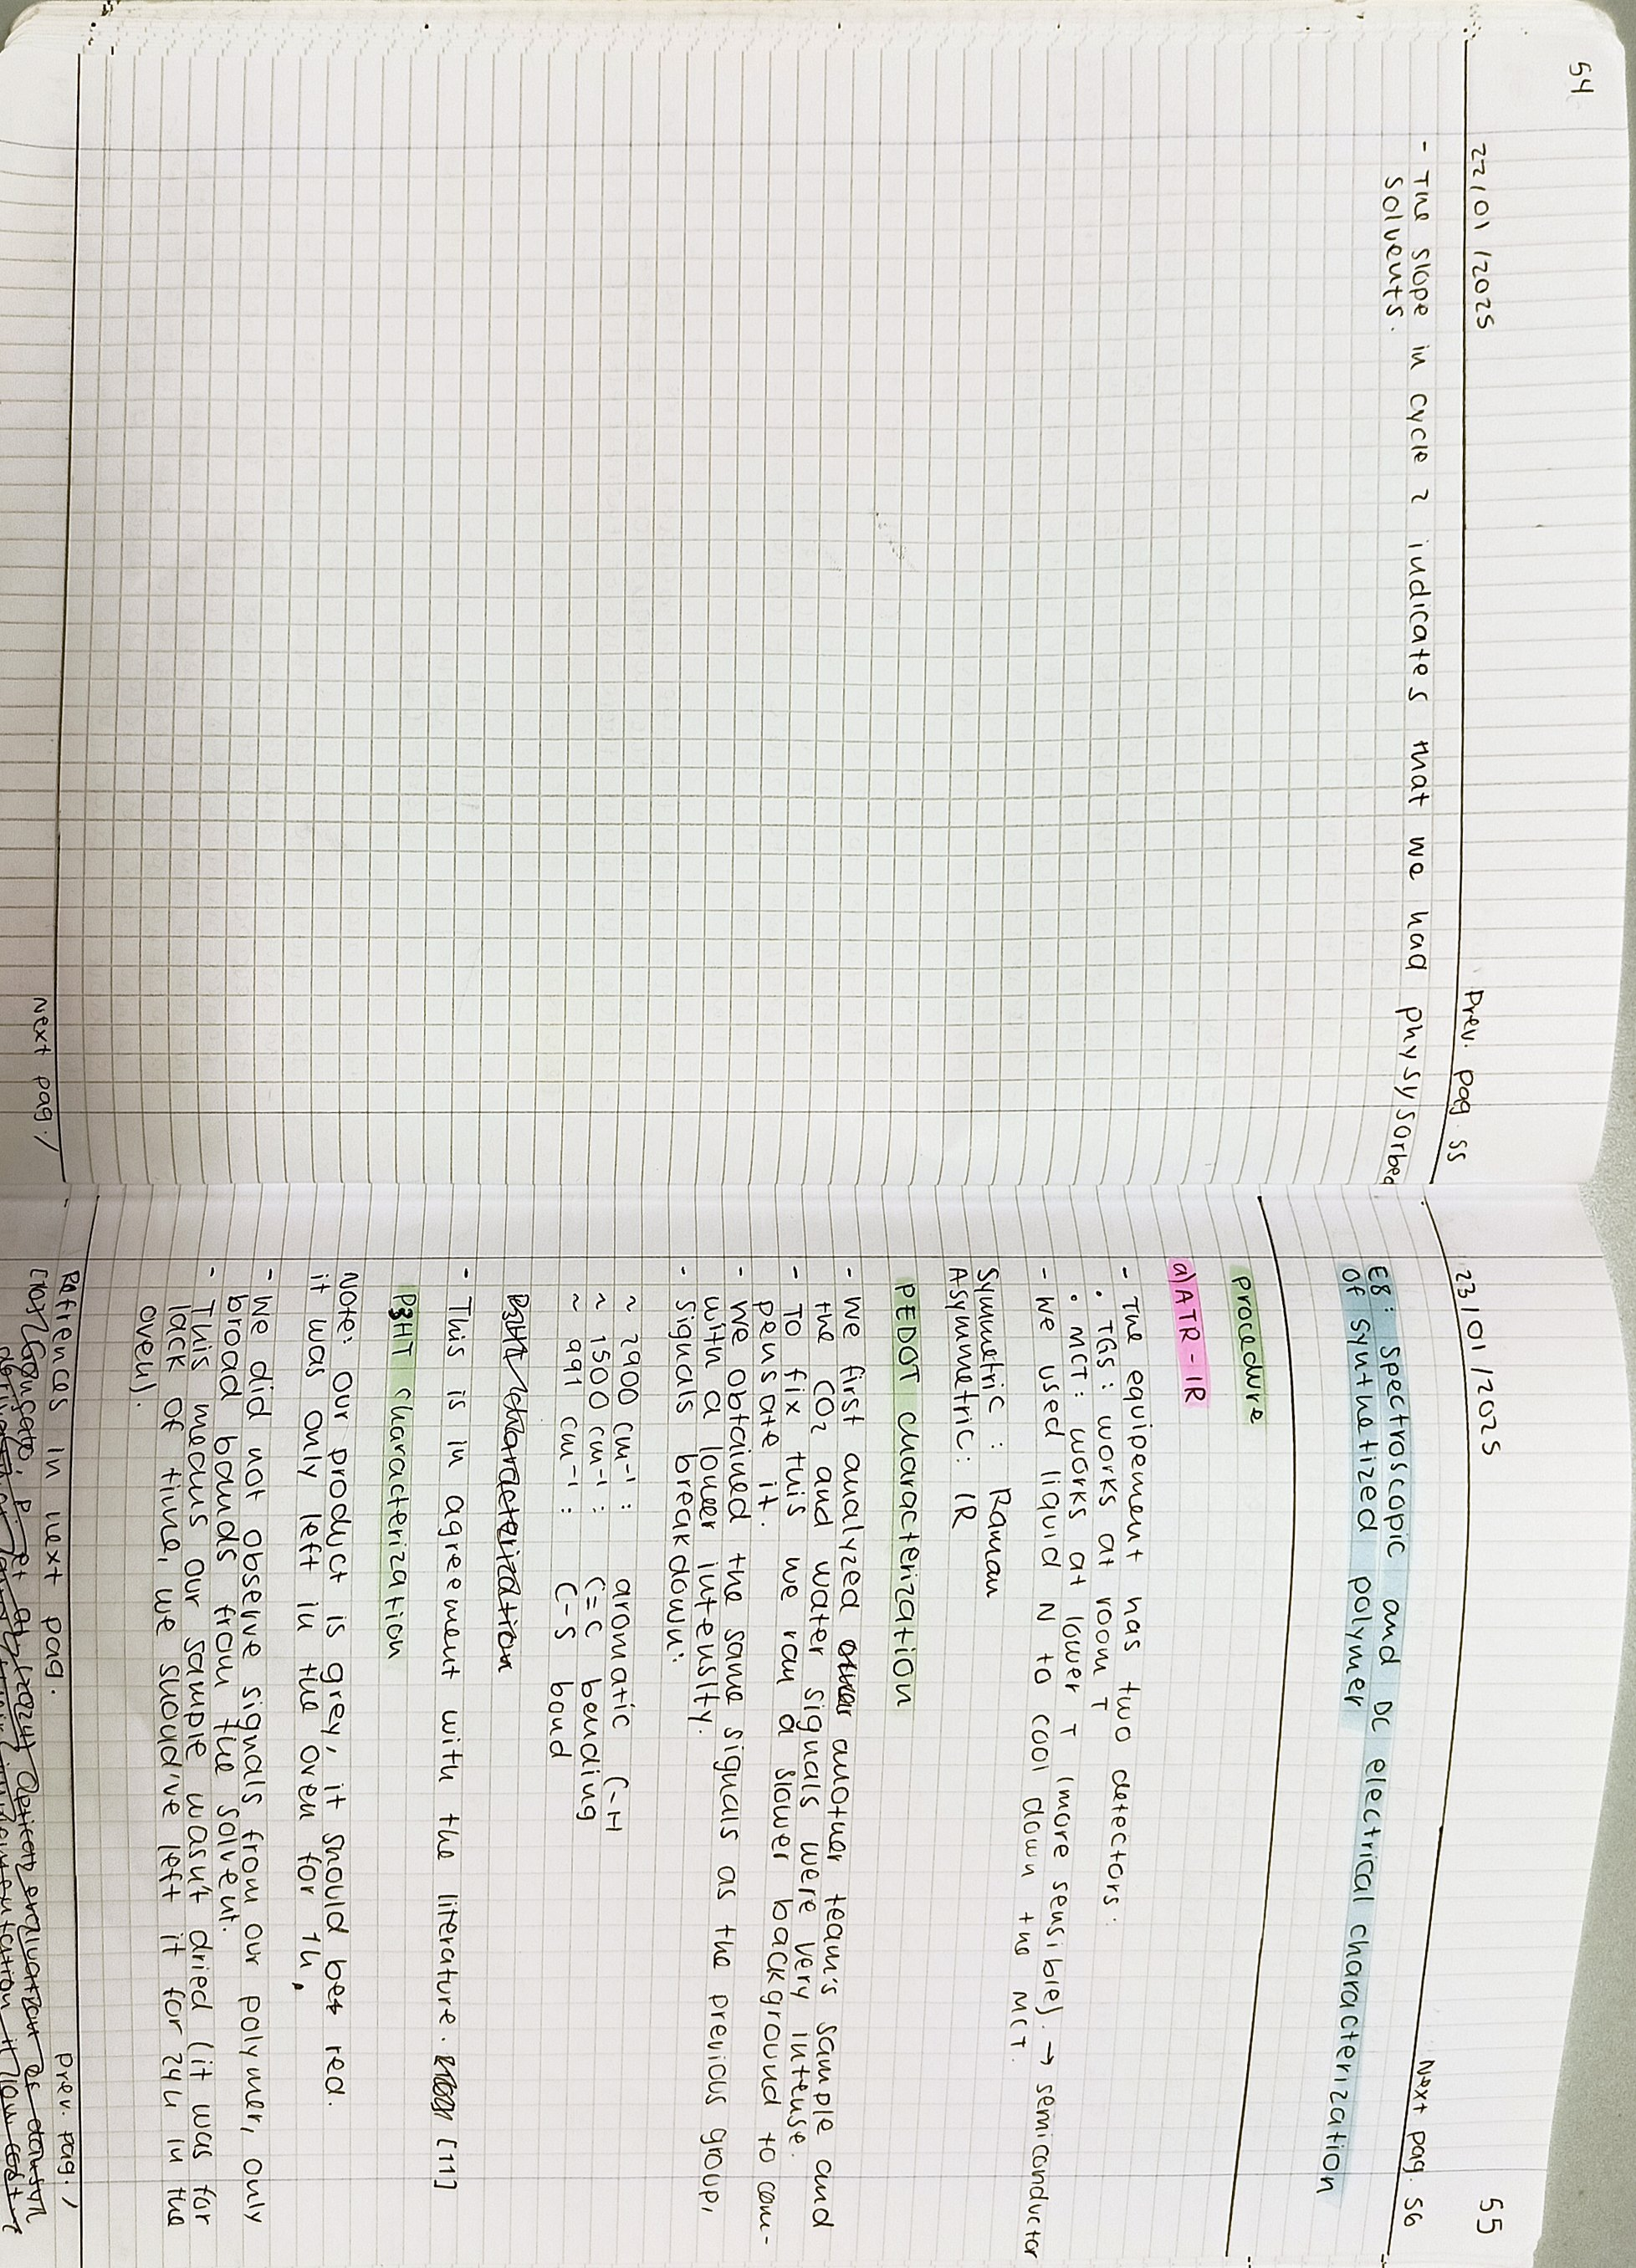
\includegraphics[width=0.6\linewidth, angle=90]{../images/compressed/IMG20250123173155.jpg}
\end{figure}


\subsection{Conductive polymer}
\begin{figure}[H]
	\centering
	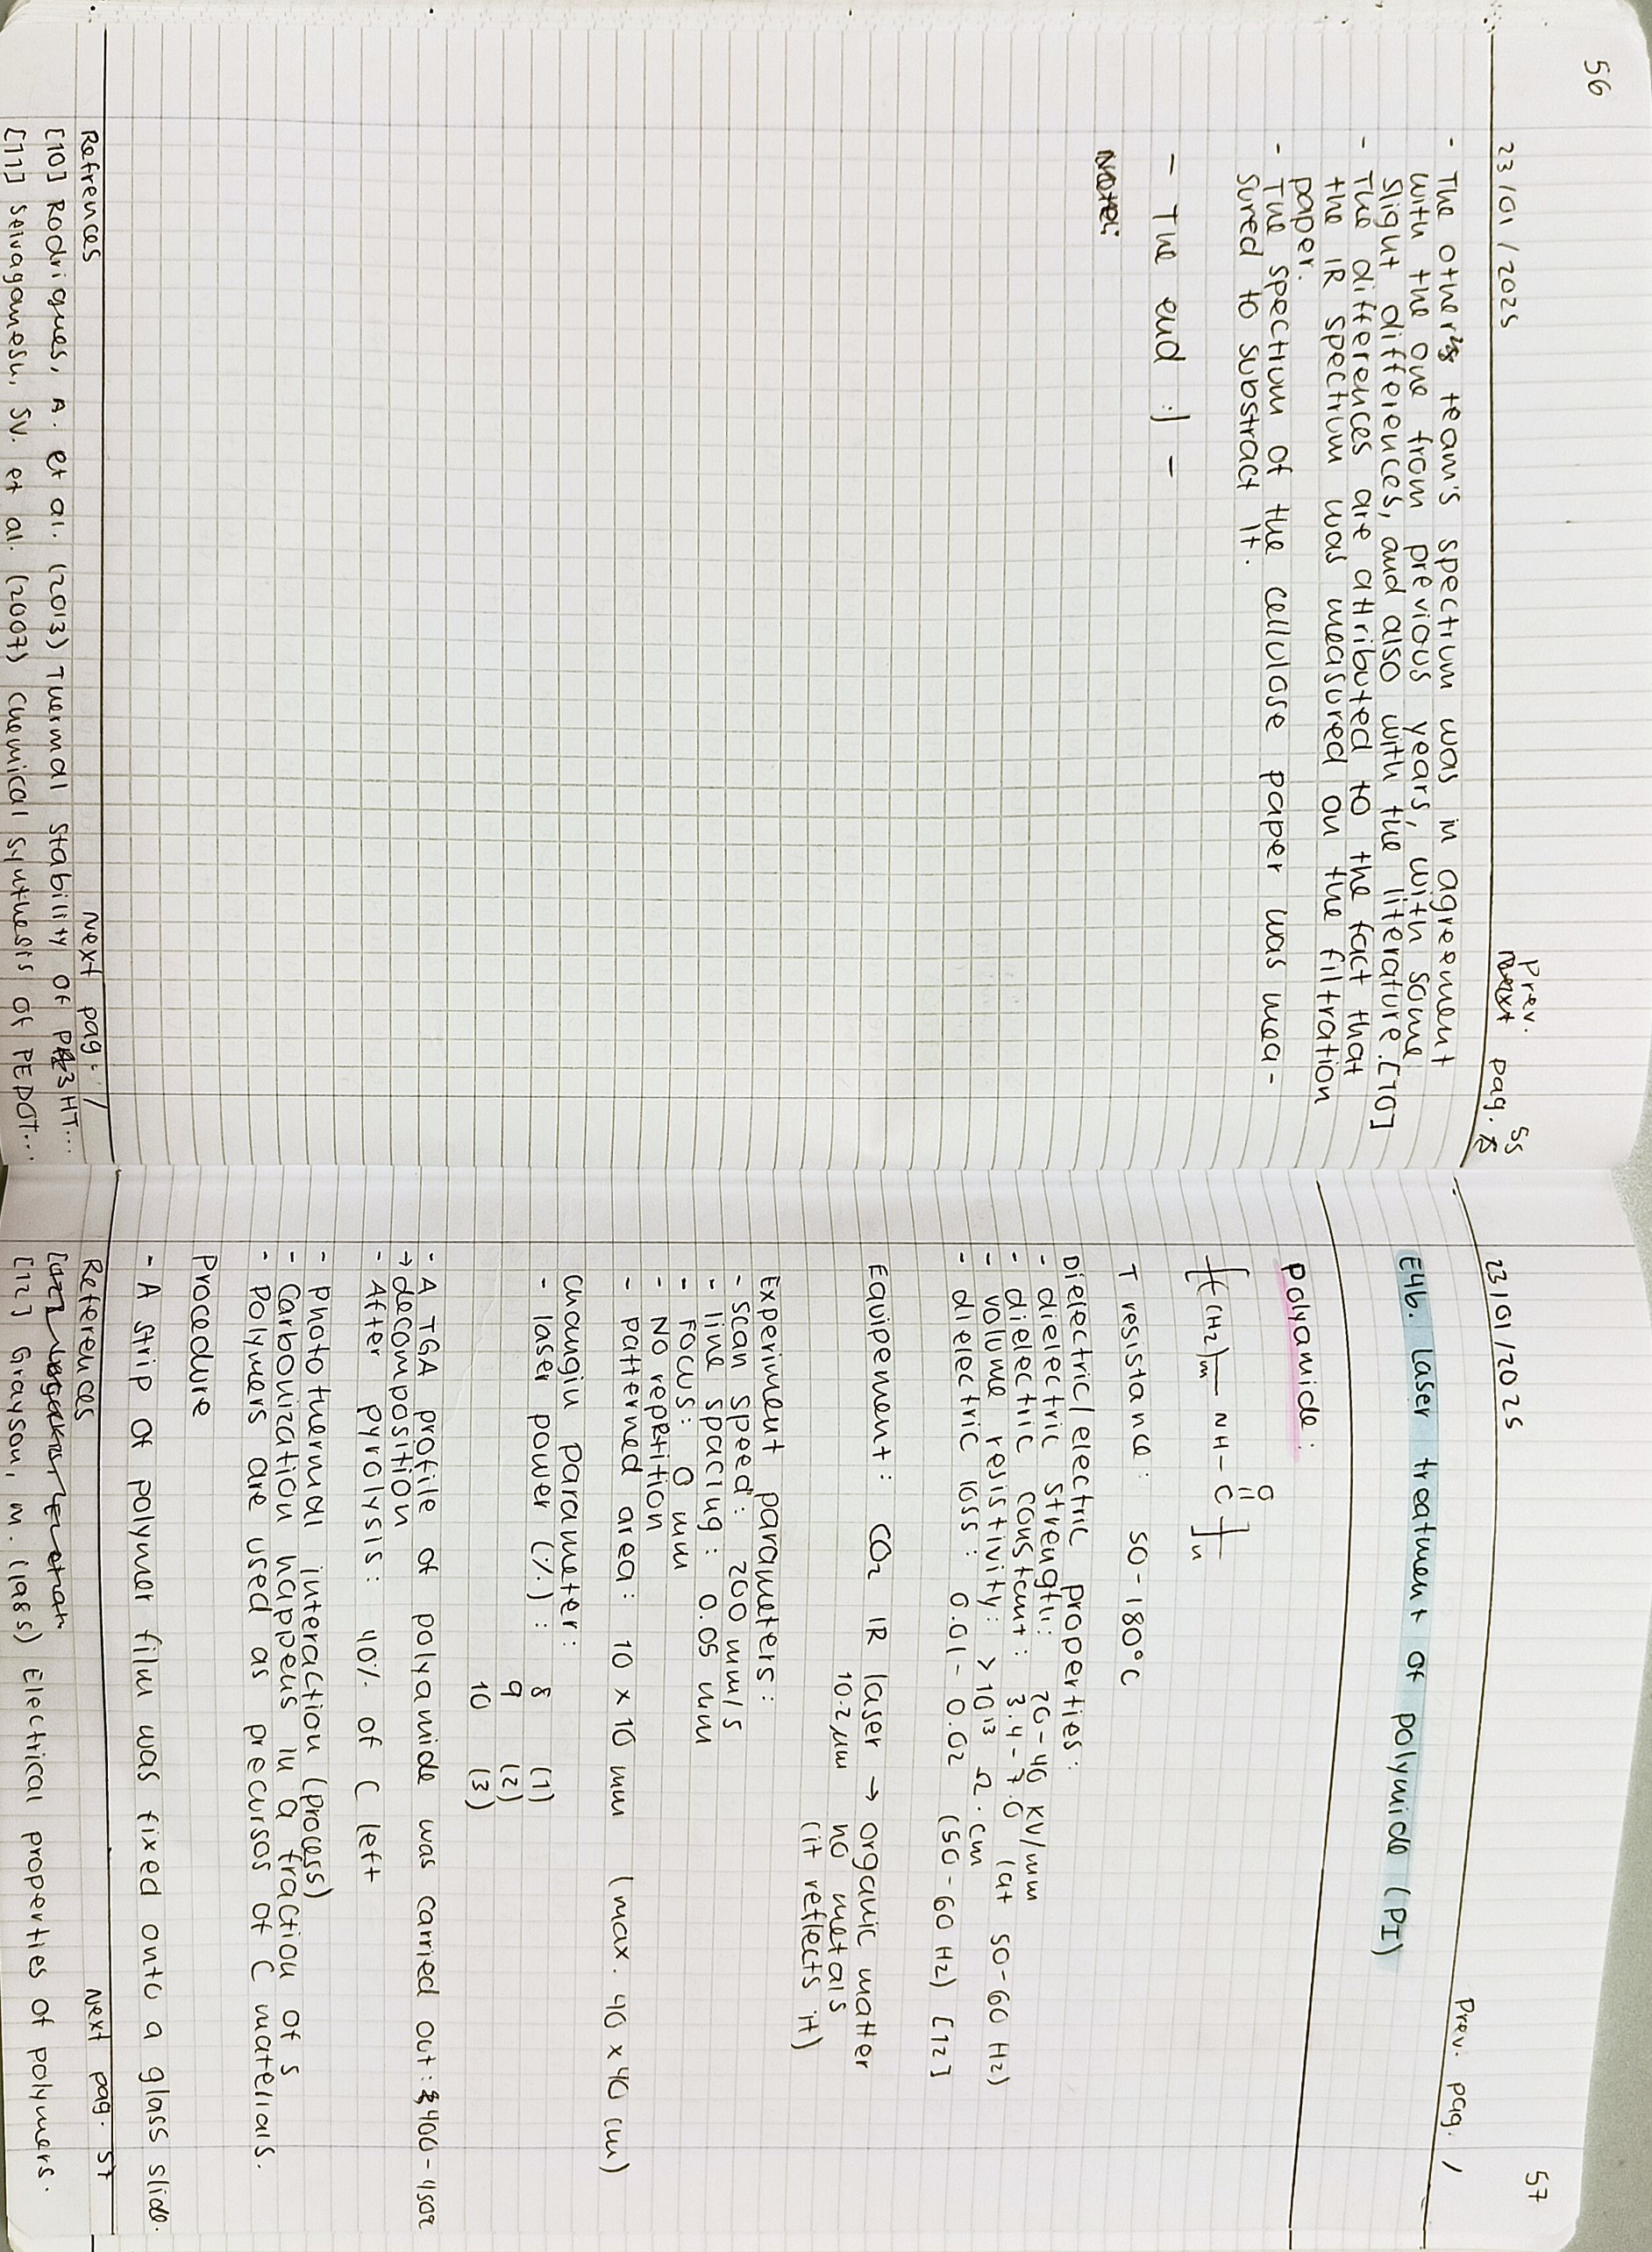
\includegraphics[width=0.6\linewidth, angle=90]{../images/compressed/IMG20250123173202.jpg}
\end{figure}
\begin{figure}[H]
	\centering
	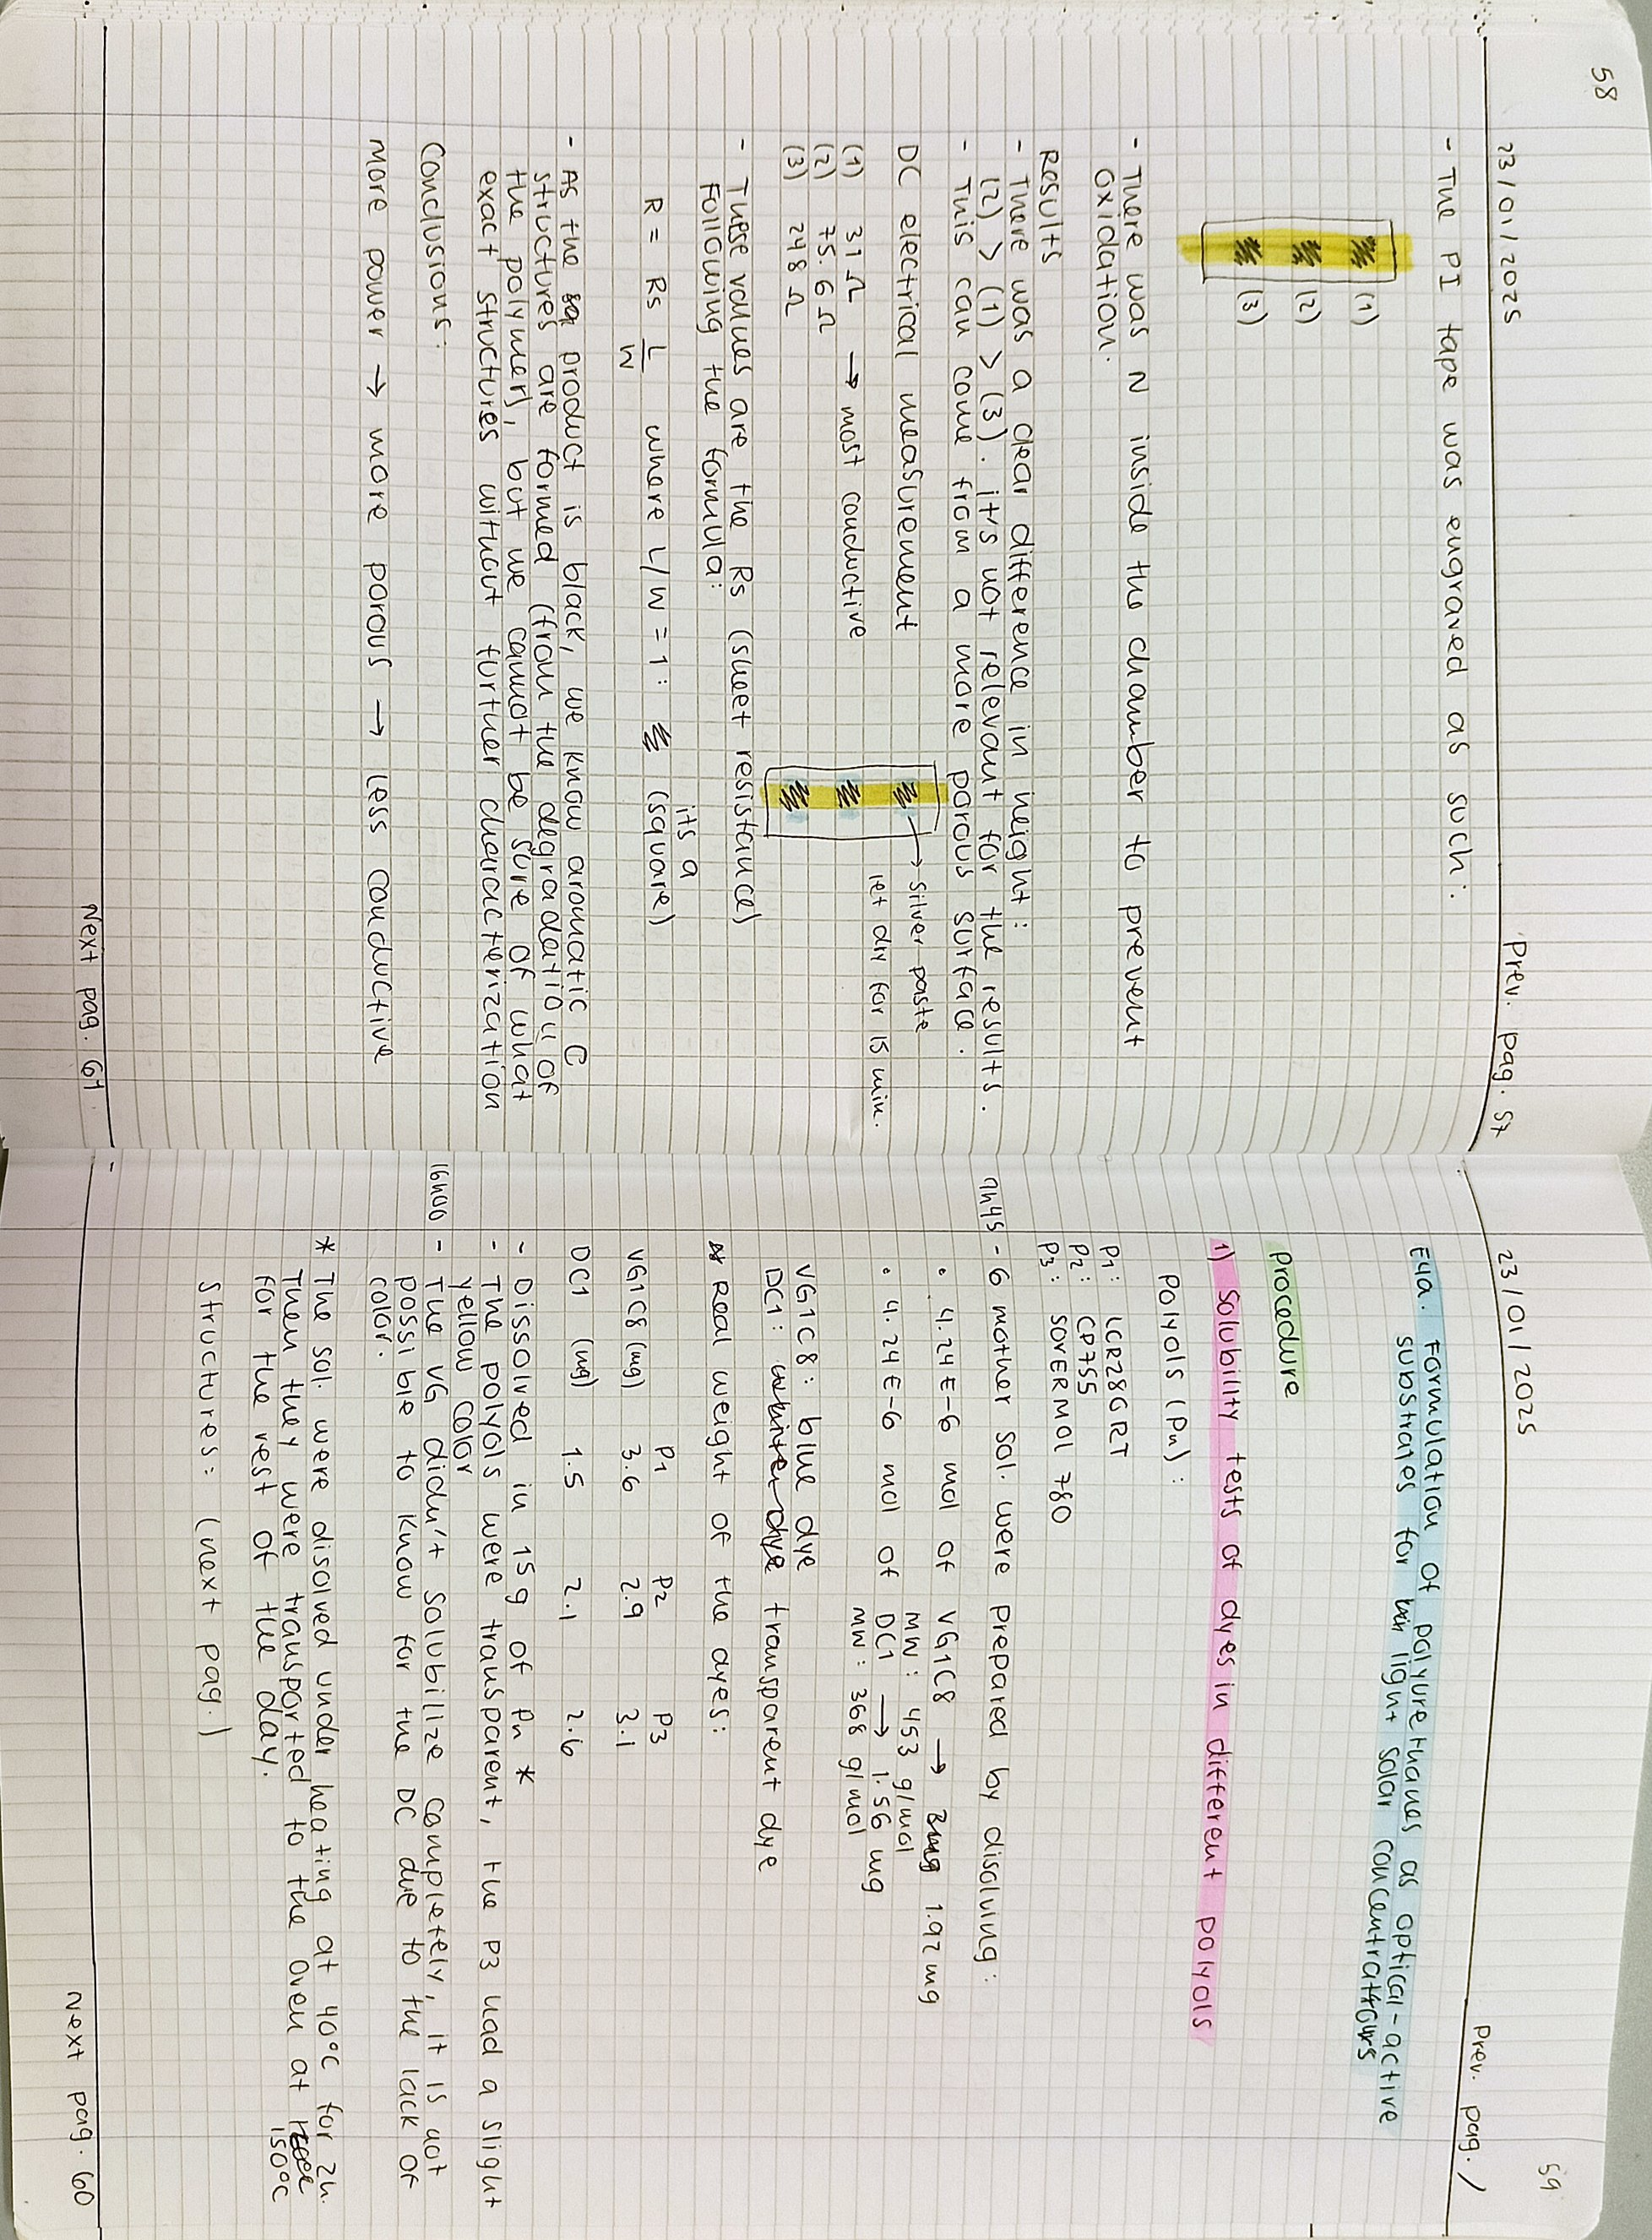
\includegraphics[width=0.6\linewidth, angle=90]{../images/compressed/IMG20250123173208.jpg}
\end{figure}
\begin{figure}[H]
	\centering
	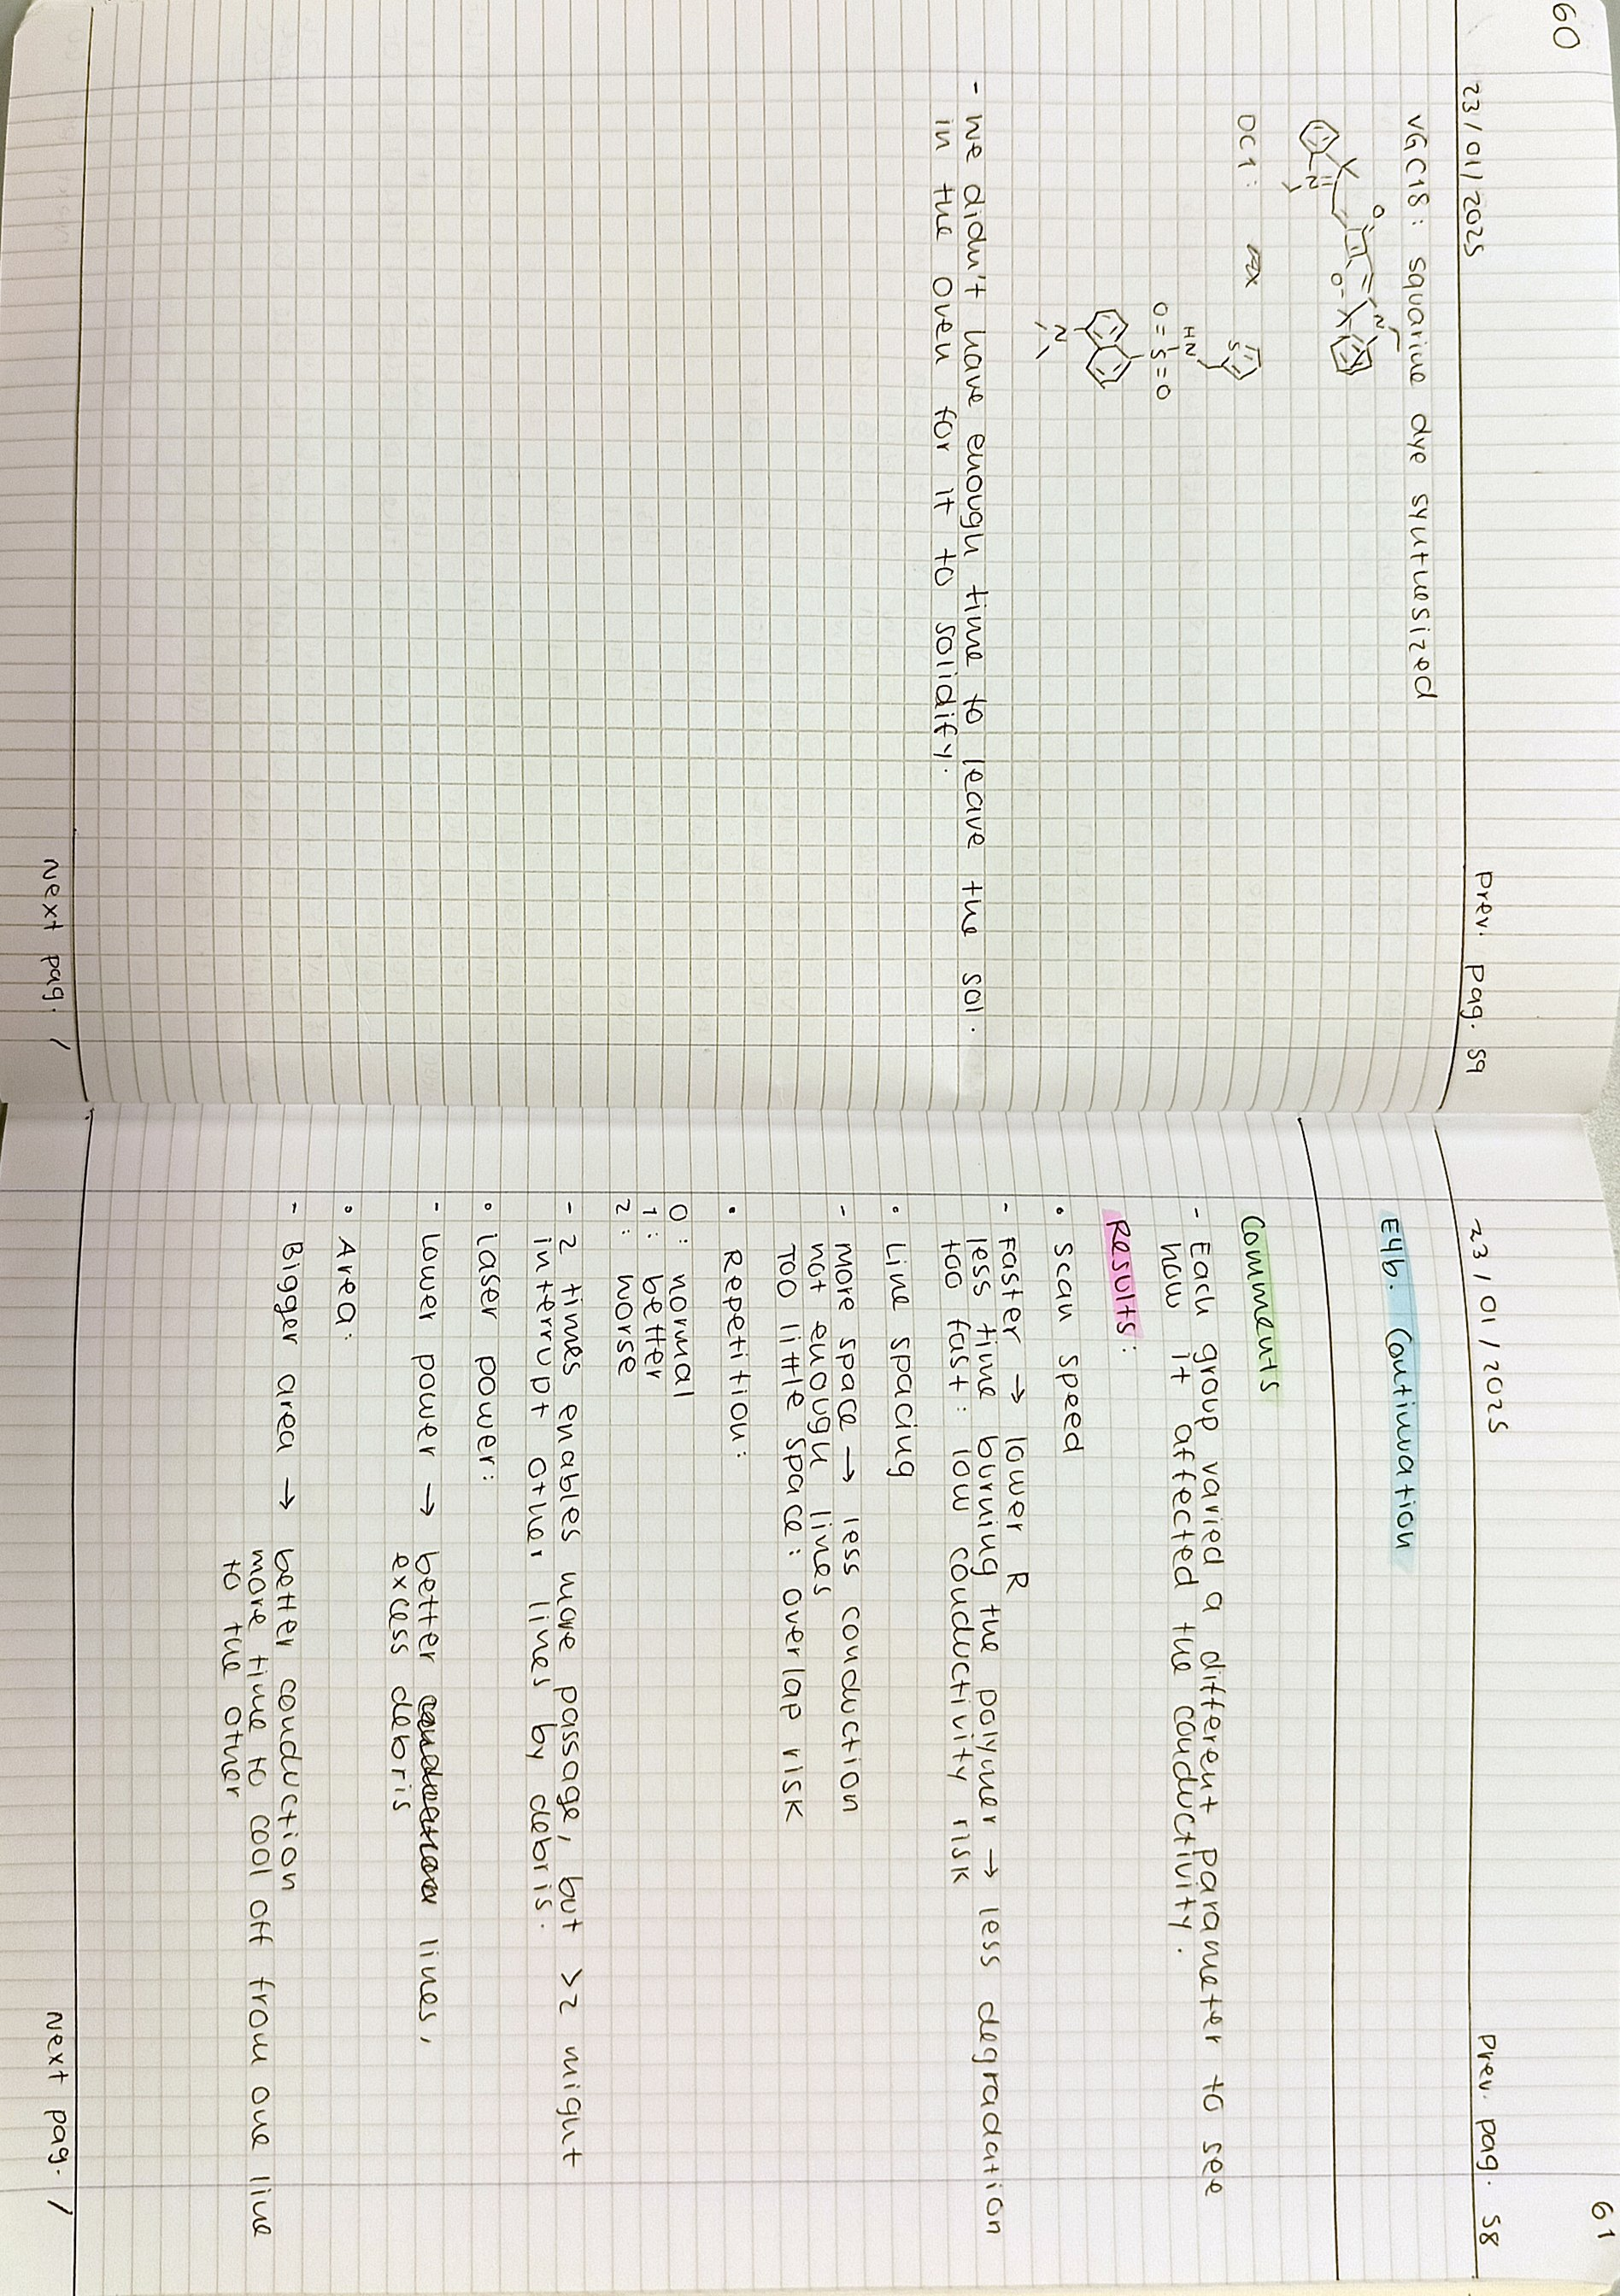
\includegraphics[width=0.6\linewidth, angle=90]{../images/compressed/IMG20250123173229.jpg}
\end{figure}


\end{document}